%%%%%%%%%%%%%%%%%%%%%%%%%%%%%%%%%%%%%%%%%%%%%%%%%%%%%%%%%%%%%%%%%%%%%%%%
%% Customizações do abnTeX2 (http://abnTeX2.googlecode.com)           %%
%% para a Universidade Estadual do Ceara - UECE                       %%
%%                                                                    %%
%% This work may be distributed and/or modified under the             %% 
%% conditions of the LaTeX Project Public License, either version 1.3 %%
%% of this license or (at your option) any later version.             %%
%% The latest version of this license is in                           %%
%%   http://www.latex-project.org/lppl.txt                            %%
%% and version 1.3 or later is part of all distributions of LaTeX     %%
%% version 2005/12/01 or later.                                       %%
%%                                                                    %%
%% This work has the LPPL maintenance status `maintained'.            %%
%%                                                                    %%
%% The Current Maintainer of this work is Thiago Nascimento           %%
%%                                                                    %%
%% Project available on: https://github.com/thiagodnf/uecetex2        %%
%%                                                                    %%
%% Further information about abnTeX2                                  %%
%% are available on http://abntex2.googlecode.com/                    %%
%%                                                                    %%
%%%%%%%%%%%%%%%%%%%%%%%%%%%%%%%%%%%%%%%%%%%%%%%%%%%%%%%%%%%%%%%%%%%%%%%%

% Preâmbulo do documento

%%%%%%%%%%%%%%%%%%%%%%%%%%%%%%%%%%%%%%%%%%%%%%%%%%%%%%%%%%%%%%%%%%%%%%%%
%% Customizações do abnTeX2 (http://abnTeX2.googlecode.com)           %%
%% para a Universidade Estadual do Ceara - UECE                       %%
%%                                                                    %%
%% This work may be distributed and/or modified under the             %% 
%% conditions of the LaTeX Project Public License, either version 1.3 %%
%% of this license or (at your option) any later version.             %%
%% The latest version of this license is in                           %%
%%   http://www.latex-project.org/lppl.txt                            %%
%% and version 1.3 or later is part of all distributions of LaTeX     %%
%% version 2005/12/01 or later.                                       %%
%%                                                                    %%
%% This work has the LPPL maintenance status `maintained'.            %%
%%                                                                    %%
%% The Current Maintainer of this work is Thiago Nascimento           %%
%%                                                                    %%
%% Project available on: https://github.com/thiagodnf/uecetex2        %%
%%                                                                    %%
%% Further information about abnTeX2                                  %%
%% are available on http://abntex2.googlecode.com/                    %%
%%                                                                    %%
%%%%%%%%%%%%%%%%%%%%%%%%%%%%%%%%%%%%%%%%%%%%%%%%%%%%%%%%%%%%%%%%%%%%%%%%

\documentclass[        
    a4paper,          % Tamanho da folha A4
    12pt,             % Tamanho da fonte 12pt
    chapter=TITLE,    % Todos os capitulos devem ter caixa alta
    section=TITLE,    % Todas as secoes devem ter caixa alta
    oneside,          % Usada para impressao em apenas uma face do papel
    english,          % Hifenizacoes em ingles
    spanish,          % Hifenizacoes em espanhol
    brazil            % Ultimo idioma eh o idioma padrao do documento
]{abntex2}

% Importações de pacotes
\usepackage[utf8]{inputenc}                         % Acentuação direta
\usepackage[T1]{fontenc}                            % Codificação da fonte em 8 bits
\usepackage{graphicx}                               % Inserir figuras
\usepackage{amsfonts, amssymb, amsmath}             % Fonte e símbolos matemáticos
\usepackage{booktabs}                               % Comandos para tabelas
\usepackage{verbatim}                               % Texto é interpretado como escrito no documento
\usepackage{multirow, array}                        % Múltiplas linhas e colunas em tabelas
\usepackage{indentfirst}                            % Endenta o primeiro parágrafo de cada seção.
\usepackage{listings}                               % Utilizar codigo fonte no documento
\usepackage{xcolor}
\usepackage{microtype}                              % Para melhorias de justificação?
\usepackage[portuguese,ruled,lined]{algorithm2e}    % Escrever algoritmos
\usepackage{algorithmic}                            % Criar Algoritmos  
\usepackage{float}									% Utilizado para criação de floats
\usepackage{newfloat}                                
\usepackage{amsgen}
\usepackage{lipsum}                                 % Usar a simulação de texto Lorem Ipsum
%\usepackage{titlesec}                              % Permite alterar os títulos do documento
\usepackage{tocloft}                                % Permite alterar a formatação do Sumário
\usepackage{etoolbox}                               % Usado para alterar a fonte da Section no Sumário
\usepackage[nogroupskip,nonumberlist,acronym]{glossaries}                % Permite fazer o glossario
\usepackage{caption,setspace}                                % Altera o comportamento da tag caption
\usepackage[alf, abnt-emphasize=bf, bibjustif, recuo=0cm, abnt-etal-cite=3, abnt-etal-list=0,abnt-etal-text=it]{abntex2cite}  % Citações padrão ABNT
%\usepackage[bottom]{footmisc}                      % Mantém as notas de rodapé sempre na mesma posição
%\usepackage{times}                                 % Usa a fonte Times
\usepackage{mathptmx}                               % Usa a fonte Times New Roman										
%\usepackage{lmodern}                               % Usa a fonte Latin Modern
%\usepackage{subfig}                                % Posicionamento de figuras
%\usepackage{scalefnt}                              % Permite redimensionar tamanho da fonte
%\usepackage{color, colortbl}                       % Comandos de cores
%\usepackage{lscape}                                % Permite páginas em modo "paisagem"
%\usepackage{ae, aecompl}                           % Fontes de alta qualidade
%\usepackage{picinpar}                              % Dispor imagens em parágrafos
%\usepackage{latexsym}                              % Símbolos matemáticos
%\usepackage{upgreek}                               % Fonte letras gregas
\usepackage{appendix}                               % Gerar o apendice no final do documento
\usepackage{paracol}                                % Criar paragrafos sem identacao
\usepackage{pdfpages}                               % Incluir pdf no documento
\usepackage{amsmath}                                % Usar equacoes matematicas
\usepackage{hyperref}								% formatação de hiperlinks
\usepackage{setspace}								% Configuração de espaçamentos
%================================================================================================================
\usepackage{lib/uecetex2}		                    % Biblioteca com as normas da UECE para trabalhos academicos
%================================================================================================================

% Organiza e gera a lista de abreviaturas, simbolos e glossario
\makeglossaries

% Gera o Indice do documento
\makeindex


%%%%%%%%%%%%%%%%%%%%%%%%%%%%%%%%%%%%%%%%%%%%%%%%%%%%%%%%%%
%%    Configuracoes do ueceTeX2 abaptado para o IFCE    %%
%%%%%%%%%%%%%%%%%%%%%%%%%%%%%%%%%%%%%%%%%%%%%%%%%%%%%%%%%%

% Opcoes disponiveis

\trabalhoacademico{tccgraduacao}
%\trabalhoacademico{tccespecializacao}
%\trabalhoacademico{dissertacao}
%\trabalhoacademico{tese}

% Define se o trabalho eh uma qualificacao
% Coloque 'nao' para versao final do trabalho

\ehqualificacao{nao}

% Remove as bordas vermelhas e verdes do PDF gerado
% Coloque 'sim' pare remover

\removerbordasdohyperlink{sim} 

% Adiciona a cor Azul a todos os hyperlinks

\cordohyperlink{nao}

%%%%%%%%%%%%%%%%%%%%%%%%%%%%%%%%%%%%%%%%%%%%%%%%%%%%%
%%          Informação sobre a IES                 %%
%%%%%%%%%%%%%%%%%%%%%%%%%%%%%%%%%%%%%%%%%%%%%%%%%%%%%

\ies{Instituto Federal de Educação, Ciência e Tecnologia do Ceará}
\iessigla{IFCE}
\campus{Tauá}
\centro{}
%%%%%%%%%%%%%%%%%%%%%%%%%%%%%%%%%%%%%%%%%%%%%%%%%%%%%
%%        Informação para TCC de Graduacao         %%
%%%%%%%%%%%%%%%%%%%%%%%%%%%%%%%%%%%%%%%%%%%%%%%%%%%%%

\graduacaoem{Tecnologia em Telemática}
\habilitacao{bacharel} % Pode colocar tambem 'licenciada'

%%%%%%%%%%%%%%%%%%%%%%%%%%%%%%%%%%%%%%%%%%%%%%%%%%%%%
%%     Informação para TCC de Especializacao       %%
%%%%%%%%%%%%%%%%%%%%%%%%%%%%%%%%%%%%%%%%%%%%%%%%%%%%%

\especializacaoem{Alfabetização de Crianças}

%%%%%%%%%%%%%%%%%%%%%%%%%%%%%%%%%%%%%%%%%%%%%%%%%%%%%
%%         Informação para Dissertacao             %%
%%%%%%%%%%%%%%%%%%%%%%%%%%%%%%%%%%%%%%%%%%%%%%%%%%%%%

\programamestrado{Programa de Pós-Graduação em Ciência da Computação}
\nomedomestrado{Mestrado Acadêmico em Ciência da Computação}
\mestreem{Ciência da Computação}
\areadeconcentracaomestrado{Ciência da Computação}

%%%%%%%%%%%%%%%%%%%%%%%%%%%%%%%%%%%%%%%%%%%%%%%%%%%%%
%%               Informação para Tese              %%
%%%%%%%%%%%%%%%%%%%%%%%%%%%%%%%%%%%%%%%%%%%%%%%%%%%%%

\programadoutorado{Programa de Pós-Graduação em Saúde Coletiva}
\nomedodoutorado{Doutorado em Saúde Coletiva}
\doutorem{Saúde Coletiva}
\areadeconcentracaodoutorado{Saúde Coletiva}

%%%%%%%%%%%%%%%%%%%%%%%%%%%%%%%%%%%%%%%%%%%%%%
%%  Informação relacionadas ao trabalho     %%
%%%%%%%%%%%%%%%%%%%%%%%%%%%%%%%%%%%%%%%%%%%%%%

\autor{Leonardo Feitosa Nogueira}
\titulo{Aplicação da Metodologia Site Survey para Análise de Cobertura e Recepção do Sinal Wi-Fi: Um Estudo de Caso no Bloco Didático do Instituto Federal do Ceará campus Tauá}
\data{2019}
\local{Tauá -- Ceará}

% Exemplo: \dataaprovacao{01 de Janeiro de 2012}
\dataaprovacao{}

%%%%%%%%%%%%%%%%%%%%%%%%%%%%%%%%%%%%%%%%%%%%%%%
%%     Informação sobre o Orientador(a)      %%
%%%%%%%%%%%%%%%%%%%%%%%%%%%%%%%%%%%%%%%%%%%%%%%

\orientador{Prof. Dr. Francisco Rafael Vasconcelos Guimarães}
\orientadories{Instituto Federal de Educação, Ciência e Tecnologia do Ceará -- IFCE}
\orientadorcentro{}
\orientadorfeminino{nao} % Coloque 'sim' se for do sexo feminino

%%%%%%%%%%%%%%%%%%%%%%%%%%%%%%%%%%%%%%%%%%%%%%%
%%      Informação sobre o Coorientador(a)   %%
%%%%%%%%%%%%%%%%%%%%%%%%%%%%%%%%%%%%%%%%%%%%%%%

% Deixe o nome do coorientador em branco para remover do documento

\coorientador{Prof. Esp. Kilbert Amorim Maciel}
\coorientadories{Instituto Federal de Educação, Ciência e Tecnologia do Ceará -- IFCE}
\coorientadorcentro{}
\coorientadorfeminino{nao} % Coloque 'sim' se for do sexo feminino

%%%%%%%%%%%%%%%%%%%%%%%%%%%%%%%%%%%%%%%%%%%%%%%
%%      Informação sobre a banca             %%
%%%%%%%%%%%%%%%%%%%%%%%%%%%%%%%%%%%%%%%%%%%%%%%

% Atenção! Deixe o nome do membro da banca em branco para remover da folha de aprovacao

% Exemplo de uso:
% \membrodabancadois{Prof. Dr. Fulano de Tal}
% \membrodabancadoisies{Universidade Estadual do Ceará - UECE}

\membrodabancadois{Prof. Dr. Daniel Costa Araújo}
\membrodabancadoiscentro{}
\membrodabancadoisies{Centro Universitário 7 de Setembro -- UNI7}

\membrodabancatres{Prof. Me. Francisco Hugo Costa Neto}
\membrodabancatrescentro{}
\membrodabancatresies{Centro Universitário Faculdade Nordeste -- UniFanor}

\membrodabancaquatro{Prof. Esp. Francisco Luciano Castro Martins Júnior}
\membrodabancaquatrocentro{}
\membrodabancaquatroies{Instituto Federal de Educação, Ciência e Tecnologia do Ceará -- IFCE}

\begin{document}	

	% Se o seu trabalho é em ingles, descomente a linha a seguir
	%\selectlanguage{english}

	% Elementos pré-textuais
	\imprimircapa
	\imprimirfolhaderosto{}
%	\imprimirfichacatalografica{elementos-pre-textuais/ficha-catalografica}
%	\imprimirerrata{elementos-pre-textuais/errata}
	\imprimirfolhadeaprovacao{elementos-pre-textuais/folha-de-aprovacao-assinada}
	\imprimirdedicatoria{elementos-pre-textuais/dedicatoria}
	\imprimiragradecimentos{elementos-pre-textuais/agradecimentos}
	\imprimirepigrafe{elementos-pre-textuais/epigrafe}
	\imprimirresumo{elementos-pre-textuais/resumo}
	\imprimirabstract{elementos-pre-textuais/abstract}
	\imprimirlistadeilustracoes
	\imprimirlistadetabelas
	%\imprimirlistadequadros
	%\imprimirlistadealgoritmos
	%\imprimirlistadecodigosfonte
	\imprimirlistadeabreviaturasesiglas{elementos-pre-textuais/lista-de-abreviaturas-e-siglas}
	%\imprimirlistadesimbolos{elementos-pre-textuais/lista-de-simbolos}   
	\imprimirsumario
	
	% Elementos textuais
	\textual
	% Arquivos de Exemplo
%	\chapter{Introdução}
\label{cap:introducao}

Em 1971, o sistema Aloha\footnote{Originalmente, o sistema Aloha, desenvolvido por Norman Abramson em 1970, na Universidade do Havaí, funcionava como um protocolo para sistemas de comunicação via radiofrequência para o acesso remoto entre computadores enviando pacotes num sistema de radiocomunicação \cite{abramson1970acm, haykin2009}.} estabeleceu e operou uma rede de dados terrestres (AlohaNet) no estado americano do Havaí. Em 1973, ao sofrer uma adaptação, o sistema Aloha usou um transponder acoplada em um satélite experimental da Agência Espacial Americana (NASA, do inglês, \textit{National Aeronautics and Space Administration}) (ATS-1) para demonstrar uma rede internacional de dados via satélite conectando a NASA, na Califórnia, e cinco universidades nos Estados Unidos, Japão e Austrália, fornecendo a primeira demonstração pública de uma rede de dados por pacotes sem fio \cite{abramson1970acm, SchwartzAbramson2009ieee}. Também em 1973, o rede AlohaNet foi vinculada à ARPANet\footnote{A primeira rede de computadores por comutação de pacotes e uma ancestral direta da Internet pública de hoje \cite{kurose2013}.} (do inglês, \textit{Advanced Research Projects Agency Network}) \cite{abramson1970acm, SchwartzAbramson2009ieee}.

Mesmo com limitações como largura de banda e tecnologia de transmissão, foi graças ao pioneirismo do sistema Aloha, que as redes de comutação sem fio, conhecidas como \textit{wireless} ou ainda WLANs (do inglês, \textit{Wireless Local Area Network}) surgiram como redes complementares às redes cabeadas tradicionais. Essa tecnologia de comunicação se desenvolveu devido a necessidade de implementação de um método alternativo de conexão que não privasse a movimentação do usuário a uma posição fixa durante uma transmissão/recepção de dados na rede. O tempo passou e a tecnologia evoluiu, deixou de ser restrito ao meio acadêmico e militar e se tornou acessível a empresas e ao usuário doméstico. Nos dias de hoje podemos pensar em redes \textit{wireless} como uma alternativa bastante interessante em relação às redes cabeadas. Suas aplicações são muitas e variadas e o fato de ter a mobilidade como principal característica, tem facilitado a sua aceitação, principalmente nas empresas (FARIAS, 2005).

Com o advento de \textit{notebooks}, \textit{tablets}, \textit{smartphones} e a promessa de acesso desimpedido à Internet global de qualquer lugar por meio das comunicações sem fio, a qualquer hora, assistimos a uma explosão semelhante da utilização de dispositivos sem fio para acesso à Internet em comparação ao dos telefones móveis, não só através da rede de telefonia móvel, agora plenamente possível, mas também por meio das redes Wi-Fi. O uso deste tipo de rede está se tornando cada vez mais comum, não só nos ambientes domésticos e corporativos, mas também em locais públicos (bares, lanchonetes, shoppings, aeroportos, etc) e em instituições acadêmicas. Independentemente do crescimento futuro de equipamentos sem fio para Internet, já ficou claro que as redes sem fio e os serviços móveis relacionados que elas possibilitam vieram para ficar (KUROSE; ROSS, 2013; GAST, 2002).

No período em que as redes locais cabeadas (LAN -- \textit{Local Area Network}, do inglês)  dominavam a infraestrutura de rede de computadores, somente era possível conectar computadores à Internet e entre si por meio de cabos padrão Ethernet. Este tipo de conexão é bastante popular, mas conta com algumas limitações, por exemplo: só se pode movimentar o computador até o limite de alcance do cabo; ambientes com um grande número computadores podem exigir adaptações na estrutura do prédio para a passagem dos fios; em uma residência, pode ser necessário realizar perfurações na parede para que os cabos alcancem outros cômodos; a manipulação constante ou incorreta pode fazer com que o conector do cabo de rede se danifique. Com exceção da mobilidade, o restante das alegações implica em investimento financeiro direto por parte das empresas e também para o usuário doméstico. Felizmente, as redes sem fio Wi-Fi surgiram para eliminar estas limitações. Como consequência, alcançaram rapidamente uma disseminação generalizada tanto no espaço comercial quanto no residencial (ALECRIM, 2008).

%\lipsum[5]
%\lipsum[6]
%\lipsum[7]

\newpage
\section{Motivação}
\label{sec:motivacao}

%\lipsum[3]
%\lipsum[4]

\section{Objetivos}
\label{sec:objetivos}

Interdum et malesuada fames ac ante ipsum primis in faucibus. Lorem ipsum dolor sit amet, consectetur adipiscing elit. Ut ex tellus, sodales in euismod at, ultricies quis leo \cite{alecrim2008site}.

\subsection{Objetivo Geral}
\label{sec:objetivo-geral}

Integer imperdiet ac magna eu pulvinar. Aliquam erat volutpat. Etiam molestie, nulla a egestas aliquet, velit augue congue metus, et ultricies metus massa vel nibh. Vivamus viverra commodo finibus. Nam elementum convallis accumsan. Quisque tincidunt purus nisl, tincidunt ultricies odio ultrices eu.

\subsection{Objetivos Específicos}
\label{sec:objetivos-especificos}

Lorem ipsum dolor sit amet, consectetur adipiscing elit. Duis scelerisque, velit at facilisis hendrerit, dui eros lacinia metus, non maximus mi tortor ut lectus. Donec hendrerit leo ut consectetur tincidunt. 

	\begin{alineas}
		\item Lorem ipsum dolor sit amet, consectetur adipiscing elit. Nunc dictum sed tortor nec viverra.
		\item Praesent vitae nulla varius, pulvinar quam at, dapibus nisi. Aenean in commodo tellus. Mauris molestie est sed justo malesuada, quis feugiat tellus venenatis.
		\item Praesent quis erat eleifend, lacinia turpis in, tristique tellus. Nunc dictum sed tortor nec viverra.
		\item Mauris facilisis odio eu ornare tempor. Nunc dictum sed tortor nec viverra.
		\item Curabitur convallis odio at eros consequat pretium.
	\end{alineas}
%	\chapter{Fundamentação Teórica}
\label{cap:fundamentacao-teorica}

Integer non lacinia magna. Aenean tempor lorem tellus, non sodales nisl commodo ut. Proin mattis placerat risus sit amet laoreet. Praesent sapien arcu, maximus ac fringilla efficitur, vulputate faucibus sem. Donec aliquet velit eros, sit amet elementum dolor pharetra eget. Integer eget mattis libero

\section{Fundamentação Teórica A}
\label{sec:fundamentacao-teorica-a}

\lipsum[10]

	\begin{figure}[h!]
		\centering
		\Caption{\label{fig:exemplo-1} Lorem ipsum dolor sit amet, consectetur adipiscing elit. Suspendisse commodo lectus et augue elementum varius.}	
		\UECEfig{}{
			\fbox{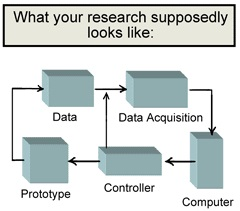
\includegraphics[width=8cm]{figuras/figura-1}}
		}{
			\Fonte{Elaborado pelo autor}
		}	
	\end{figure}
	
\lipsum[11]


\section{Fundamentação Teórica B}
\label{sec:fundamentacao-teorica-b}

Integer non lacinia magna. Aenean tempor lorem tellus, non sodales nisl commodo ut. Proin mattis placerat risus sit amet laoreet. Praesent sapien arcu, maximus ac fringilla efficitur, vulputate faucibus sem. Donec aliquet velit eros, sit amet elementum dolor pharetra eget. Integer eget mattis libero. Praesent ex velit, pulvinar at massa vel, fermentum dictum mauris. Ut feugiat accumsan augue, et ultrices ipsum euismod vitae

	\begin{figure}[h!]
		\centering
		\Caption{\label{fig:exemplo-2} Maecenas luctus augue odio, sed tincidunt nunc posuere nec}	
		\UECEfig{}{
			\fbox{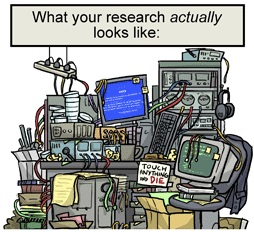
\includegraphics[width=8cm]{figuras/figura-2}}
		}{
			\Fonte{Elaborado pelo autor}			
		}	
	\end{figure}

Nunc ac pretium dui. Mauris aliquam dapibus nulla ac mattis. Aenean non tortor volutpat, varius lectus vitae, accumsan nibh. Cras pretium vestibulum enim, id ullamcorper tortor ultrices non. Integer sodales viverra faucibus. Curabitur at dui lacinia, rhoncus lacus at, blandit metus. Integer scelerisque non enim quis ornare.

\lipsum[13]

	\begin{table}[h!]	
		\centering
		\Caption{\label{tab:exemplo-1} Duis faucibus, enim quis tincidunt pellentesque, nisl leo varius nulla, vitae tempus dui mauris ac ante purus lorem}		
		\UECEtab{}{
			\begin{tabular}{cll}
				\toprule
				Ranking & Exon Coverage & Splice Site Support \\
				\midrule \midrule
				E1 & Complete coverage by a single transcript & Both splice sites\\
				E2 & Complete coverage by more than a single transcript & Both splice sites\\
				E3 & Partial coverage & Both splice sites\\
				E4 & Partial coverage & One splice site\\
				E5 & Complete or partial coverage & No splice sites\\
				E6 & No coverage & No splice sites\\
				\bottomrule
			\end{tabular}
		}{
		\Fonte{Elaborado pelo autor}
	}
	\end{table}

Duis faucibus, enim quis tincidunt pellentesque, nisl leo varius nulla, vitae tempus dui mauris ac ante. Quisque purus lorem, pharetra sit amet lobortis eu, vehicula vitae purus. Ut varius, erat nec vehicula elementum, risus est tempus justo, nec vulputate augue leo egestas metus.

	\begin{figure}[h!]
		\centering
		\Caption{\label{fig:exemplo-3} Ut posuere, ex quis sagittis auctor, magna massa euismod felis}	
		\UECEfig{}{
			\fbox{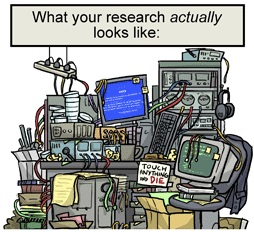
\includegraphics[width=8cm]{figuras/figura-2}}
		}{
		\Fonte{Elaborado pelo autor}			
	}	
	\end{figure}

\lipsum[14]

	\begin{table}[h!]	
		\centering
		\Caption{\label{tab:exemplo-2} Etiam molestie, nulla a egestas aliquet, velit augue congue metus}		
		\UECEtab{}{
			\begin{tabular}{ccll}
				\toprule
				Quisque & pharetra & tempus & vulputate \\
				\midrule \midrule
				E1 & Complete coverage by a single transcript & Both splice sites\\
				E2 & Complete coverage by more than a single transcript & Both splice sites\\
				E3 & Partial coverage & Both splice sites & Both \\
				E4 & Partial coverage & One splice site & Both \\
				E5 & Complete or partial coverage & No splice sites & Both\\
				E6 & No coverage & No splice sites\\
				\bottomrule
			\end{tabular}
		}{
		\Fonte{Elaborado pelo autor}
	}
	\end{table}
	
Duis faucibus, enim quis tincidunt pellentesque, nisl leo varius nulla, vitae tempus dui mauris ac ante. Quisque purus lorem, pharetra sit amet lobortis eu, vehicula vitae purus.
\acrlong{DATASUS},\acrlong{DNV},\acrlong{DO},\acrlong{ESF},\acrlong{IBGE},\acrlong{MFC},\acrlong{MI},\acrlong{MS},\acrlong{NV},\acrlong{ODM},\acrlong{OI},\acrlong{OMS},\acrlong{ONU},\acrlong{PNI},\acrlong{PSF},\acrlong{RIPSA},\acrlong{RN},\acrlong{SIM},\acrlong{SINASC},\acrlong{SUS},\acrlong{TMI},\acrlong{TMMFC}

\begin{alineascomponto}
	\item Integer non lacinia magna. Aenean tempor lorem tellus, non sodales nisl commodo ut
	\item Proin mattis placerat risus sit amet laoreet. Praesent sapien arcu, maximus ac fringilla efficitur, vulputate faucibus sem. Donec aliquet velit eros, sit amet elementum dolor pharetra eget
	\item Integer eget mattis libero. Praesent ex velit, pulvinar at massa vel, fermentum dictum mauris. Ut feugiat accumsan augue, et ultrices ipsum euismod vitae
	\begin{subalineascomponto}
		\item Integer non lacinia magna. Aenean tempor lorem tellus, non sodales nisl commodo ut
		\item Proin mattis placerat risus sit amet laoreet.
	\end{subalineascomponto}
\end{alineascomponto}
%	\chapter{Trabalhos Relacionados}
\label{cap:trabalhos-relacionados}

Integer non lacinia magna. Aenean tempor lorem tellus, non sodales nisl commodo ut. Proin mattis placerat risus sit amet laoreet. Praesent sapien arcu, maximus ac fringilla efficitur, vulputate faucibus sem. Donec aliquet velit eros, sit amet elementum dolor pharetra eget. Integer eget mattis libero

\section{Trabalho Relacionado A}
\label{sec:trabalho-relacionado-a}

\lipsum[10]

	\begin{figure}[h!]
		\centering
		\Caption{\label{fig:exemplo-1} Lorem ipsum dolor sit amet, consectetur adipiscing elit. Suspendisse commodo lectus et augue elementum varius.}	
		\UECEfig{}{
			\fbox{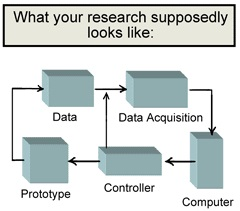
\includegraphics[width=8cm]{figuras/figura-1}}
		}{
			\Fonte{Elaborado pelo autor}
		}	
	\end{figure}
	
\lipsum[11]

\section{Trabalho Relacionado B}
\label{sec:trabalho-relacionado-b}

Integer non lacinia magna. Aenean tempor lorem tellus, non sodales nisl commodo ut. Proin mattis placerat risus sit amet laoreet. Praesent sapien arcu, maximus ac fringilla efficitur, vulputate faucibus sem. Donec aliquet velit eros, sit amet elementum dolor pharetra eget. Integer eget mattis libero. Praesent ex velit, pulvinar at massa vel, fermentum dictum mauris. Ut feugiat accumsan augue, et ultrices ipsum euismod vitae

	\begin{figure}[h!]
		\centering
		\Caption{\label{fig:exemplo-2} Maecenas luctus augue odio, sed tincidunt nunc posuere nec}	
		\UECEfig{}{
			\fbox{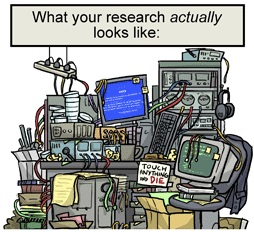
\includegraphics[width=8cm]{figuras/figura-2}}
		}{
			\Fonte{Elaborado pelo autor}			
		}	
	\end{figure}

Nunc ac pretium dui. Mauris aliquam dapibus nulla ac mattis. Aenean non tortor volutpat, varius lectus vitae, accumsan nibh. Cras pretium vestibulum enim, id ullamcorper tortor ultrices non. Integer sodales viverra faucibus. Curabitur at dui lacinia, rhoncus lacus at, blandit metus. Integer scelerisque non enim quis ornare.

	\begin{quadro}[h!]	
		\centering
		\Caption{\label{qua:exemplo-1} Praesent ex velit, pulvinar at massa vel, fermentum dictum mauris. Ut feugiat accumsan augue}		
		\UECEqua{}{
			\begin{tabular}{|c|c|l|l|}
				\hline
				Quisque & pharetra & tempus & vulputate \\
				\hline
				E1 & Complete coverage by a single transcript & Both  & Complete\\
				\hline
				E2 & Complete coverage by more than & Both splice sites & Complete\\
				\hline
				E3 & Partial coverage & Both splice sites & Both \\				
				\hline
			\end{tabular}
		}{
			\Fonte{Elaborado pelo autor}
		}
	\end{quadro}
	
\lipsum[20]

	
	\begin{quadro}[h!]	
		\centering
		\Caption{\label{qua:exemplo-2} Duis faucibus, enim quis tincidunt pellentesque}		
		\UECEqua{}{
			\begin{tabular}{|c|c|}
				\hline
				Quisque & pharetra \\
				\hline
				E1 & Complete coverage by a single transcript \\
				\hline
				E2 & Complete coverage by more than \\
				\hline
				E3 & Partial coverage \\
				\hline
				E4 & Partial coverage \\
				\hline
				E5 & Partial coverage \\
				\hline
				E6 & Partial coverage \\
				\hline
				E7 & Partial coverage \\
				\hline
			\end{tabular}
		}{
			\Fonte{Elaborado pelo autor}
		}
	\end{quadro}

\lipsum[21]

Integer non lacinia magna. Aenean tempor lorem tellus, non sodales nisl commodo ut. Proin mattis placerat risus sit amet laoreet. Praesent sapien arcu, maximus ac fringilla efficitur, vulputate faucibus sem. Donec aliquet velit eros, sit amet elementum dolor pharetra eget. Integer eget mattis libero.
\Gls{ambiguidade}
\Gls{braile}
\Gls{coerencia}
\Gls{dialetos}
\Gls{elipse}
\Gls{locucao-adjetiva}
\Gls{modificadores}
\Gls{paronimos}
\Gls{sintese}
\Gls{borboleta}
	%\chapter{Metodologia}
\label{chap:metodologia}

\lipsum[2]
\lipsum[12]

O autor \cite{lamport1986latex} e \cite{Maia2011} \lipsum[2] 

\begin{table}[h!]
	\Caption{\label{tabela-ibge} Um Exemplo de tabela alinhada que pode ser longa ou curta, conforme padrão IBGE. conforme padrão IBGE. conforme padrão IBGE. conforme padrão IBGE. conforme padrão IBGE. conforme padrão IBGE. conforme padrão IBGE. conforme padrão IBGE. conforme padrão IBGE. conforme padrão IBGE. conforme padrão IBGE.}%
	\IBGEtab{}{%
		\begin{tabular}{ccc}
			\toprule
			Material da parede & Espessura & $k=1$ \\
			\toprule %\midrule
			Madeira compensada & 0.4 cm & $L_{w1I} = 0.9\ dB$ \\
			
			Parede de gesso -- parede de gesso \\ rebocada com 1 mm de espessura máx. de gesso & 13.5 cm & $L_{w2I} = 3.0\ dB$ \\
			
			Cartão áspero & 1.5 cm & $L_{w3I} = 1.0\ dB$ \\
			
			Prato de vidro &  & $L_{w4I} = 2.5\ dB$ \\
			
			Janela de vidro duplo -- com uma camada \\ de ar de 12 mm & 2.0 cm & $L_{w5I} = 12\ dB$ \\
			
			Parede de bloco de concreto -- bloco \\ de concreto armado & 30.2 cm & $L_{w6I} = 10\ dB$ \\
			\bottomrule
		\end{tabular}%
	}{%
	\Fonte{Produzido pelos autores}%
	\Nota{Esta éuma nota, que diz que os dados são baseados na
		regressão linear.}%
	\Nota[Anotações]{Uma anotação adicional, seguida de várias outras.}%
}
\end{table}

\cite{Huetal2000} \lipsum[2] 

\section{Exemplo de Algoritmos e Figuras}
\label{sec:exemplo-de-algoritmos-e-figuras}

\lipsum[2]

\begin{algorithm}[h!]
	\SetSpacedAlgorithm
	\caption{\label{exemplo-de-algoritmo}Como escrever algoritmos no \LaTeX2e}
	\Entrada{o proprio texto}
	\Saida{como escrever algoritmos com \LaTeX2e }
	\Inicio{
		inicializa\c{c}\~ao\;
		\Repita{fim do texto}{
			leia o atual\;
			\Se{entendeu}{
				vá para o próximo\;
				próximo se torna o atual\;}
			\Senao{volte ao início da seção\;}
		}
	}	
\end{algorithm}

\lipsum[2]
%\begin{algorithm}[H]
%	\Entrada{o proprio texto}
%	\Saida{como escrever algoritmos com \LaTeX2e }
%	\Inicio{
%		inicializa\c{c}\~ao\;
%		\Repita{fim do texto}{
%			leia o atual\;
%			\Se{entendeu}{
%				vá para o próximo\;
%				próximo se torna o atual\;}
%			\Senao{volte ao início da seção\;}
%		}
%	}
%	\caption{Exemplo de Algoritmo Versao 02}
%\end{algorithm}

%\begin{algorithm}
%	\begin{algorithmic}
%	\Entrada{o proprio texto}
%	\Saida{como escrever algoritmos com \LaTeX2e }	
%	\end{algorithmic}
%\end{algorithm}

Exemplo de alíneas com números:

\begin{alineascomnumero}
	\item Lorem ipsum dolor sit amet, consectetur adipiscing elit. Nunc dictum sed tortor nec viverra.
	\item Praesent vitae nulla varius, pulvinar quam at, dapibus nisi. Aenean in commodo tellus. Mauris molestie est sed justo malesuada, quis feugiat tellus venenatis.
	\item Praesent quis erat eleifend, lacinia turpis in, tristique tellus. Nunc dictum sed tortor nec viverra.
	\item Mauris facilisis odio eu ornare tempor. Nunc dictum sed tortor nec viverra.
	\item Curabitur convallis odio at eros consequat pretium.
\end{alineascomnumero}

\lipsum[12]

\begin{table}[h!]	
	\centering
	\Caption{\label{tab:internal}Internal exon scores}	
	\IBGEtab{}{
		\begin{tabular}{cll}
			\toprule
			Ranking & Exon Coverage & Splice Site Support\\
			\midrule \midrule
			E1 & Complete coverage by a single transcript & Both splice sites\\
			E2 & Complete coverage by more than a single transcript & Both splice sites\\
			E3 & Partial coverage & Both splice sites\\
			E4 & Partial coverage & One splice site\\
			E5 & Complete or partial coverage & No splice sites\\
			E6 & No coverage & No splice sites\\
			\bottomrule
		\end{tabular}
	}{
	\Fonte{os autores}
}
\end{table}

\lipsum[2] Referenciando a \autoref{tab:internal} \lipsum[2]

\index{figuras}Figuras podem ser criadas diretamente em LaTeX,
como o exemplo da \ref{fig-grafico-1}.

\begin{figure}[h!]
	\centering
	\Caption{\label{fig-grafico-1}Produção anual das dissertações de mestrado e teses de doutorado entre os anos de 1990 e 2008}		
	\IBGEtab{}{
		\fbox{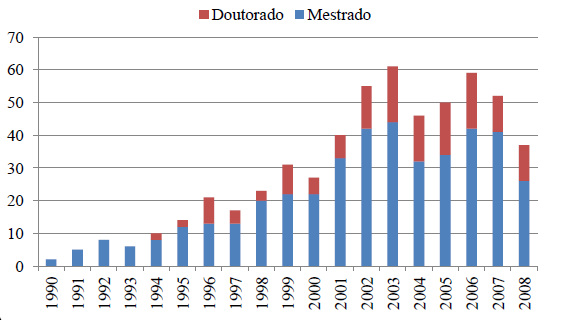
\includegraphics[scale=0.5]{figuras/figura-3}}
	}{
	\Fonte{os autores}
}
\end{figure}

Ou então figuras podem ser incorporadas de arquivos externos, como é o caso da \autoref{fig-grafico-1}. Se a figura que ser incluída se tratar de um diagrama, um gráfico ou uma ilustração que você mesmo produza, priorize o uso de imagens vetoriais no formato PDF. Com isso, o tamanho do arquivo final do trabalho será menor, e as imagens terão uma apresentação melhor, principalmente quando impressas, uma vez que imagens vetorias são perfeitamente escaláveis para qualquer dimensão. Nesse caso, se for utilizar o Microsoft Excel para produzir gráficos, ou o Microsoft Word para produzir ilustrações, exporte-os como PDF e os incorpore ao documento conforme o exemplo abaixo. No entanto, para manter a coerência no uso de software livre (já que você está usando LaTeX e abnTeX),  teste a ferramenta InkScape\index{InkScape}. ao CorelDraw\index{CorelDraw} ou ao Adobe Illustrator\index{Adobe! Illustrator}.  De todo modo, caso não seja possível  utilizar arquivos de imagens como PDF, utilize qualquer outro formato, como JPEG, GIF, BMP, etc.  Nesse caso, você pode tentar aprimorar as imagens incorporadas com o software livre \index{Gimp}Gimp. Ele é uma alternativa livre ao Adobe Photoshop\index{Adobe! Photoshop}.

\section{Usando Fórmulas Matemáticas}

\lipsum[2]

	\begin{equation}
		\begin{aligned}
			x = a_0 + \cfrac{1}{a_1
				+ \cfrac{1}{a_2
					+ \cfrac{1}{a_3 + \cfrac{1}{a_4} } } }
		\end{aligned}
	\end{equation}

\lipsum[3]

	\begin{equation}
		\begin{aligned}
			k_{n+1} = n^2 + k_n^2 - k_{n-1}
		\end{aligned}
	\end{equation}

\lipsum[4]

	\begin{equation}
		\begin{aligned}
			\cos (2\theta) = \cos^2 \theta - \sin^2 \theta
		\end{aligned}
	\end{equation}
	
\lipsum[5]

	\begin{equation}
		\begin{aligned}
			A_{m,n} =
			\begin{pmatrix}
			a_{1,1} & a_{1,2} & \cdots & a_{1,n} \\
			a_{2,1} & a_{2,2} & \cdots & a_{2,n} \\
			\vdots  & \vdots  & \ddots & \vdots  \\
			a_{m,1} & a_{m,2} & \cdots & a_{m,n}
			\end{pmatrix}
		\end{aligned}
	\end{equation}

\lipsum[6]

	\begin{equation}
		\begin{aligned}
			f(n) = \left\{ 
			\begin{array}{l l}
			n/2 & \quad \text{if $n$ is even}\\
			-(n+1)/2 & \quad \text{if $n$ is odd}
			\end{array} \right.
		\end{aligned}
	\end{equation}
	
\lipsum[7]

\section{Usando Algoritmos}

\lipsum[8]

\begin{algorithm}[h!]
	\SetSpacedAlgorithm
	\caption{\label{alg:algoritmo_de_colonica_de_formigas}Algoritmo de Otimização por Colônia de Formiga}
	\Entrada{Entrada do Algoritmo}
	\Saida{Saida do Algoritmo}
	\Inicio{
		Atribua os valores dos parâmetros\;
		Inicialize as trilhas de feromônios\;
		\Enqto{não atingir o critério de parada}{
			\Para{cada formiga}{
				Construa as Soluções\;
			}
			Aplique Busca Local (Opcional)\;
			Atualize o Feromônio\;
		}	
	}		
\end{algorithm}

\lipsum[9]

\section{Usando Código-fonte}

\lipsum[10]

\lstinputlisting[language=C++,caption={Hello World em C++}]{figuras/main.cpp}

\lipsum[11]

\begin{lstlisting}[language=Java,caption={Hello World em Java}]
public class HelloWorld {
	public static void main(String[] args) {
		System.out.println("Hello World!");
	}
}
\end{lstlisting}

\lipsum[11]

\section{Usando Teoremas, Proposições, etc}

Lorem ipsum dolor sit amet, consectetur adipiscing elit. Nunc dictum sed tortor nec viverra. consectetur adipiscing elit. Nunc dictum sed tortor nec viverra.

\begin{teo}[Pitágoras]
	Em todo triângulo retângulo o quadrado do comprimento da
	hipotenusa é igual a soma dos quadrados dos comprimentos dos catetos.
\end{teo}


Lorem ipsum dolor sit amet, consectetur adipiscing elit. Nunc dictum sed tortor nec viverra. consectetur adipiscing elit. Nunc dictum sed tortor nec viverra.

\begin{teo}[Fermat]
	Não existem inteiros $n > 2$, e $x, y, z$ tais que $x^n + y^n = z$
\end{teo}

Lorem ipsum dolor sit amet, consectetur adipiscing elit. Nunc dictum sed tortor nec viverra. consectetur adipiscing elit. Nunc dictum sed tortor nec viverra.

\begin{prop}
	Para demonstrar o Teorema de Pitágoras...
\end{prop}

Lorem ipsum dolor sit amet, consectetur adipiscing elit. Nunc dictum sed tortor nec viverra. consectetur adipiscing elit. Nunc dictum sed tortor nec viverra.

\begin{exem}
	Este é um exemplo do uso do ambiente exe definido acima.
\end{exem}

Lorem ipsum dolor sit amet, consectetur adipiscing elit. Nunc dictum sed tortor nec viverra. consectetur adipiscing elit. Nunc dictum sed tortor nec viverra.

\begin{xdefinicao}
	Definimos o produto de ...
\end{xdefinicao}

Lorem ipsum dolor sit amet, consectetur adipiscing elit. Nunc dictum sed tortor nec viverra. consectetur adipiscing elit. Nunc dictum sed tortor nec viverra.

\section{Usando Questões}


Lorem ipsum dolor sit amet, consectetur adipiscing elit. Nunc dictum sed tortor nec viverra. consectetur adipiscing elit. Nunc dictum sed tortor nec viverra.

\begin{questao}
	\item Esta é a primeira questão com alguns itens:
		\begin{enumerate}
			\item Este é o primeiro item
			\item Segundo item
		\end{enumerate}
	\item Esta é a segunda questão:
		\begin{enumerate}
			\item Este é o primeiro item
			\item Segundo item
		\end{enumerate}
	\item Lorem ipsum dolor sit amet, consectetur adipiscing elit. Nunc dictum sed tortor nec viverra. consectetur adipiscing elit. Nunc dictum sed tortor nec viverra.
		\begin{enumerate}
			\item consectetur
			\item adipiscing
			\item Nunc
			\item dictum
		\end{enumerate}
\end{questao}

\section{Citações}

\subsection{Documentos com três autores}

Quando houver três autores na citação, apresentam se os três, separados por ponto e vírgula, caso estes estejam após o texto. Se os autores estiverem incluídos no texto, devem ser separados por vírgula e pela conjunção "e".

\citeautoronline{tresautores}

\cite{tresautores}

\subsection{Documentos com mais de três autores}
Havendo mais de três autores, indica-se o primeiro seguido da expressão \textit{et al.} (do latim \textit{et alli}, que significa e outros), do ano e da página.

\citeautoronline{quatroautores}

\cite{quatroautores}

\cite{kurose2013}

\cite{pinheiro2004site}

\cite{costa1998}

\cite{gorshe2014ieee}

\citeautoronline{cartilhaUCAredessemfio}

\cite{moraes2014}

\cite{amer2016acm}

\cite{tanenbaum2013}

\cite{rodrigues2007site}

\cite{marconi2017}

\cite{gil2002}

\cite{barbosa2012}

\cite{wiki}

\subsection{Documentos de vários autores}

Havendo    citações    indiretas de    diversos    documentos    de    vários    autores, mencionados  simultaneamente e  que  expressam  a  mesma  ideia,  separam-se  os  autores  por ponto e vírgula, em ordem alfabética.

\cite{tresautores, quatroautores}

\section{Notas de Rodap\'{e}}

%Deve-se utilizar o sistema autor-data para as  citações no texto e o numérico para notas explicativas\footnote{Veja - se como exemplo desse tipo de abordagem o estudo de Netzer (1976)}. As notas de rodapé podem e devem ser alinhadas, a partir da segunda linha da mesma nota, abaixo da primeira letra da primeira palavra, de forma a destacar o expoente \footnote{Encontramos  esse  tipo  de  perspectiva  na  2ª  parte  do  verbete  referido  na  nota  anterior,  em  grande  parte  do estudo de Rahner (1962).} e sem espaço entre elas e com fonte menor (tamanho 10).


%	\chapter{Resultados}
\label{chap:resultados}

\lipsum[2]

\section{Resultados do Experimento A}
\label{sec:resultados-do-experimento-a}

\lipsum[3]

\section{Resultados do Experimento B}
\label{sec:resultados-do-experimento-b}

\lipsum[4]
%	\chapter{Conclusões e Trabalhos Futuros}
\label{chap:conclusoes-e-trabalhos-futuros}

\lipsum[2]
\lipsum[34]

\section{Contribuições do Trabalho}
\label{sec:contribuicoes-do-trabalho}

\lipsum[3]

\section{Limitações}
\label{sec:limitacoes}

\lipsum[4]

\section{Trabalhos Futuros}
\label{sec:trabalhos-futuros}

\lipsum[5]





	
	% Meu TCC
	\chapter{Introdução}
\label{cap:introducao}

\section{Contextualização}
\label{sec:contextualizacao}

Na década de 1970, o sistema Aloha\footnote{Originalmente, o sistema Aloha, desenvolvido por Norman Abramson em 1970, na Universidade do Havaí, funcionava como um protocolo para sistemas de comunicação via radiofrequência para o acesso remoto entre computadores enviando pacotes num sistema de radiocomunicação \cite{abramson1970acm,haykin2008}.} estabeleceu e operou uma rede de dados terrestres (AlohaNet) no estado americano do Havaí. O sistema usou um transponder acoplado em um satélite experimental da Agência Espacial Americana (NASA, do inglês, \textit{National Aeronautics and Space Administration}) (ATS-1) para demonstrar uma rede internacional de dados via satélite conectando a NASA, na Califórnia, e cinco universidades nos Estados Unidos, Japão e Austrália, fornecendo a primeira demonstração pública de uma rede de dados por pacotes sem fio \cite{abramson1970acm,SchwartzAbramson2009ieee}.

Mesmo com limitações como largura de banda e tecnologia de transmissão, foi graças ao pioneirismo do sistema Aloha, que as redes de comutação sem fio locais, conhecidas como LANs (do inglês, \textit{Local Area Network}) sem fio ou ainda WLANs (do inglês, \textit{Wireless Local Area Network}) surgiram como redes complementares às redes cabeadas tradicionais. Essa tecnologia de comunicação se desenvolveu devido a necessidade de implementação de um método alternativo de conexão que não privasse a movimentação do usuário durante a conexão com a rede. O tempo passou e a tecnologia evoluiu, deixou de ser restrita ao meio acadêmico e militar e se tornou acessível a empresas e ao usuário doméstico. Nos dias de hoje se pode pensar em redes \textit{wireless} (``sem fio'', em português) como uma alternativa bastante interessante em relação às redes cabeadas. Suas aplicações são muitas e variadas e o fato de ter a mobilidade como principal característica, tem facilitado a sua aceitação, principalmente nas empresas \cite{farias2005}.

Com o advento de \textit{notebooks}, \textit{tablets}, \textit{smartphones} e a promessa de acesso desimpedido à Internet global de qualquer hora e lugar por meio das comunicações sem fio, a demanda de acesso de dispositivos sem fio à Internet aumentou consideravelmente não só através da rede de telefonia móvel, agora plenamente possível, mas também por meio das redes Wi-Fi (do inglês, \textit{Wireless Fidelity}). O uso deste tipo de rede está se tornando cada vez mais comum, não só nos ambientes domésticos e corporativos, mas também em locais públicos (bares, lanchonetes, \textit{shoppings}, aeroportos, etc) e em instituições acadêmicas. Independentemente do crescimento futuro de equipamentos sem fio para Internet, já ficou claro que as redes sem fio e os serviços móveis relacionados que elas possibilitam se popularizaram e fazem parte do cotidiano das pessoas \cite{gast2002,kurose2013}.

Esse crescimento se deu, principalmente, com os avanços tecnológicos feitos na área, tornando a conexão mais rápida e confiável na troca de dados entre os nós da rede, fazendo com que os dispositivos móveis agregassem praticamente todas as funções que teria um computador de mesa convencional. Como consequência, estima-se que a força de trabalho móvel, em 2020, corresponderá a aproximadamente 1,75 bilhão de trabalhadores, segundo a Organização Internacional do Trabalho \cite{wba2017}. Para estes bilhões de usuários móveis, trabalhando dentro e fora do escritório tradicional, a mobilidade se tornou sinônimo de produtividade.

\textcolor{blue}{Segundo \citeonline{wba2017}, quando se trata de conexão sem fio com a Internet, os trabalhadores móveis preferem redes Wi-Fi ao invés de redes celulares, que são mais caras. Dessa forma, o Wi-Fi transporta mais da metade de todos os dados móveis de acordo com o Índice de Rede Visual da Cisco (VNI, do inglês, \textit{Visual Networking Index}) \cite{wba2017}.}

\section{Justificativa}
\label{sec:justificativa}

\textcolor{blue}{Os sistemas de telecomunicação utilizam cada vez mais as tecnologias sem fio.} Como resultado, as formas tradicionais de trabalho em rede no mundo mostraram-se inadequadas para enfrentar os desafios apresentados por nosso novo estilo de vida coletivo. Se os usuários precisarem estar conectados a uma rede por cabos físicos, seu movimento será drasticamente reduzido. A conectividade sem fio, no entanto, não apresenta esta restrição e permite muito mais movimento livre por parte do usuário da rede. Como consequência, as tecnologias sem fio estão invadindo o domínio tradicional das redes ``fixas'' ou ``com fio'' \cite{gast2002}.

As redes sem fio compartilham várias vantagens importantes. A vantagem mais evidente da rede sem fio é a mobilidade. Usuários de redes sem fio podem se conectar às redes existentes e, em seguida, podem circular livremente. Por exemplo, um usuário de telefone celular pode percorrer quilômetros no decorrer de uma única conversa desde que ele esteja coberto por alguma torre celular \cite{gast2002}.

%Da mesma forma, as redes Wi-Fi liberam os desenvolvedores de \textit{software} das amarras de um cabo Ethernet em uma mesa. Os desenvolvedores podem trabalhar na biblioteca, em uma sala de conferências, no estacionamento ou até mesmo na lanchonete do outro lado da rua. Enquanto os usuários sem fio permanecerem dentro do alcance do equipamento transmissor, eles poderão tirar proveito da rede \cite{gast2002}.

Em escolas e universidades, os laboratórios e bibliotecas estão quase sempre repletos de alunos que encontram na rede (Internet) uma boa fonte de consultas e pesquisas que complementam o conteúdo abordado em sala de aula, além de facilitar a comunicação e a troca de informações entre os estudantes. Graças à tecnologia de comunicação sem fio Wi-Fi, estudantes e professores não dependem exclusivamente dos laboratórios de informática para se conectarem à Internet.

O acesso sem fio pode ser disponibilizado por todo o ambiente educacional, bastando apenas o usuário ligar seu \textit{notebook} ou dispositivo móvel de qualquer local com cobertura e estabelecer a conexão com a rede.

%Outra propriedade benéfica das redes sem fio é que estas geralmente têm muita flexibilidade, o que pode se traduzir em implantação rápida. Redes sem fio usam um número de estações base para conectar usuários a uma rede existente. O lado da infraestrutura de uma rede sem fio, no entanto, é qualitativamente o mesmo, esteja conectando um usuário ou um milhão de usuários. Para oferecer serviço em uma determinada área, é necessário a presença de estações base e antenas no lugar.

%Uma vez que essa infraestrutura é construída, adicionar um usuário a uma rede sem fio é principalmente uma questão de autorização. Com a infraestrutura disponível, ela deve ser configurada para reconhecer e oferecer serviços aos novos usuários, mas a autorização não exige mais infraestrutura. Adicionar um usuário a uma rede sem fio é uma questão de configurar a infraestrutura, mas isso não envolve a passagem de cabos, o fechamento de terminais e a aplicação de correções em um conector \cite{gast2002}.

%Este exemplo simples ignora os desafios de escalabilidade. Naturalmente, se os novos usuários sobrecarregarem a infraestrutura existente, a própria infraestrutura precisará ser reforçada para que mais usuários possam ser conectados. A expansão da infraestrutura pode ser cara e demorada, especialmente se envolver aprovação legal e regulatória de faixas de frequência. No entanto, o ponto básico é válido: adicionar um usuário a uma rede sem fio pode ser reduzido a uma questão de configuração, enquanto adicionar um usuário a uma rede fixa requer conexões físicas \cite{gast2002}.

%Embora seja possível atender a um grupo fluido de usuários com conectores padrão Ethernet, o fornecimento de acesso através de uma rede com fio é problemático por vários motivos. A passagem de cabos é demorada, cara e também pode exigir adaptações no espaço físico; determinar corretamente o número de enlaces de cabos é difícil devido ao intenso fluxo de pessoas. Com uma rede sem fio, porém, não há necessidade de eventuais alterações na construção ou fazer suposições estatísticas complexas sobre a demanda. Uma infraestrutura com fio simples se conecta à Internet e, em seguida, a rede sem fio pode acomodar quantos usuários forem necessários \cite{gast2002}.

%Apesar das várias vantagens oferecidas pelas redes sem fio, as mesmas não substituem as LANs cabeadas. Servidores e outros equipamentos de \textit{datacenter} devem acessar dados, mas a localização geográfica do servidor é irrelevante. A velocidade das redes sem fio é limitada pela largura de banda disponível. A teoria da informação pode ser usada para deduzir o limite da velocidade de uma rede. A menos que as autoridades reguladoras estejam dispostas a aumentar as bandas de espectro não licenciadas, há um limite superior na velocidade das redes sem fio. O \textit{hardware} de rede sem fio tende a ser mais lento que o \textit{hardware} com fio. Diferentemente do padrão Ethernet, os padrões de rede sem fio devem avaliar cuidadosamente os quadros de entrada para proteger contra perda devido à falta de confiabilidade do meio \textit{wireless} \cite{gast2002}.

Para quantificar a relevância das redes \textit{wireless}, em 2022, 51\% do tráfego de dados móveis global será transportado pela redes Wi-Fi segundo a Cisco VNI no ano de 2018. No Brasil, 48\% do tráfego de dados total da Internet será movido através das redes Wi-Fi de acordo com as estimativas disponibilizadas também pela Cisco VNI em 2018.

Para que haja transferência de dados, as redes sem fio usam ondas de rádio como meio de transmissão, entretanto essa abordagem apresenta vários desafios. As ondas de rádio podem sofrer vários problemas de propagação que podem interromper o \textit{link} de rádio, como interferência, perdas de multipercurso e áreas de sombra (locais sem cobertura de sinal), que podem atenuar a potência do sinal Wi-Fi, reduzindo, por consequência, a taxa de transferência e a qualidade da conexão, assim como a viabilidade de alguns serviços que exigem um limite mínimo destes recursos para funcionar com eficiência
 \cite{gast2002}. Isso significa que o canal de rádio impõe limitações fundamentais para o desempenho dos sistemas de comunicação sem fio.
 
Devido ao amplo crescimento e ao alto interesse pela criação de ambientes com mobilidade no acesso à rede em instituições públicas e também no mercado privado, torna-se essencial um estudo aprofundado na área ao planejar ou avaliar novas instalações, sempre buscando qualidade, confiabilidade e respeito às normas técnicas e legislação vigente.

% Proposta do trabalho
Para que uma WLAN tenha um desempenho satisfatório aos seus usuários, vários fatores devem ser levados em consideração para que o processo de instalação corresponda o mais fielmente possível ao planejado. Um método amplamente utilizado por projetista de redes, seja cabeada ou sem fio, é o \textit{site survey}. O \textit{site survey} é um conjunto de métodos de análise detalhada da estrutura do local onde será implantada a nova rede ou aplicada a uma infraestrutura já existente com o objetivo de identificar e solucionar problemas no sistema \cite{pinheiro2004site}.

Portanto, a proposta deste trabalho consiste em analisar a infraestrutura geral da rede sem fio do Bloco Didático do IFCE \textit{campus} Tauá a fim de avaliar se a configuração atual da rede sem fio provê um serviço satisfatório baseado na análise dos mapas de calor dos sinais de rádio da área.

Mediante o exposto, nesta proposta de trabalho será empregado a técnica de projeto chamada \textit{site survey} para levantar dados do Bloco Didático, especialmente sobre como ocorre a propagação dos sinais e medir o nível de sinal da rede sem fio, a partir dos pontos de acesso já presentes no local, pois estes são aspectos de grande impacto no desempenho das redes sem fio em geral.  Este método tem como intuito detectar possíveis problemas que incapacite a rede de prover a cobertura necessária para que serviços básicos (pesquisas, estudos, experimentos, etc.) dos estudantes, docentes e servidores sejam atendidas com o mínimo de satisfação.

É extremamente recomendado aliar ao \textit{site survey} ferramentas complementares para auxiliar o processo de inspeção do local, como, por exemplo, um \textit{software} adequado instalado em um \textit{notebook} que possa realizar a medição de potência do sinal e também identificar o canal de frequência em que opera as redes vizinhas, com objetivo de identificar possíveis interferências destrutivas no sinal.

Depois de fazer uso da ferramenta apropriada para a análise, é importante identificar o ambiente de trabalho para determinar a localização dos equipamentos e analisar o desempenho da rede Wi-Fi, para garantir uma melhor cobertura e prestar um melhor serviço.

Com os resultados se buscará simular o grau de eficiência da infraestrutura de rede sem fio ofertada pelo IFCE Tauá ao Bloco Didático, propor uma solução para conseguir um melhor desempenho através de recomendações para otimizar o serviço de rede \textit{wireless}.

\section{Objetivos}
\label{sec:objetivos}

Este trabalho apresenta como objetivo geral mostrar a aplicação da metodologia \textit{site survey} para análise de cobertura e recepção do sinal Wi-Fi no Bloco Didático do Instituto Federal do Ceará \textit{campus} Tauá.
Já com relação aos objetivos específicos, este trabalho visa:
\begin{compactitem}
	\item Analisar a infraestrutura atual da rede sem fio do Bloco Didático através de sua planta estrutural;
	\item Identificar e localizar os locais de concentração dos pontos de acesso para a elaboração de plantas, desenhos ou esquemáticos;
	\item Verificar a presença de possíveis obstáculos, fontes de interferência e áreas de sombra que possam limitar a propagação do sinal da rede sem fio;
	\item Coletar dados em campo do Bloco Didático a respeito da propagação do sinal da rede Wi-Fi;
	\item Sugerir uma melhoria para a rede com base nos resultados obtidos.
\end{compactitem}

\section{Organização do Trabalho}
\label{sec:organnizacao-do-trabalho}

Este trabalho está dividido da seguinte forma:

\begin{compactitem}
	\item Capítulo 2: aborda os principais conceitos por trás do processo de transmissão em redes sem fio, essenciais para a compreensão do funcionamento geral das comunicações sem fio, incluindo os mecanismos básicos da propagação de ondas eletromagnéticas e alguns modelos de propagação utilizados na predição de enlaces de rádio, tanto para ambientes internos quanto para ambientes externos.
	
	\item Capítulo 3: apresenta as principais características das redes Wi-Fi, a sua arquitetura, o padrão IEEE 802.11 (o qual as redes Wi-Fi são estruturadas) e, por fim, o método de inspeção \textit{site survey} como ferramenta para o planejamento e avaliação de redes \textit{wireless}.
	
	\item Capítulo 4: apresenta um estudo de caso realizado a partir da aplicação do \textit{site survey} na infraestrutura de rede sem fio do Bloco Didático do Instituto Federal de Educação, Ciência e Tecnologia do Ceará \textit{campus} Tauá; Expõe e discute os resultados obtidos ao fim do processo de coleta de dados do local alvo; Propõe medidas de intervenção na infraestrutura da rede para a melhoria da cobertura do sinal nos dois andares analisados.
	
	\item Capítulo 5: apresenta o encerramento do trabalho baseado no conteúdo discutido e nos resultados obtidos no estudo de caso.
\end{compactitem}
	\chapter{Transmissão em Redes sem Fio}
\label{cap:transmissao-redes-sem-fio}

As ondas de rádio são fáceis de gerar, podem percorrer longas distâncias e penetrar em diversos tipos de materiais, por isso, são amplamente utilizadas para comunicação, desde ambientes abertos até ambientes fechados. As ondas de rádio também são omnidirecionais, o que significa que elas se propagam em todas as direções a partir da origem. Desse modo, o transmissor e o receptor não precisam estar perfeitamente alinhados para que haja comunicação \cite{tanenbaum2011}. Por todas essas características, as ondas de rádio são o principal recurso para que a comunicação sem fio se tornasse possível, resultando em sua dispersão generalizada pelo globo.

\section{O Espectro Eletromagnético}
\label{sec:espectro-eletromagnetico}

Quando se movem, os elétrons criam ondas eletromagnéticas que podem se propagar pelo espaço livre (até mesmo no vácuo), transportando energia durante o percurso. Essas ondas foram previstas pelo físico inglês James Clerk Maxwell em 1865 e foram observadas pela primeira vez pelo físico alemão Heinrich Hertz em 1887 \cite{tanenbaum2011}.

O número de ondas completas que passam por um ponto fixo dentro de um período de tempo é chamado de frequência, e é medido em Hertz (Hz, em homenagem a Heinrich Hertz). A distância entre dois pontos máximos (ou mínimos) consecutivos é chamada comprimento de onda, designada universalmente pela letra grega $\lambda$ (lambda). A \autoref{fig:onda} ilustra essa propriedade das ondas.

A velocidade de uma onda qualquer depende do meio em que ela se propaga. No vácuo, todas as ondas eletromagnéticas viajam na mesma velocidade, a da luz, que é aproximadamente igual a $3 \times 10^8$ m/s, independentemente de sua frequência \cite{tanenbaum2011}.

Essas três grandezas -- frequência ($f$), comprimento de onda ($\lambda$) e velocidade ($c$) -- se relacionam (no vácuo) através da seguinte expressão:

\begin{equation}
	\begin{aligned}
		c = \lambda f
	\end{aligned}
\end{equation}

Desta forma, pode-se observar que as propriedades de uma onda eletromagnética dependem de sua frequência (ou comprimento de onda), já que a velocidade da luz é uma constante.

\begin{figure}[H]
	\centering
	\Caption{\label{fig:onda}Propriedades de uma onda.}	
	\UECEfig{}{
		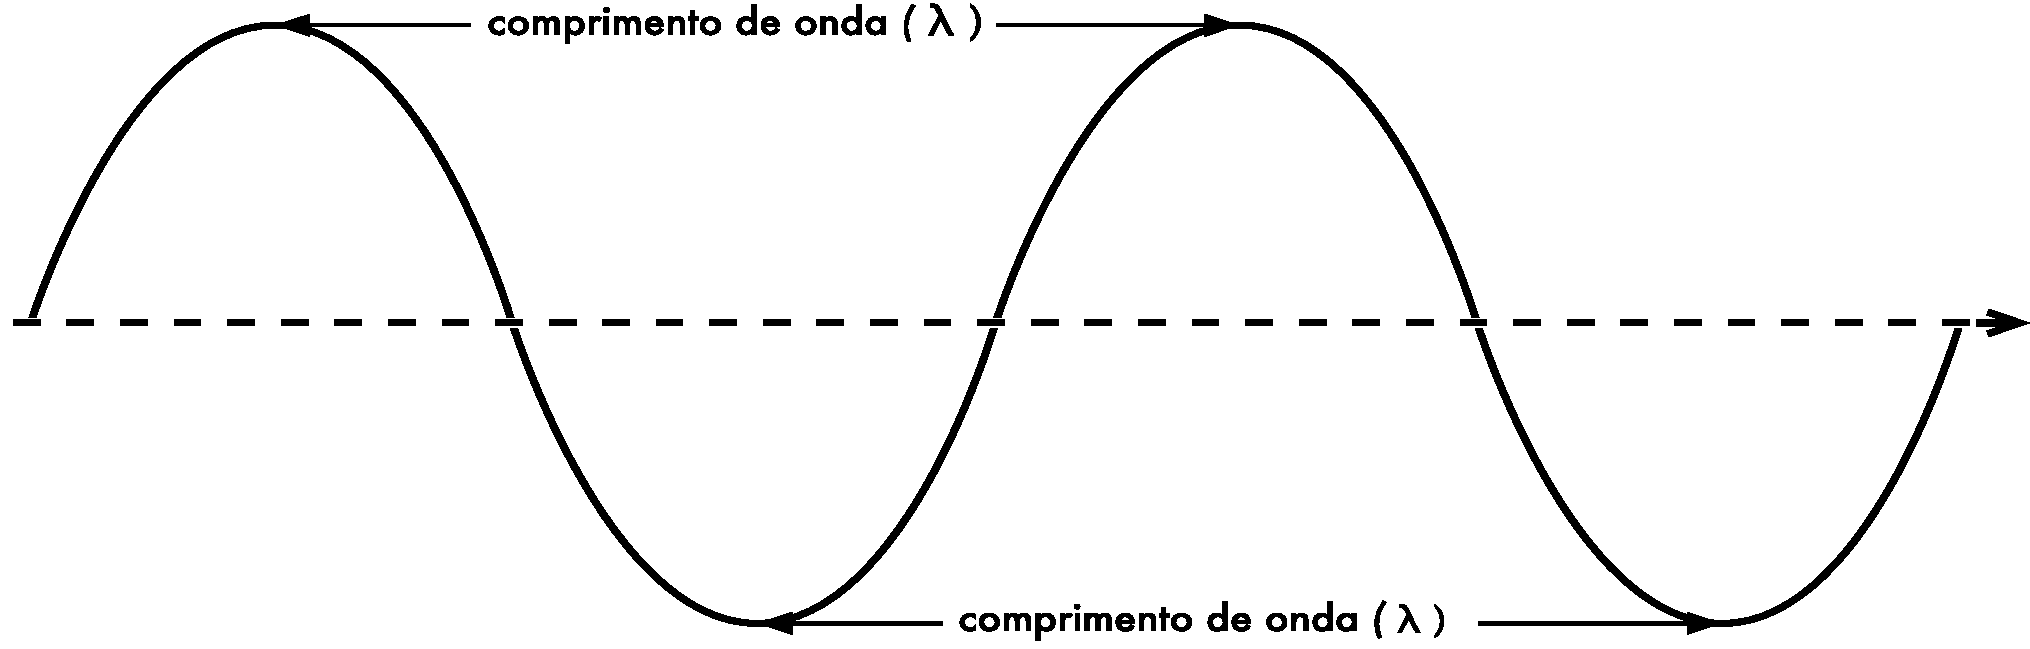
\includegraphics[scale=.4]{figuras/onda_wave.pdf}
	}{
		\Fonte{\citeonline[p. ~10]{flickenger2008}.}
	}	
\end{figure}

Uma onda eletromagnética pode ser gerada ou captada por circuitos eletrônicos simples. Além disso, esse tipo de onda se propaga no vácuo, o que permite a comunicação entre antenas terrestres com satélites no espaço e vice-versa, entre os próprios satélites e entre dois pontos localizados em qualquer parte da superfície terrestre \cite{fluminense2010}.

Os dispositivos sem fio usam ondas eletromagnéticas para transmitir suas informações, porém são restritos para operar em uma determinada banda (ou faixa) de frequência. Cada faixa tem uma largura de banda associada, que é simplesmente a quantidade de espaço de frequência na banda. Se a variação entre 2,40 GHz e 2,48 GHz é usada por um dispositivo, então a largura de banda será de 0,08 GHz ou 80 MHz.

A largura de banda adquiriu uma conotação de ser uma medida da capacidade de dados de um \textit{link}. Uma grande quantidade de matemática, teoria da informação e processamento de sinais pode ser usada para demonstrar que fatias mais largas de frequência podem ser usadas para transmitir mais informações \cite{gast2002}. Por exemplo, um canal de telefonia móvel analógico requer uma largura de banda de 20 kHz. Os sinais de televisão são muito mais complexos, já que, necessariamente, transmitem tráfego de áudio e vídeo, e por esse motivo possuem uma largura de banda consideravelmente maior, cerca de 6 MHz \cite{gast2002}.

Cada banda de frequência utilizada nas telecomunicações estão contidas em um modelo de escala comum, onde é apresentado o intervalo completo de todas as possíveis frequências da radiação eletromagnética, denominado de espectro eletromagnético. A \autoref{fig:espectro} ilustra todas as variações de frequências contidas no espectro eletromagnético.

\begin{figure}[H]
	\centering
	\Caption{\label{fig:espectro}O espectro eletromagnético e a maneira como ele é usado na comunicação.}	
	\UECEfig{}{
		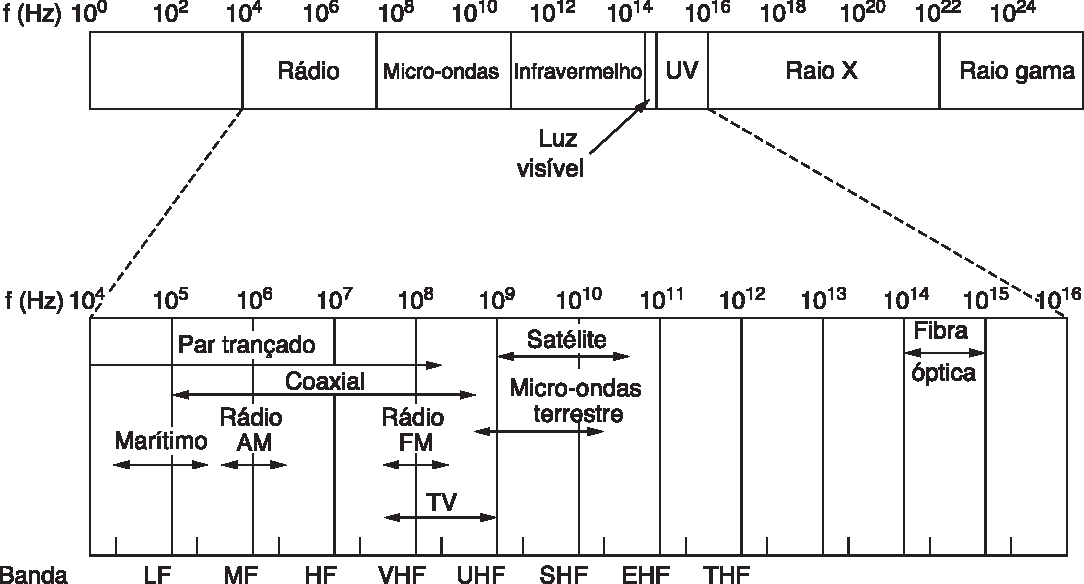
\includegraphics[scale=1]{figuras/espectro_eletromagnetico.pdf}
	}{
		\Fonte{\citeonline[p. ~70]{tanenbaum2011}.}
	}	
\end{figure}

\begin{citacao}
	As faixas de rádio, microondas, infravermelho e luz visível do espectro podem ser usadas na transmissão de informações, por meio de modulação da amplitude, da frequência ou da fase das ondas. A luz ultravioleta, os raios X e os raios gama representariam opções ainda melhores, por terem frequências mais altas, mas são difíceis de produzir e modular, além de não se propagarem bem através dos prédios e de serem perigosos para os seres vivos \cite[p.~65]{tanenbaum2011}.
\end{citacao}

O uso de uma faixa de frequência é rigorosamente controlado pelas autoridades reguladoras através de processos de licenciamento. No âmbito mundial, o processo de padronização de alocação de frequências para uso específico é realizado pela União Internacional de Telecomunicações (ITU, do inglês, \textit{International Telecommunication Union}). No Brasil, a ANATEL (Agência Nacional de Telecomunicações) representa a entidade responsável pela definição e fiscalização da utilização das faixas de frequência em território nacional. Essas determinações regulatórias visam coibir o uso das faixas de frequência sem permissão por infratores como estações de rádio e TVs piratas.

Entretanto, existem faixas de frequência que não estão sujeitas a autorização de uso pelos órgãos reguladores, ou seja, são bandas de frequência abertas para transmitir. Essas frequências não licenciadas são conhecidas como ISM (do inglês, \textit{Industrial, Scientific, Medical}). As bandas ISM foram padronizadas na maioria dos países em três faixas de frequência: 900 MHz, 2.4 GHz e 5 GHz \cite{moraes2010,tanenbaum2011}. A \autoref{fig:ism_unii} exibe a alocação das frequências ISM e também das bandas U-NII (do inglês, \textit{Unlicensed National Information Infrastructure}).

\begin{figure}[H]
	\centering
	\Caption{\label{fig:ism_unii}As bandas ISM e U-NII.}	
	\UECEfig{}{
		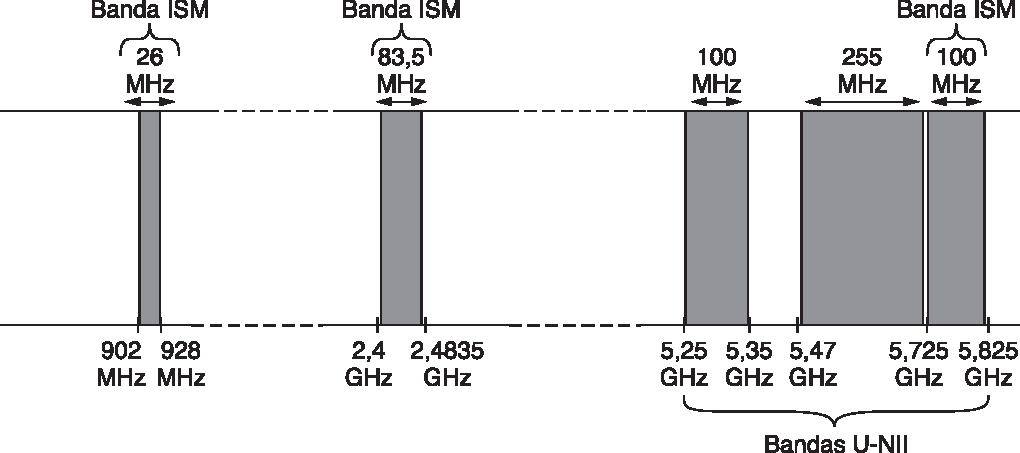
\includegraphics[scale=.64]{figuras/ism-unii.pdf}
	}{
		\Fonte{\citeonline[p. ~66]{tanenbaum2011}.}
	}	
\end{figure}

\section{Efeitos de Propagação em Ondas Eletromagnéticas}
\label{sec:efeitos-propagacao-OE}

Sistemas de comunicações sem fio utilizam-se de ondas eletromagnéticas para o envio de sinais através do ar. Na perspectiva de um usuário, conexões sem fio não são particularmente diferentes de qualquer outro tipo de conexão de rede: os serviços de transmissão de informações funcionarão de acordo com o esperado \cite{flickenger2008}. Mas ondas de rádio possuem algumas propriedades inesperadas se comparadas com o meio guiado.  Por exemplo: é muito fácil ver o caminho que o cabo Ethernet faz, só é preciso seguí-lo em sua extensão. Também pode-se ter a confiança de que ter vários cabos Ethernet lado a lado não causarão problemas, uma vez que os sinais trafegam no interior dos fios.

Diferentemente dos enlaces físicos, o caminho de uma onda de rádio entre transmissor e receptor pode variar de uma simples linha de visão completamente desobstruída até um cenário em que seja obstruído por prédios, terrenos elevados e áreas de vegetação densa \cite{rappaport2009}. Isso quer dizer que os sinais de rádio são aleatórios e de difícil análise. Até a velocidade do deslocamento dos terminais influencia na rapidez com que o sinal enfraquece \cite{rappaport2009}.

Portanto, o estudo da propagação dos sinais de radiofrequência é importante para a compreensão das comunicações sem fio porque fornece a modelagem física necessária, o que resulta em uma boa estimativa de potência requerida para o estabelecimento do enlace de comunicação para que haja comunicação confiável \cite{haykin2008}. Além disso, o estudo da propagação auxilia na compreensão das técnicas de recepção para compensação das perdas introduzidas pela transmissão sem fio \cite{haykin2008}.

Os efeitos sofridos pela onda eletromagnética ao se propagar são diversos, mas os principais são a absorção, a reflexão, a difração, a refração, o desvanecimento e a interferência \cite{flickenger2008,haykin2008,rappaport2009}.

\subsection{Absorção}
\label{sub:absorcao}

Quando ondas eletromagnéticas penetram algum objeto, elas geralmente atenuam ou dissipam-se totalmente, como ilustra a \autoref{fig:absorcao}. O quanto elas perdem de potência irá depender de sua frequência e do material em que penetram \cite{flickenger2008}.

\begin{figure}[H]
	\centering
	\Caption{\label{fig:absorcao}Atenuação de uma onda devido a absorção.}	
	\UECEfig{}{
		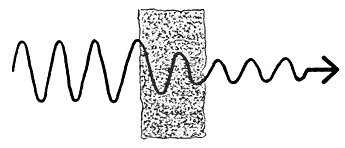
\includegraphics[scale=.75]{figuras/absorcao1.png}
	}{
		\Fonte{Adaptado de \citeonline{megasorber2019c}.}
	}
\end{figure}

Para ondas de rádio, os dois principais materiais absorventes são \cite{flickenger2008}:

\begin{compactitem}
	\item metais: elétrons podem mover-se livremente em metais, sendo prontamente capazes de oscilar e absorver a energia de uma onda que incida sobre eles.
	\item água: ondas de rádio fazem com que as moléculas de água agitem-se, tomando parte da energia da onda.
\end{compactitem}

\subsection{Reflexão}
\label{sub:reflexao}

Nas comunicações sem fio terrestres, normalmente não existe uma linha de visada desimpedida no percurso do sinal de rádio entre transmissor e receptor e as comunicações geralmente envolvem o fenômeno da reflexão \cite{haykin2008}. O fenômeno da reflexão de ondas eletromagnéticas é mostrado na \autoref{fig:reflexao}.

``A reflexão ocorre quando uma onda eletromagnética em propagação colide com um objeto que possui dimensões muito grandes em comparação com o comprimento de onda da onda que se propaga'' \cite[p.~76]{rappaport2009}.

\begin{figure}[H]
	\centering
	\Caption{\label{fig:reflexao}Reflexão de ondas de rádio.}	
	\UECEfig{}{
		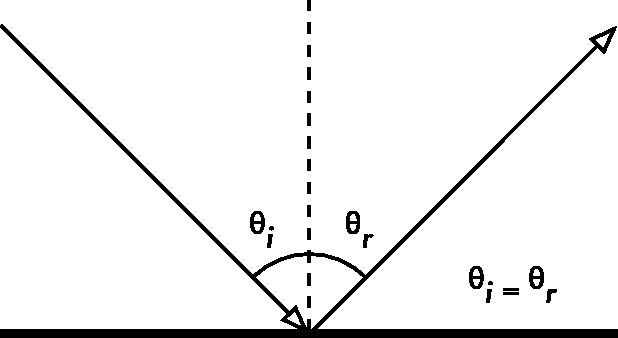
\includegraphics[scale=.72]{figuras/reflexao.pdf}
	}{
		\Fonte{\citeonline[p. ~18]{flickenger2008}.}%
		\Nota{O ângulo de incidência ($\theta_i$) é igual ao ângulo de reflexão ($\theta_r$).}%
	}
\end{figure}

\subsubsection{Multipercurso}
\label{subsec:multipercurso}

Ainda que as regras de reflexão sejam relativamente simples, a situação se torna mais complexa por espalhamento das ondas eletromagnéticas ao chocarem-se contra a superfície das construções e objetos ao redor, como pode ser visto na \autoref{fig:multipath} \cite{haykin2008}.  Esses percursos de propagação múltiplos são conhecidos como multipercurso ou multicaminho. Até mesmo quando existe uma linha de visão direta, o multipercurso ainda ocorre devido às reflexões no solo e nas estruturas próximas a estação móvel \cite{rappaport2009}.

\begin{figure}[H]
	\centering
	\Caption{\label{fig:multipath}Sinais refletidos geram o multipercurso.}	
	\UECEfig{}{
		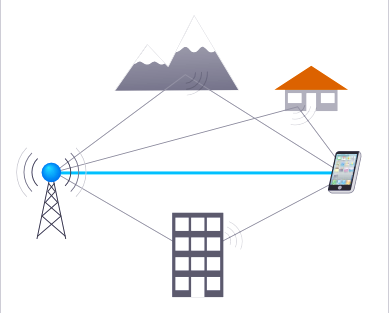
\includegraphics[scale=.8]{figuras/Multipath1.png}
	}{
		\Fonte{Adaptado de \citeonline{yatebts2015}.}
	}
\end{figure}

\subsection{Difração}
\label{sub:difracao}

O fenômeno da difração está relacionado ao fato de as ondas eletromagnéticas contornarem objetos quando passam ao redor dos mesmos, tais como arestas de construções ou picos de montanhas (\autoref{fig:difracao}) ou quando atravessam barreiras contendo aberturas. Para altas frequências, a difração, assim como a reflexão, depende do formato do objeto, além da amplitude, fase e polarização da onda incidente sobre o ponto difrator \cite{rappaport2009}.

\begin{figure}[H]
	\centering
	\Caption{\label{fig:difracao}Difração no topo de uma montanha.}	
	\UECEfig{}{
		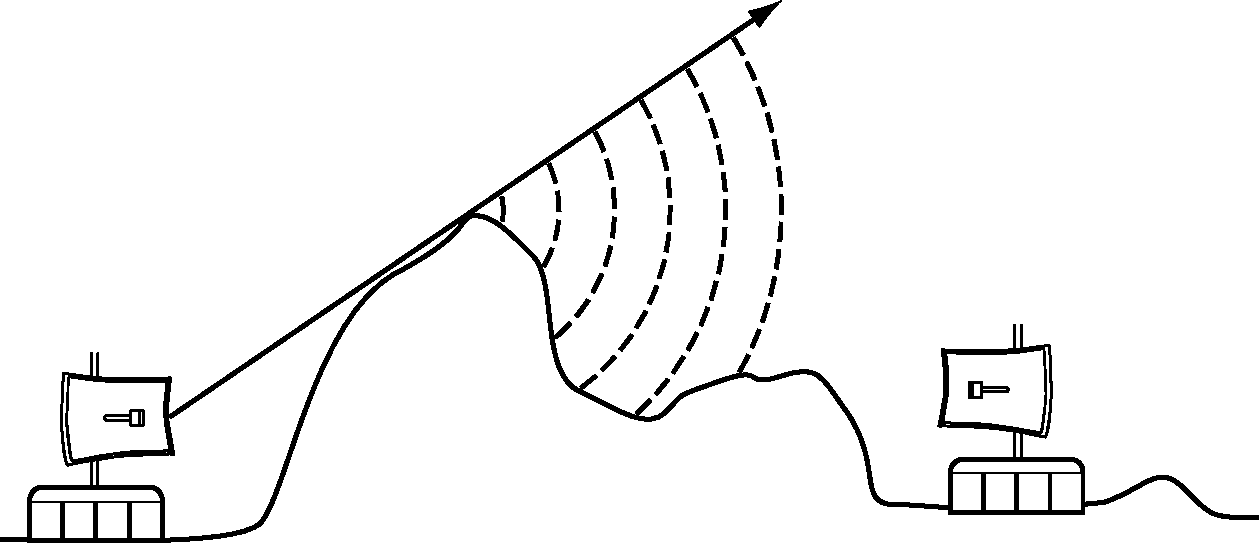
\includegraphics[scale=.6]{figuras/difracao1.pdf}
	}{
		\Fonte{\citeonline[p. ~20]{flickenger2008}.}
	}
\end{figure}

Vale ressaltar que a difração ocorre ao custo de perda de potência, isto é, a energia da onda difratada é significativamente menor que a da onda original. Mas ainda sim existe, nas ondas secundárias resultantes, força suficiente para produzir um sinal útil, além da vantagem da difração para contornar obstáculos entre transmissor e receptor \cite{flickenger2008,rappaport2009}.

\subsection{Refração}
\label{sub:refracao}

A refração ocorre quando as ondas eletromagnéticas mudam a trajetória de propagação quando passam de um meio para outro, assim como mostra a \autoref{fig:refracao}. Na transição, o nível de energia da onda é reduzido, pois uma fração da onda é refletida \cite{flickenger2008}. Um exemplo de refração ocorre quando a luz, propagando-se no ar, encontra uma interface com a água. A utilização da refração nas comunicações sem fio fica limitada a circunstâncias especiais, tais como comunicações via satélite, pois a transmissão necessita penetrar através das camadas da atmosfera, cada uma com densidade distinta da outra \cite{rappaport2009}.

\begin{figure}[H]
	\centering
	\Caption{\label{fig:refracao}Refração.}	
	\UECEfig{}{
		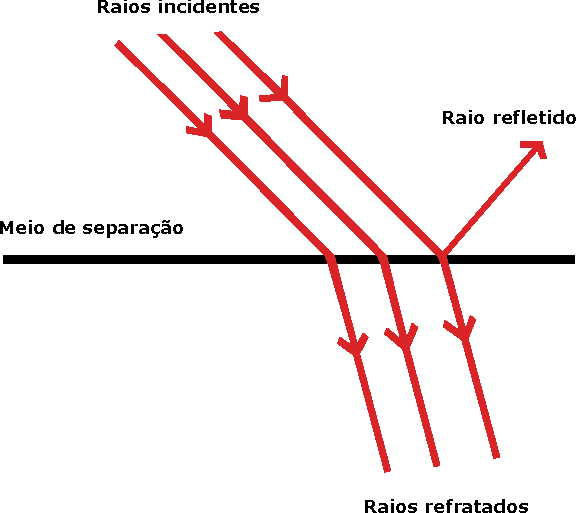
\includegraphics[scale=.69]{figuras/refracao.pdf}
	}{
		\Fonte{Adaptado de \citeonline{teixeira2019c}.}
	}
\end{figure}

\subsection{Interferência}
\label{sub:interferencia}

Interferência é o fenômeno que corrompe um sinal enquanto ele viaja em um enlace da origem para o destino. A perturbação pode interromper, obstruir, degradar ou limitar a recepção efetiva de sinais. Esses efeitos podem variar de uma simples degradação de dados a uma perda total de dados. O termo é frequentemente usado para se referir à adição de sinais indesejados a um sinal útil \cite{flickenger2008}.

Em comunicações sem fio, a interferência é causada principalmente por fontes de radiofrequência que operam na mesma faixa de frequência, como por exemplo, o aparelho de microondas e as redes 802.11 (detalhadas no capítulo 3), ambas operando na banda de 2.4 GHz \cite{moraes2010}. A \autoref{fig:interferencia} mostra um exemplo de interferência entre ondas de rádio.
\begin{figure}[H]
	\centering
	\Caption{\label{fig:interferencia}Interferência entre ondas de rádio.}	
	\UECEfig{}{
		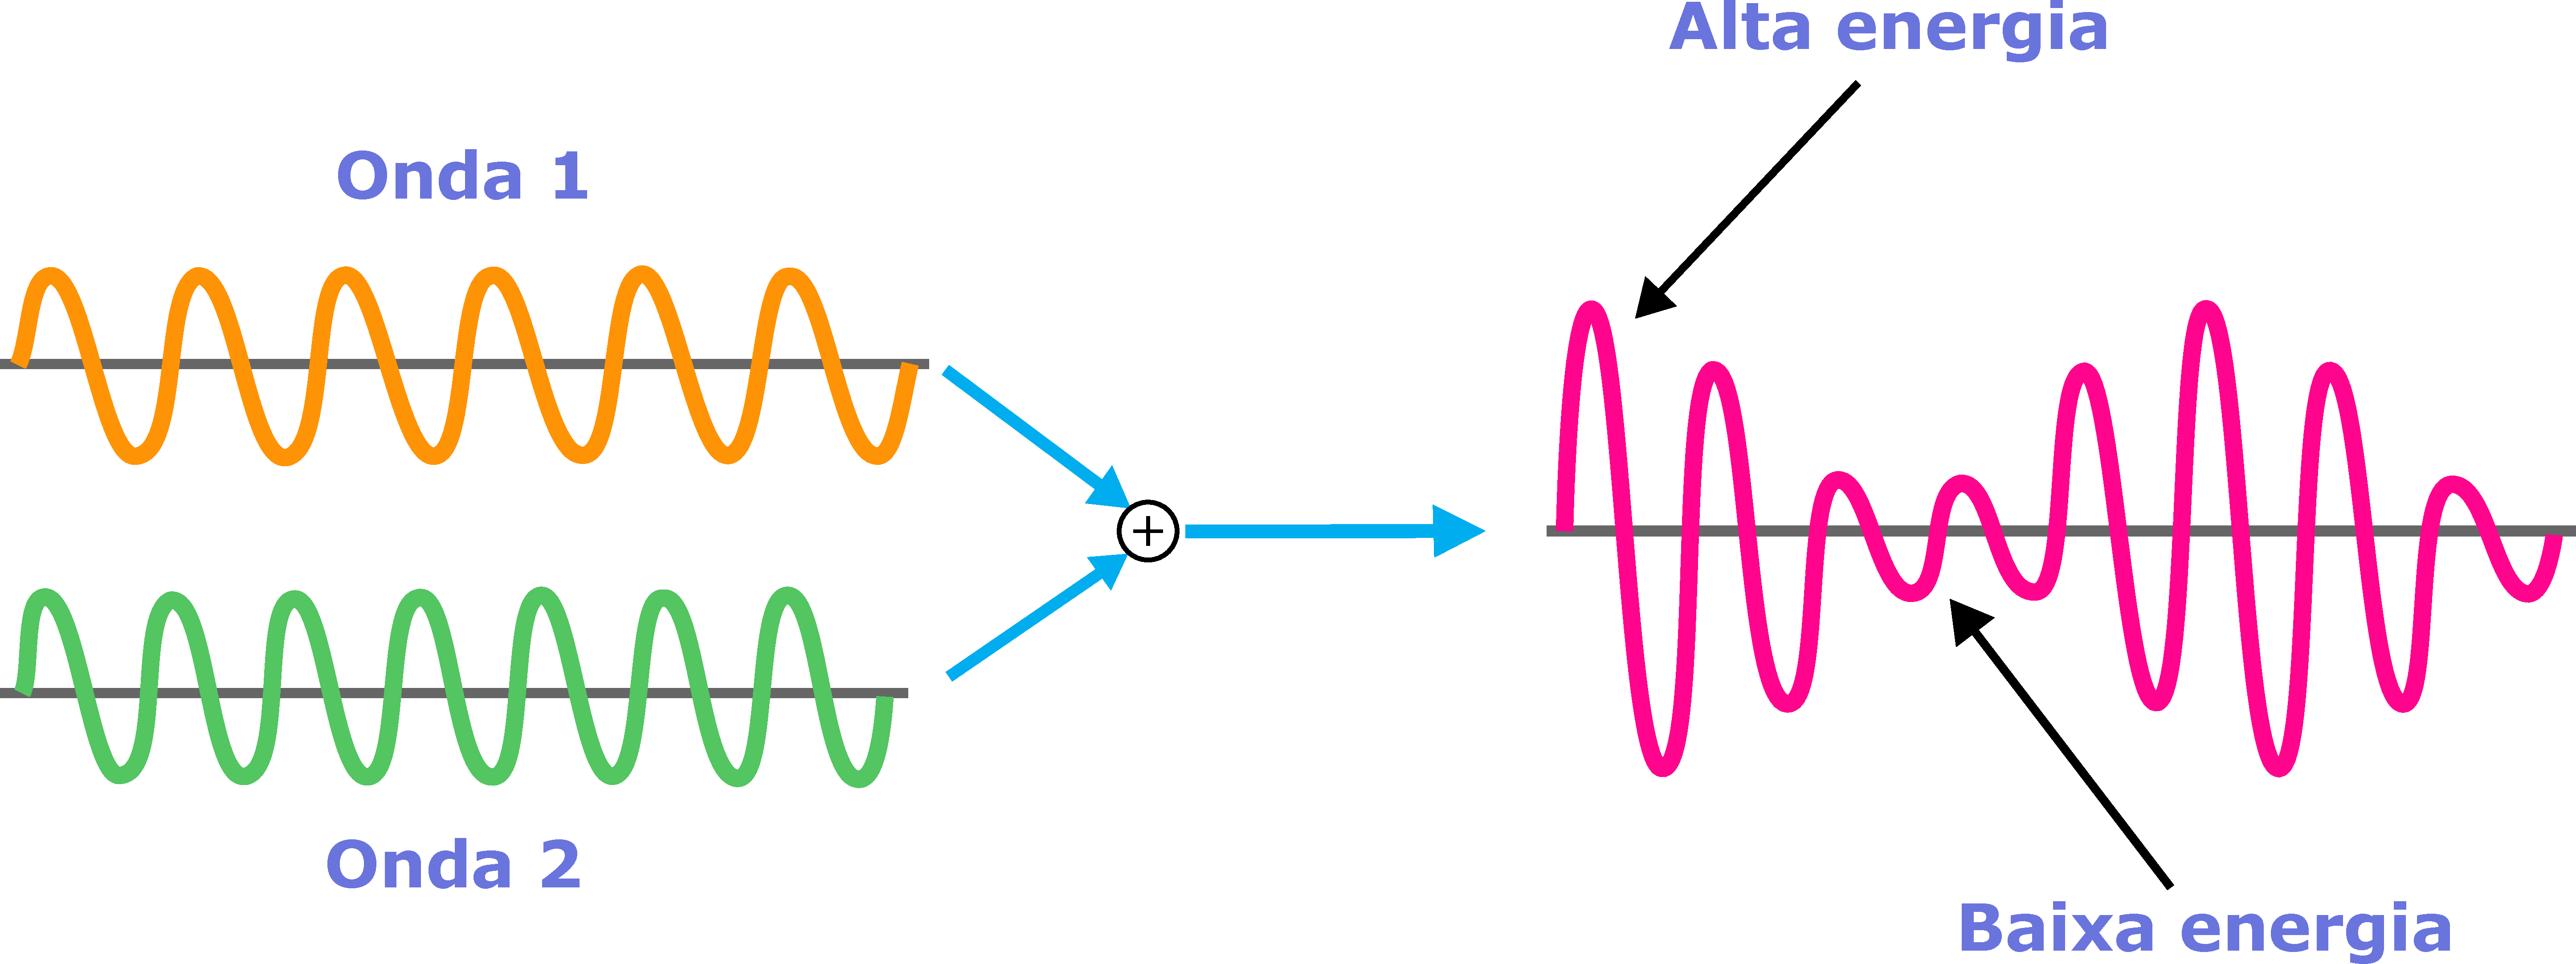
\includegraphics[scale=.13]{figuras/interferenciaSVG_pdf.pdf}
	}{
		\Fonte{Adaptado de \citeonline{physics2015}.}
	}
\end{figure}

\subsection{Desvanecimento (\textit{fading})}
\label{sub:desvanecimento}

O desvanecimento é um fenômeno causado pela variabilidade da intensidade do sinal no tempo associado à mobilidade da estação móvel \cite{haykin2008,rappaport2009}. Frequentemente, o sinal recebido é uma combinação de vários modos de propagação resultantes da reflexão e da difração. Assim, a maior parte da comunicação acontece por espalhamento das ondas eletromagnéticas, que chegam de diferentes direções com diferentes atrasos de propagação \cite{haykin2008}. No receptor, o sinal final é a soma vetorial dessas ondas de caminhos múltiplos, podendo interagir umas com as outras construtiva ou destrutivamente (\autoref{fig:fading}), dependendo da amplitude e da fase de cada componente espectral \cite{haykin2008}.

\begin{figure}[H]
	\centering
	\Caption{\label{fig:fading}Interferência construtiva e destrutiva.}	
	\UECEfig{}{
		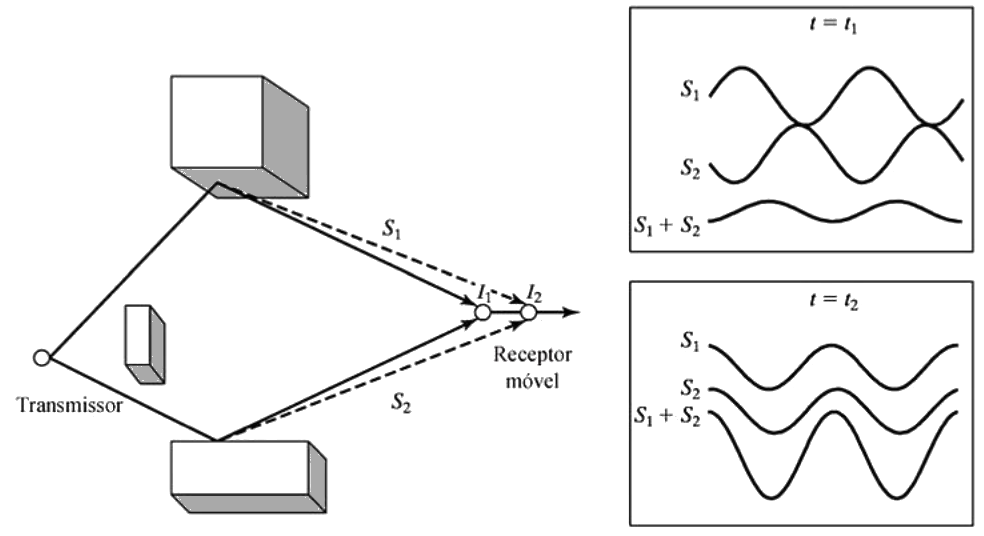
\includegraphics[scale=.35]{figuras/inter.png}
	}{
		\Fonte{\citeonline[p. ~57]{haykin2008}}
	}
\end{figure}

A rapidez com que as flutuações na intensidade do sinal ocorre pode ser classificada como desvanecimento lento (\textit{slow-fading}) ou desvanecimento rápido (\textit{fast-fading}), como ilustra a \autoref{fig:fading-slow-fast} \cite{haykin2008}.

O desvanecimento lento origina-se devido ao efeito da mobilidade do terminal do usuário. É o resultado de mudança de caminho (reflexões) de sinal devido a obstruções como árvores ou edifícios distantes do receptor. O movimento relativo da estação móvel em relação a esses objetos é pequeno, o que resulta em uma perda de percurso pequena \cite{haykin2008}.

O desvanecimento rápido surge devido a alternância nos modos de interferência construtiva e destrutiva causados por multipercurso, juntamente com a velocidade de deslocamento do terminal em relação aos objetos refletores e difratores \cite{haykin2008}.

\begin{figure}[H]
	\centering
	\Caption{\label{fig:fading-slow-fast}Desvanecimento lento e desvanecimento rápido.}	
	\UECEfig{}{
		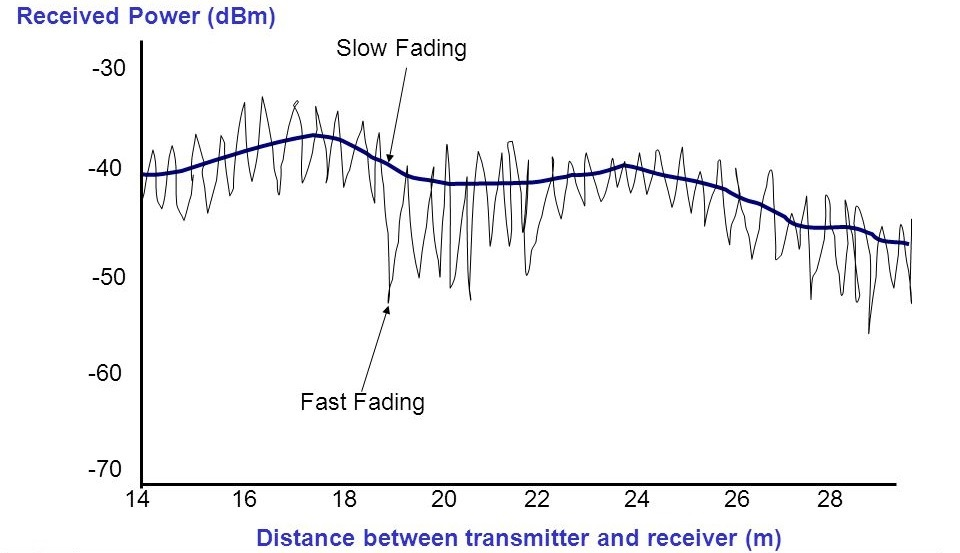
\includegraphics[scale=.5]{figuras/Slow-Fast-Fading.jpg}
	}{
		\Fonte{\citeonline{akkaya2019}.}
	}
\end{figure}

\section{Modelos de Propagação}
\label{sec:modelos-propagacao}

Para que se possa realizar um projeto de enlace de rádio confiável e com boa eficiência, são utilizados os chamados modelos de propagação. Os mesmos são desenvolvidos com base em medições empíricas que buscam alimentar com dados todo um processo matemático complexo capaz de representar a proliferação das ondas de rádio, predizer a perda de caminho ou a cobertura efetiva de um transmissor \cite{akpaida2018,najnudel2004}. Assim, é fácil concluir que, quanto mais informações for possível representar nestas equações, mais precisa será a caracterização do meio e seus efeitos \cite{akpaida2018}.

Modelos de propagação de rádio são empíricos por natureza. E como todos os modelos empíricos, os modelos de propagação de rádio não chamam a atenção para a conduta exata de uma conexão, mas sim para prever o comportamento que o \textit{link} pode mostrar sob as condições especificadas \cite{akpaida2018}.

Existem diversos modelos de propagação formulados por estudiosos e organizações voltadas para o ramo das comunicações sem fio. Cada modelo aplica-se a uma determinada situação específica, dependendo da característica física do local (região urbana ou região rural, por exemplo); frequência de operação do sistema de comunicação e o tipo de material da construção, fator este, crítico para as redes Wi-Fi.

\subsection{Modelo de propagação no espaço livre}
\label{sub:espaco-livre}

O modelo de propagação no espaço livre é usado para prever a intensidade do sinal recebido quando o transmissor e o receptor possuem um linha de visada, ou seja, um caminho livre entre eles \cite{rappaport2009}. Os sistemas de comunicação via satélite normalmente experimentam uma transmissão com caminho desobstruído.

O modelo de espaço livre, assim como a maioria dos modelos de propagação de radiofrequência, prevê que a potência recebida diminui em função da distância de separação transmissor-receptor (T-R) \cite{rappaport2009}. A potência no espaço livre recebida por uma antena receptora que está separada de uma antena transmissora, irradiando, por uma distância T-R é dada pela equação do espaço livre:

\begin{equation}
	\begin{aligned}
	\label{eq:friis}
		P_R = \dfrac{P_TG_TG_R}{L_P}
	\end{aligned}
\end{equation}

\noindent onde $P_T$ é a potência transmitida, $P_R$ é a potência recebida, $G_T$ é o ganho da antena transmissora, $G_R$ é o ganho da antena receptora e $L_P$ é a perda do percurso entre T-R. Tanto a dedução matemática do ganho da antena ($G$) quanto a da perda do percurso ($L_P$) pode ser encontrada com detalhes em \citeonline{haykin2008}.

A Eq. \eqref{eq:friis} é conhecida como equação de Friis. É possível simplificá-la em função do ganho em decibel (dB) \cite{haykin2008}:
\begin{equation}
	\begin{aligned}
	\label{eq:friis-decibel}
		P_R(dB) = P_T(dB) + G_T(dB) + G_R(dB) - L_P(dB)
	\end{aligned}
\end{equation}

\noindent onde $X(dB) = 10\log_{10} (X)$. A equação de Friis é a equação fundamental para o planejamento do enlace de rádio, pois relaciona as potências transmitida e recebida, considerando as condições da transmissão \cite{haykin2008}. Ela fornece os requisitos essenciais para que o nível de potência requerida pelo receptor seja suficiente para ele detectar as informações que lhe foram transmitidas com confiabilidade \cite{haykin2008}.

\subsection{Modelo de dois raios}
\label{sub:modelo-2-raios}

A equação do espaço livre (Eq. \eqref{eq:friis}) considera que sempre existe uma linha de visada direta entre transmissor e receptor, não considera, entretanto, o efeito da superfície terrestre na comunicação. Esse fato raramente acontece com transmissões em solo, o que torna o modelo de espaço livre impreciso na grande maioria dos casos \cite{rappaport2009}.

O modelo de reflexão no solo, baseado na ótica geométrica, considera o caminho direto e um caminho de propagação refletido no solo entre o transmissor e o receptor, como ilustra a \autoref{fig:2raios} \cite{rappaport2009}.

\begin{figure}[H]
	\centering
	\Caption{\label{fig:2raios}Modelo de reflexão no solo com dois raios.}	
	\UECEfig{}{
		%\fbox{\begin{varwidth}{\dimexpr\textwidth-2\fboxsep-2\fboxrule\relax}
		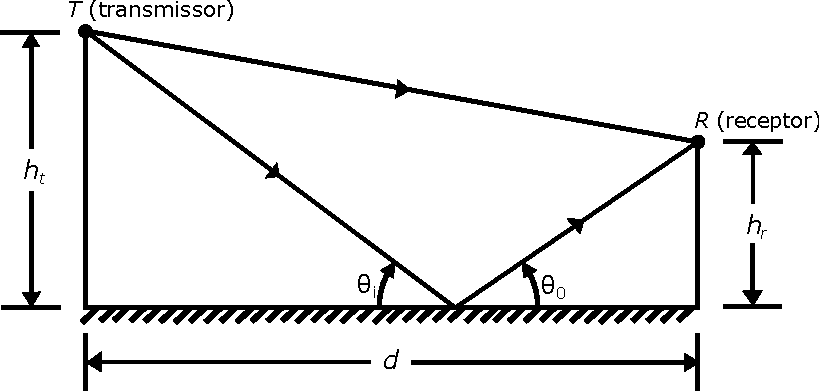
\includegraphics[scale=.4]{figuras/modelo2raios.pdf}
		%\end{varwidth}}
	}{
		\Fonte{Adaptado de \citeonline[p. ~80]{rappaport2009}}
	}
\end{figure}

A potência recebida a uma distância $d$ do transmissor para o modelo de dois raios pode ser expressa como \cite{rappaport2009}:
\begin{equation}
	\begin{aligned}
	\label{eq:2-raios}
		P_R = P_TG_TG_R\dfrac{h^2_Th^2_R}{d^4}
	\end{aligned}
\end{equation}

\noindent onde $h_T$ é a altura do transmissor e $h_R$ é a altura do receptor. Todo o desenvolvimento algébrico até chegar a Eq. \eqref{eq:2-raios} pode ser encontrada em \citeonline{rappaport2009} ou \citeonline{haykin2008}.

\subsection{Modelo log-distância (log simplificado)}
\label{sub:log-distancia}

Os modelos de propagação baseados em medições em campo indicam que que a potência média do sinal recebida cai logaritmicamente com a distância, seja em enlaces de rádio para ambientes fechados (\textit{indoor}) ou abertos (\textit{outdoor}) \cite{rappaport2009}. A perda de percurso média para a uma separação T-R qualquer é obtida em função da distância usando um expoente de perda de caminho, $n$, dada por
\begin{equation}
	\begin{aligned}
	\label{eq:log-distancia}
		PL(d) \propto \left(\dfrac{d}{d_0}\right)^n
	\end{aligned}
\end{equation}

\noindent ou

\begin{equation}
	\begin{aligned}
	\label{eq:log-distancia-2}
		PL(dB) = PL(d_0) + 10n\log_{10}\left(\dfrac{d}{d_0}\right)^n
	\end{aligned}
\end{equation}

\noindent onde $PL$ é a perda média do percurso, $n$ é o expoente de perda de caminho (indica a velocidade com a qual essa perda aumenta com relação a distância), $d_0$ é a distância de referência próxima que é determinada pelas medições perto do transmissor, e $d$ é a distância de separação T-R. O valor de $n$ é calculado usando-se a equação de Friis (modelo de espaço livre) ou por medições de campo à distância $d_0$. A Tabela 1 lista os expoentes típicos de perda de percurso em diversos ambientes.

\begin{table}[H]
	\Caption{\label{tab:tabela-perda-de-percusso}Expoentes de perda de percurso ($n$) para diferentes ambientes.}%
	\IBGEtab{}{%
		\begin{tabular}{lc}
			\toprule
			\multicolumn{1}{c}{Ambiente} & \multicolumn{1}{c}{Expoente de perda de percurso ($n$)} \\
			\toprule %\midrule
			Espaço livre & 2 \\
			
			Rádio-celular em área urbana & 2,7 a 3,5 \\
			
			Rádio-celular urbano sombreado & 3 a 5 \\
			
			Na linha de visão do prédio & 1,6 a 1,8 \\
			
			Obstruído no prédio & 4 a 6 \\
			
			Obstruído em prédio & 2 a 3 \\
			\bottomrule
		\end{tabular}%
	}{%
		\Fonte{\citeonline[p.~91]{rappaport2009}.}%
		%\citeonline[p. ~465]{lott2001ieee}; \apudonline[p.~73]{lott2001ieee}{geier2002}
	}%
\end{table}

\subsection{Modelo de Okumura--Hata}
\label{sub:okumura-hata}

O modelo de Okumura-Hata baseia-se em medições puramente empíricas voltadas especificamente para a predição de sinal de redes celulares para diferentes ambientes. A melhor aplicação do modelo de Okumura-Hata acontece na faixa de frequência existente entre 150 MHz e 1 GHz, podendo ser estendido até 1,5 GHz \cite{haykin2008,rappaport2009}. 

Os dados originais foram medidos por Okumura (entre outros) em diversos locais do Japão. Algum tempo depois, Hata forneceu a equação para predição da perda de propagação em área urbana, juntamente com outras equações de correção para aplicações em área suburbana e aberta.

As perdas do percurso, em dB, para esses três tipos de meios, respectivamente, são dadas pelas equações
\begin{equation}
\begin{split}
	\label{eq:okumura-hata}
		L_P & = A + B\log_{10}r \\
		L_P & = A + B\log_{10}r - C \\
		L_P & = A + B\log_{10}r - D
\end{split}
\end{equation}

\noindent onde $r$ é o alcance em quilômetros, os parâmetros $A$, $B$, $C$ e $D$\footnote[2]{As equações que permitem determinar os valores de $A$, $B$, $C$ e $D$ fogem ao escopo deste trabalho e, por isso, podem ser encontrados na literatura em \citeonline{haykin2008}.} dependem da frequência de operação ($f_c$), da altura da estação transmissora ($h_T$) e da altura da estação receptora ($h_R$).

\subsection{Modelo Multi--Wall--and--Floor}
\label{sub:modelo-MWF}

O modelo \emph{Multi-Wall-and-Floor} (MWF) leva em consideração a perda decrescente de penetração de paredes/pisos da mesma categoria, à medida que o número de paredes/pisos atravessados aumenta, isto é, defende que a relação entre as  perdas não segue uma linearidade lógica \cite{lott2001ieee}. Por exemplo, dada uma perda de penetração de 2 dB em uma parede de concreto, essa mesma onda, ao penetrar em outra parede de mesma característica, não sofrerá uma atenuação de 2 dB como ocorrido no primeiro obstáculo.

O modelo MWF, proposto por \citeonline{lott2001ieee}, é voltado especialmente para a análise dos efeitos da propagação em ambientes \textit{indoor}, pois esses locais concentram grande variedade de divisórias construídas com diferentes materiais. A perda sofrida por uma onda de rádio ao atravessar múltiplas paredes/pisos, $L_{P}$, pode ser dada pela seguinte equação:
\begin{equation}
	\begin{aligned}
	\label{eq:mwf}
		L_{P} = L_0 + 10n\log_{10}(d) + \sum_{i=1}^{I} \sum_{k=1}^{K_{wi}} L_{wik} + \sum_{j=1}^{J} \sum_{k=1}^{K_{fj}} L_{fjk}
	\end{aligned}
\end{equation}

\noindent onde $L_0$ é a perda de trajetória a uma distância de 1m, $n$ é o fator de perda do percurso, $d$ é a distância entre o transmissor e o receptor, $L_{wik}$ é a atenuação devido ao tipo de parede $i$ e à $k$-ésima parede atravessada, $L_{fjk}$ é a atenuação devida ao tipo de piso $j$ e ao $k$-ésimo piso atravessado, $I$ é o número de tipos de parede, $J$ é o número de tipos de piso, $K_{wi}$ é o número de paredes atravessadas do tipo $i$ e $K_{fj}$ é o número de paredes atravessadas do tipo $j$. 

O valor da perda de penetração varia de acordo com o tipo de material ao qual o obstáculo foi construído. A \autoref{tab:tabela-mwf} lista alguns valores de perda de penetração para diversos tipos de material para medições feitas na faixa de frequência de 5.8 GHz.

\begin{table}[H]
	\Caption{\label{tab:tabela-mwf}Valores de perda de penetração da parede para o modelo MWF para 5.8 GHz.}%
	\IBGEtab{}{%
		\begin{tabular}{lcc}
			\toprule
			\multicolumn{1}{c}{Material da parede} & \multicolumn{1}{c}{Espessura} & \multicolumn{1}{c}{$k=1$} \\
			\toprule %\midrule
			Madeira compensada & 0.4 cm & $L_{w1I} = 0.9\ dB$ \\
			
			Parede de gesso (rebocada com 1mm de gesso) & 13.5 cm & $L_{w2I} = 3.0\ dB$ \\
			
			Aglomerado de madeira & 1.5 cm & $L_{w3I} = 1.0\ dB$ \\
			
			Vidro plano &  & $L_{w4I} = 2.5\ dB$ \\
			
			Janela de vidro duplo (com uma camada de ar de 12mm) & 2.0 cm & $L_{w5I} = 12\ dB$ \\
			
			Parede de bloco de concreto armado & 30.2 cm & $L_{w6I} = 10\ dB$ \\
			\bottomrule
		\end{tabular}%
	}{%
		\Fonte{Adaptado de \apudonline[p. ~467]{lott2001ieee}{ERC1999}.}%
	}
\end{table}

	\chapter{Redes Wi-Fi}
\label{cap:redes-wifi}

\section{Introdução}
\label{sec:introducao}

Ao longo dos anos, a evolução  dos sistemas e serviços de telecomunicações criou uma necessidade para seus usuários de estarem conectados ``todo tempo'' e ``em qualquer lugar'', isto é, esses usuários desejam estar permanentemente \textit{online}. Para esses usuários, os meios guiados (par trançado, cabo coaxial e fibra óptica) não têm a menor utilidade, pois uma característica essencial para cumprimento destas necessidades é a mobilidade.

No período em que as LANs cabeadas dominavam a infraestrutura de rede de computadores, somente era possível conectar computadores à Internet e entre si por meio de cabos padrão Ethernet. Este tipo de conexão é bastante popular, mas conta com algumas limitações, por exemplo: só se pode movimentar o computador até o limite de alcance do cabo; ambientes com um grande número computadores podem exigir adaptações na estrutura do prédio para a passagem dos fios; em uma residência, pode ser necessário realizar perfurações na parede para que os cabos alcancem outros cômodos; a manipulação constante ou incorreta pode fazer com que o conector do cabo de rede se danifique \cite{alecrim2008site}.

Usuários móveis precisam transferir dados para seus dispositivos sem depender da infraestrutura de comunicação cabeada tradicional \cite{tanenbaum2011}. A resposta para esses usuários está na comunicação sem fios. Dentro das comunicações \textit{wireless}, as LANs sem fio oferecem uma alternativa bastante interessante como meio de acesso à Internet.

As LANs sem fio são muito populares atualmente, especialmente nas residências, escritórios, instituições acadêmicas e outros lugares onde a instalação de cabos é muito trabalhosa ou inviável física e/ou financeiramente. Embora muitas tecnologias e padrões para LANs sem fio tenham sido desenvolvidos na década de 1990, uma classe particular de padrões surgiu claramente como a vencedora: a LAN sem fio IEEE 802.11, também conhecida como Wi-Fi \cite{kurose2013}.

Wi-Fi, acrônimo de \textit{Wireless Fidelity}\footnote{Apesar de que a Wi-Fi Alliance nunca ter afirmado tal conclusão.} é o termo comumente usado para tecnologia que é padronizado pelo Instituto de Engenheiros Elétricos e Eletrônicos (IEEE, do inglês, \textit{Institute of Eletrical and Eletronics Engineers}) sob seus 802 padrões de redes locais. Estritamente falando, ``Wi-Fi'' é o nome da marca comercial dado a produtos que são certificados para serem interoperáveis pela Wi-Fi Alliance\footnote{https://www.wi-fi.org/}, que é uma associação comercial que promove o Wi-Fi e realiza as certificações de equipamentos \cite{gorshe2014ieee}.

O padrão Wi-Fi opera nas faixas de 2,4 GHz e 5 GHz, dentro das faixas livres ISM. De qualquer forma, a desregulamentação do espectro da banda ISM estimulou décadas de inovação e tem sido o principal facilitador do acesso sem fio onipresente atualmente \cite{gorshe2014ieee}.

Outro motivo para a proliferação de implementações Wi-Fi é a facilidade de configuração e compatibilidade com as redes Ethernet com fio que precederam o Wi-Fi \cite{gorshe2014ieee}. No ambiente doméstico, a instalação de redes Wi-Fi tem sido relativamente livre de problemas. Mesmo para aqueles que não são tecnicamente experientes, uma instalação profissional não é cara, e geralmente pode ser fornecida pelo provedor de serviços de Internet local.

\section{Elementos de uma Rede Wi-Fi}
\label{elementos-rede-wifi}

Assim como telefones celulares, televisões e rádios, uma rede Wi-Fi usa ondas de rádio que se propagam ao redor do ponto de acesso para estabelecer a comunicação entre os terminais conectados a ele.

Para que os dados possam ser enviados, o adaptador de rede do cliente os converte em sinal de rádio e os transmite através de uma antena. O ponto de acesso recebe o sinal e o decodifica para então enviá-los para a Internet usando uma conexão Ethernet física com fio padrão \cite{brain2001}.

O processo inverso também funciona, com a estação-base recebendo dados da Internet, convertendo-os em um sinal de rádio e enviando-os ao adaptador sem fio do dispositivo de destino \cite{brain2001}.
Para que uma rede Wi-Fi exista e funcione como descrito anteriormente são necessários alguns componentes que desempenham funções fundamentais, tais como:

\begin{compactitem}
	\item Hospedeiros sem fio: são os dispositivos finais que utilizam os serviços providos pelo ponto de acesso (definido mais adiante). Um hospedeiro sem fio pode ser um \textit{notebook}, um \textit{tablet}, um \textit{smartphone} ou um computador de mesa compatível \cite{kurose2013};
	\item Estação-base (ou ponto de acesso): as estações-base são partes fundamentais da infraestrutura de uma rede sem fio, elas possuem a responsabilidade de coordenar as transmissões dos hospedeiros a elas associadas \cite{kurose2013};
	\item Enlaces sem fio: são responsáveis pela comunicação dos hospedeiros com a ponto de acesso por meio de um enlace de rádio, podem possuir taxas, distância e frequência de transmissão diferentes \cite{kurose2013};
	\item Infraestrutura de rede: cada estação-base está conectada a uma rede maior. Além disso, toda a comunicação é feita entre a estação-base e um hospedeiro sem fio através de um único salto sem fio, ou seja, sem nós intermediários \cite{kurose2013}.
\end{compactitem}

A disposição dos elementos descritos anteriormente pode ser vista na \autoref{fig:elementos-rede}.

\begin{figure}[H]
	\centering
	\Caption{\label{fig:elementos-rede}Elementos de uma rede Wi-Fi padrão.}	
	\UECEfig{}{
		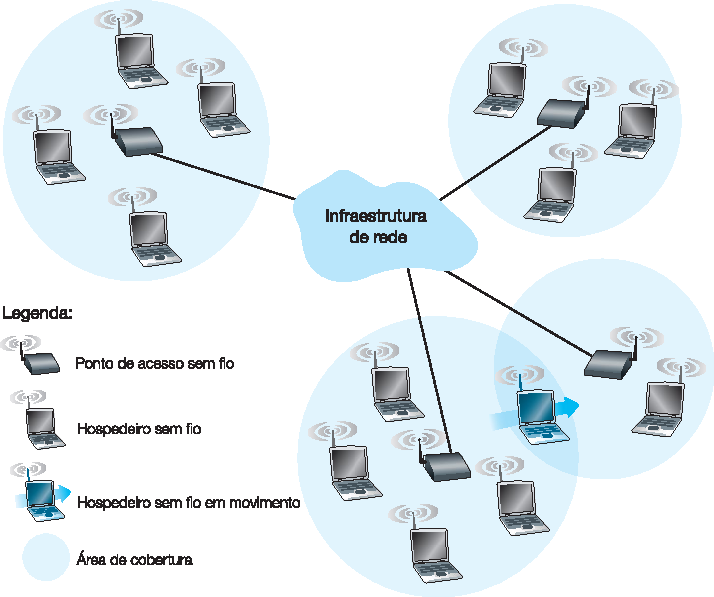
\includegraphics[scale=.77]{figuras/elementos_rede_wireless.pdf}
	}{
		\Fonte{\citeonline[p. ~383]{kurose2013}.}
	}	
\end{figure}

\section{Topologias de LANs sem Fio}
\label{topologias-lans-sem-fio}

As LANs sem fio podem ser estruturadas para operar em dois modos: modo de infraestrutura e modo \textit{ad hoc}.

No modo de infraestrutura, mostrado na \autoref{fig:topologias}(a), cada cliente está associado a um ponto de acesso, que, por sua vez, está conectado a outra rede, geralmente à Internet. O cliente transmite e recebe seus pacotes por meio do ponto de acesso \cite{tanenbaum2011}. Essa topologia é a mais comumente usada, e não é diferente da topologia de uma rede celular.

O outro modo, mostrado na \autoref{fig:topologias}(b), é um exemplo de rede \textit{ad hoc}. Esse modo é um conjunto de terminais móveis que estão interligados de modo que possam enviar dados diretamente uns aos outros. Não existe ponto de acesso nessa configuração, portanto os próprios dispositivos são responsáveis pelo gerenciamento dos recursos da rede. Porém, como o acesso à Internet é a principal aplicação para redes sem fio, as redes \textit{ad hoc} não são muito populares \cite{tanenbaum2011}.

\begin{figure}[H]
	\centering
	\Caption{\label{fig:topologias}Topologias de redes sem fio. (a) Modo de infraestrutura. (b) Modo \textit{ad hoc}.}	
	\UECEfig{}{
		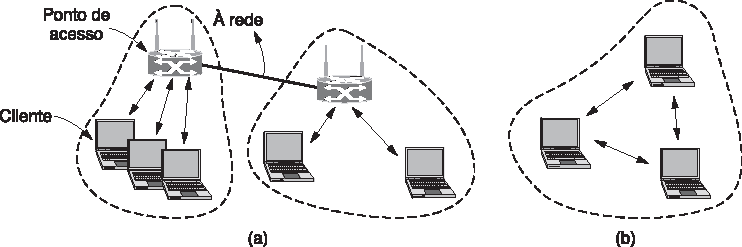
\includegraphics[scale=.9]{figuras/arquiteturas_802-11_tanenbaum.pdf}
	}{
		\Fonte{\citeonline[p. ~188]{tanenbaum2011}.}
	}	
\end{figure}

\section{Visão geral do sistema Wi-Fi}
\label{sistema-wifi}

Um sistema de LAN sem fio Wi-Fi geralmente consiste em dois tipos de nós: clientes e pontos de acesso. O ponto de acesso (\autoref{fig:ap}), também chamado de roteador sem fio é o ponto central de qualquer rede sem fio. O ponto de acesso conecta todos os equipamentos sem fio à rede tradicional cabeada, onde está a conexão com a Internet.

\begin{figure}[H]
	\centering
	\Caption{\label{fig:ap}Ponto de acesso da fabricante 3Com.}	
	\UECEfig{}{
		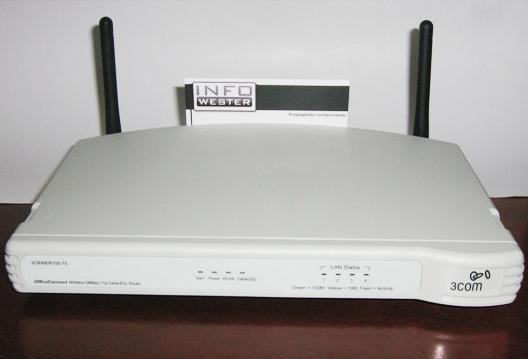
\includegraphics[scale=.62]{figuras/routerwf.jpg}
	}{
		\Fonte{\citeonline{alecrim2008site}.}
	}	
\end{figure}

Os clientes da rede sem fio são os computadores de mesa, \textit{notebooks}, agendas eletrônicas (PDA, do inglês, \textit{Personal Digital Assistant}), \textit{smartphones} e até consoles de videogame (\autoref{fig:clientes}). Para conectarem-se a uma rede sem fio, os equipamentos precisam ter uma interface Wi-Fi. Atualmente, a maioria dos clientes já possui uma placa Wi-Fi integrada de fábrica.

\begin{figure}[H]
	\centering
	\Caption{\label{fig:clientes}Exemplos de clientes sem fio.}	
	\UECEfig{}{
		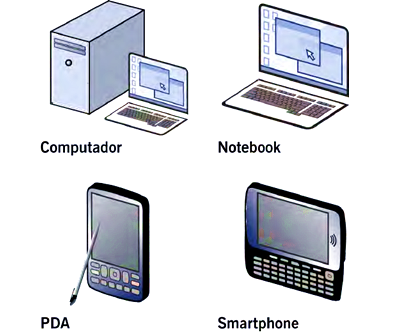
\includegraphics[scale=.75]{figuras/clientes.png}
	}{
		\Fonte{\citeonline[p. ~8]{fluminense2010}.}
	}	
\end{figure}

\section{Arquitetura da LAN sem Fio 802.11}
\label{arquitetura-802-11}

A \autoref{fig:arquitetura} ilustra os principais elementos da arquitetura de uma LAN sem fio 802.11. O bloco de construção fundamental da arquitetura 802.11 é o Conjunto Básico de Serviço (BSS, do inglês, \textit{Basic Service Set}). Um BSS contém uma ou mais estações sem fio e um ponto de acesso e possui a função de controlar quando cada cliente móvel pode transmitir. O Sistema de Distribuição (DS, do inglês, \textit{Distribution System}) é o local da topologia onde os pontos de acesso se interconectam numa rede cabeada, podendo ser numa rede padrão Ethernet ou num \textit{backbone}. O Ponto de Serviço Estendido (ESS, do inglês, \textit{Extended Service Set}) é o ponto ou um grupo de pontos básicos de serviço interconectados por um sistema de distribuição \cite{moraes2010}.

\begin{figure}[H]
	\centering
	\Caption{\label{fig:arquitetura}Arquitetura típica de uma LAN IEEE 802.11.}	
	\UECEfig{}{
		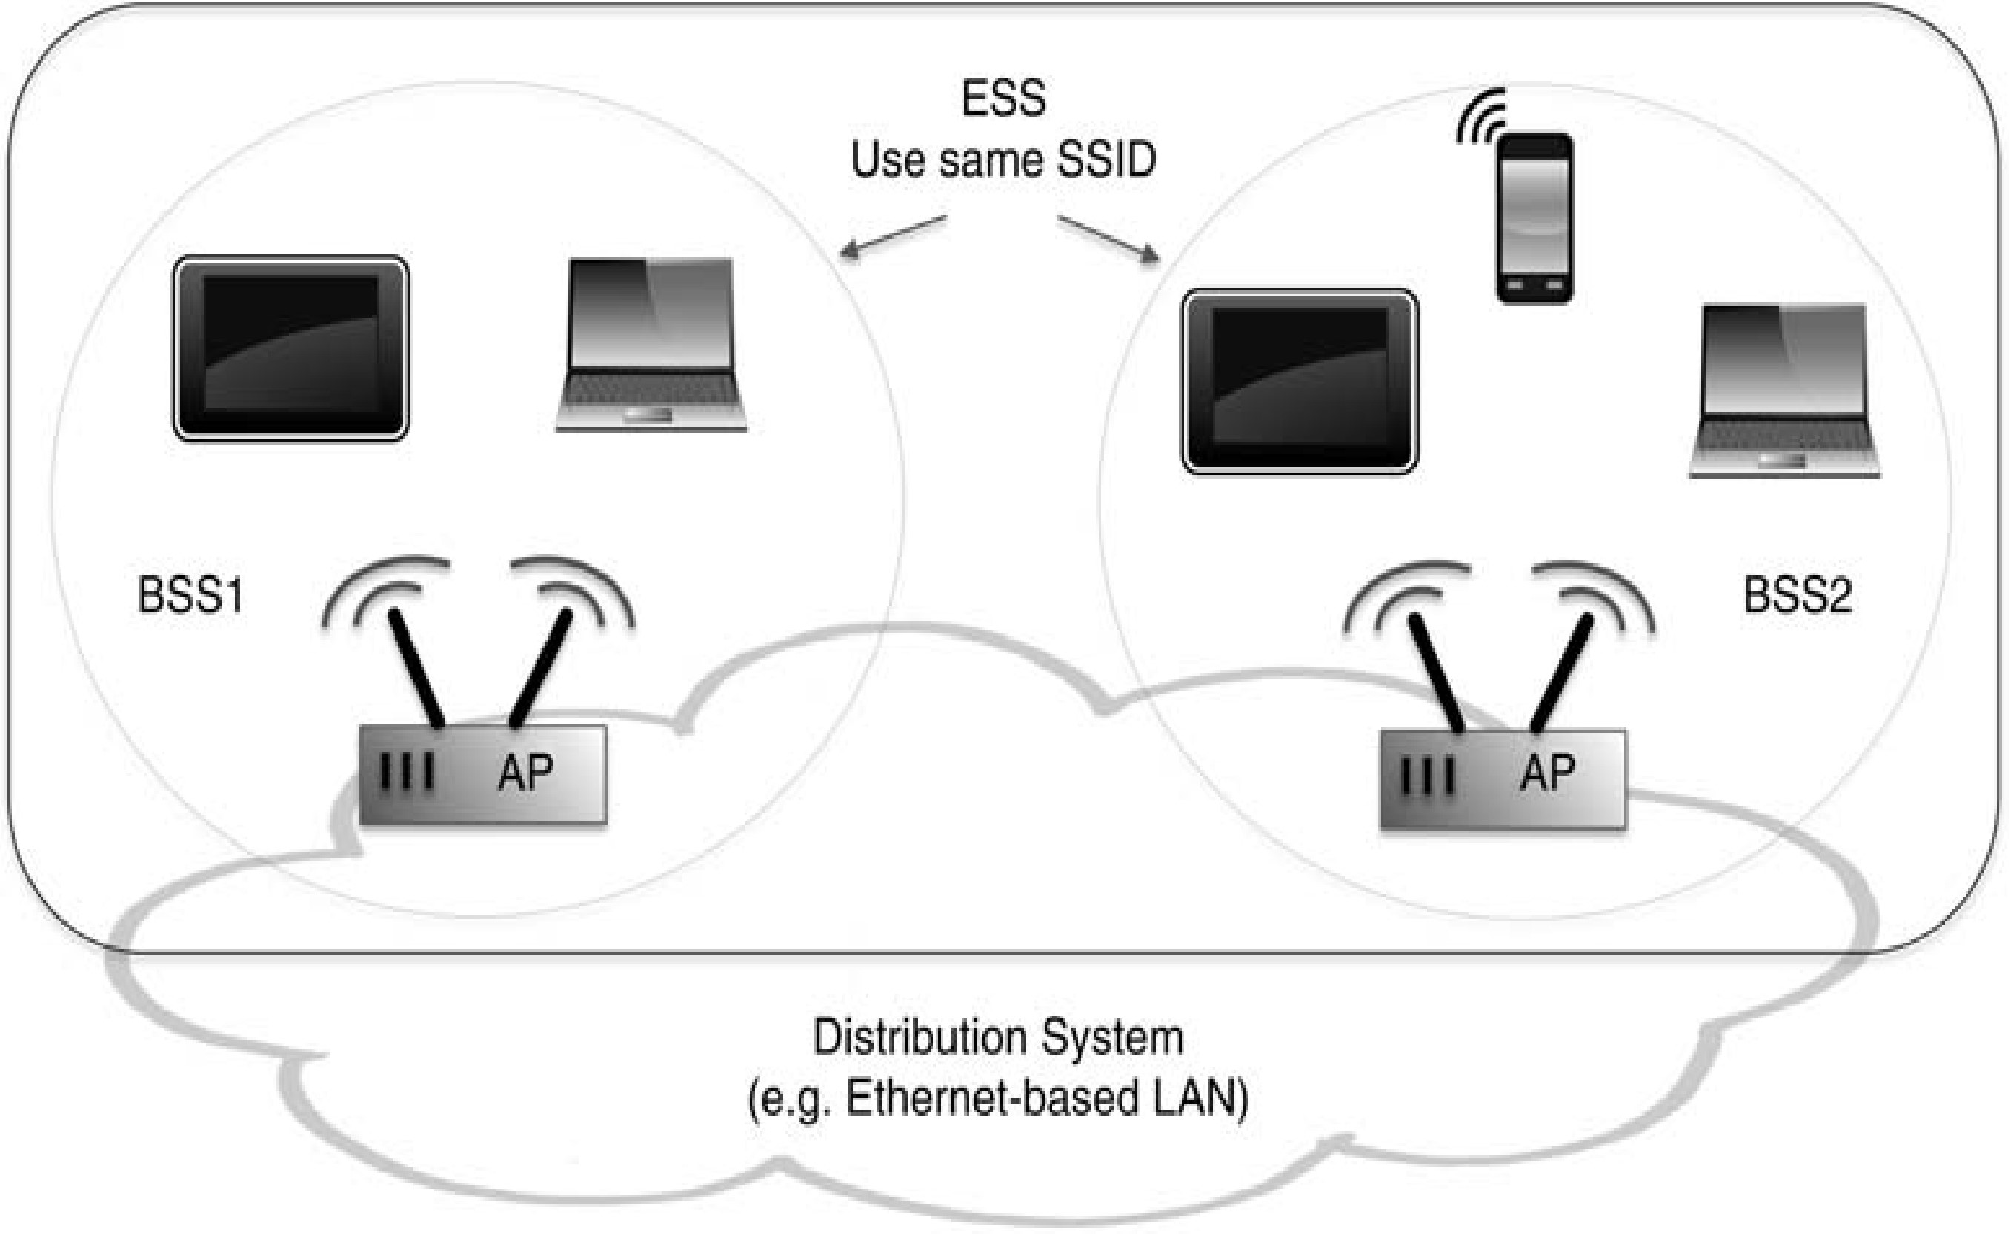
\includegraphics[scale=.33]{figuras/arquiteturas_802-11_01.pdf}
	}{
		\Fonte{\citeonline[p. ~308]{gorshe2014ieee}.}
	}	
\end{figure}

Outro ponto importante na arquitetura 802.11 consiste no fato de a rede permitir a mudança automática e transparente para o usuário quando este sai de sua célula (BSS) e vai para outra célula vizinha, processo este conhecido como \textit{roaming}. Cada célula contém o seu ponto de acesso e por esse motivo o \textit{roaming} multicanal oferece maior abrangência e mobilidade ao sistema (MORAES, 2014).

\section{Padrão IEEE 802.11}
\label{padrao-ieee-802-11}

Desde a introdução das redes sem fio como meio de acesso à Internet, o sucesso das mesmas só cresceu, com isso várias empresas procuram formas de padronizar essa tecnologia. O problema é que cada empresa criou seu próprio padrão de rede, o que dificultava a compatibilidade entre equipamentos e protocolos.
Entretanto, para que os equipamentos pudessem se comunicar entre si, deveriam usar os mesmos padrões de comunicação. Com o objetivo de garantir a interoperabilidade dos diversos tipos de equipamentos e fabricantes existentes, os membros do IEEE criaram, em 1997, após sete anos de pesquisa e desenvolvimento, o padrão IEEE 802.11, o primeiro a ser desenvolvido por uma instituição independente, o que impulsionou a sua grande aceitação entre as empresas fabricantes de equipamentos \cite{fluminense2010}.

À medida que a tecnologia de redes sem fio evoluiu, o padrão IEEE 802.11 foi expandido de forma a melhorar aspectos da rede, como a taxa de transmissão e a segurança. Estas melhorias foram incorporadas sob a forma de ``emendas'', designadas por letras acrescentadas ao nome do padrão, como, por exemplo, IEEE 802.11a \cite{fluminense2010}. A seguir, algumas das principais ``emendas'' são explicadas com algum detalhe, de acordo com o ano de surgimento.

\subsection{IEEE 802.11b}
\label{802-11b}

O padrão 802.11b foi o primeiro padrão IEEE 802.11 aprovado a se popularizar em setembro de 1999. Ele opera na faixa entre 2,4 e 2,4835 GHz e tem a possibilidade de estabelecer conexões nas seguintes velocidades de transmissão: 1 Mbps, 2 Mbps, 5.5 Mbps e 11 Mbps \cite{moraes2010,fluminense2010}.

\subsection{IEEE 802.11a}
\label{802-11a}

O padrão 802.11a foi lançado no mesmo ano que o 802.11b e, apesar de oferecer taxas mais altas, não alcançou a mesma popularidade. As taxas adicionais oferecidas pela emenda “a” são: 6 Mbps, 9 Mbps, 12 Mbps, 18 Mbps, 24 Mbps, 36 Mbps, 48 Mbps e 54 Mbps.

As frequências utilizadas por este padrão estão entre 5,725 e 5,875 GHz. Nesta faixa de frequência mais alta, o sinal é mais suscetível a perdas de propagação, diminuindo seu alcance em comparação com a faixa utilizada pelo IEEE 802.11b. Em contrapartida, o uso desta frequência pode ser atraente por estar menos sujeita a interferência de outras fontes. Não existe compatibilidade entre o 802.11a e o 802.11b, pois eles operam em duas faixas de frequência distintas \cite{moraes2010,fluminense2010}.

\subsection{IEEE 802.11g}
\label{802-11g}

O padrão 802.11g, lançado em 2003, pode ser considerado o sucessor do padrão 802.11b, pois opera na mesma faixa de frequência de 2,4 GHz. Dispositivos que implementam o 802.11g costumam ser retrocompatíveis, isto é, implementam também o 802.11b, sendo muitas vezes especificados como dispositivos 802.11b/g. Sua principal vantagem é a possibilidade de operar com taxas de transmissão de até 54 Mbps, como o IEEE 802.11a, e ao mesmo tempo ter o alcance do IEEE 802.11b \cite{moraes2010,fluminense2010}.

\subsection{IEEE 802.11n}
\label{802-11n}

O desenvolvimento do padrão 802.11n foi iniciado em 2004 e publicado em 2009. Este padrão pode operar nas faixas de 2,4 GHz e 5 GHz, o que o torna compatível com os padrões anteriores. Sua principal característica é o aumento considerável das taxas de transferência de dados através da combinação de múltiplas vias de transmissão (MIMO, do inglês, \textit{Multiple-Input and Multiple-Output}). O padrão 802.11n pode operar com taxas de transmissão de dados de até 600 Mbps em um canal de 40 MHz \cite{moraes2010}.

\subsection{IEEE 802.11ac}
\label{802-11ac}

O padrão IEEE 802.11ac foi desenvolvido entre 2011 e 2013 e publicado em dezembro de 2013. Pode ser considerado como o sucessor, em termos de taxa de transmissão, do IEEE 802.11n \cite{alecrim2008site}.
A principal vantagem do 802.11ac está em sua velocidade, estimada em até 433 Mbps no modo mais simples. Mas, teoricamente, é possível fazer a rede superar os 6 Gbps em uma configuração que utiliza múltiplas antenas transmissoras (no máximo, oito antenas podem ser utilizadas). Pelo fato dos equipamentos comumente saírem de fábrica com três antenas, a taxa máxima de transmissão é de aproximadamente de 1,3 Gbps \cite{alecrim2008site}.

O 802.11ac trabalha na frequência de 5 GHz, sendo que, dentro desta faixa, cada canal pode ter, por padrão, largura de 80 MHz ou 160 MHz como opcional. Além disso, o 802.11ac possui técnicas de modulação avançadas. Precisamente, o padrão trabalha com a técnica MU-MIMO (do inglês, \textit{Multi-User} MIMO), que permite que sejam transferidos e recebidos dados simultaneamente para todos os terminais, o que resulta em uma melhoria nas velocidades de transferência na mesma frequência de operação \cite{alecrim2008site}.

\subsection{IEEE 802.11ax}
\label{802-11ax}

O padrão 802.11ax, chamado Wi-Fi 6, um nome mais simples e comercial atribuído pela Wi-Fi Alliance, é o sucessor do 802.11ac. Até momento deste trabalho o Wi-Fi 6 encontra-se em processo de desenvolvimento. Entretanto, já existe fabricantes trabalhando em novos equipamentos compatíveis com o novo padrão de rede sem fio \cite{plaza2018site}.

Com o IEEE 802.11ax a previsão é que os equipamentos consigam operar com a velocidade máxima de 14 Gbps, enquanto na prática a transmissão estará próxima dos 11 Gbps. Diferentemente do 802.11ac que opera apenas na banda de 5 GHz, o Wi-Fi 6 é \textit{dual band} (opera em 2,4 GHz e 5 GHz). Outras promessas são um consumo de energia menor para os dispositivos conectados e uma maior capacidade em manter um bom alcance mesmo com a presença de barreiras, como paredes, que acabam atrapalhando a propagação do sinal pelo ambiente \cite{plaza2018site}.

A visão resumida dos padrões IEEE 802.11 apresentados anteriormente é mostrada na \autoref{tab:resumo-ieee-802-11}.

\begin{table}[H]
	\Caption{\label{tab:resumo-ieee-802-11}Resumo dos padrões IEEE 802.11.}%
	\IBGEtab{}{%
		\begin{tabular}{lccc}
			\toprule
			\multicolumn{1}{c}{Padrão} & \multicolumn{1}{c}{Ano} &  \multicolumn{1}{c}{Banda de Frequência} &  \multicolumn{1}{c}{\textit{Throughput} Máximo (Proposto)} \\
			\toprule %\midrule
			IEEE 802.11b & 1999 & 2.4 GHZ & 11 Mbps \\
			
			IEEE 802.11a & 1999 & 2.4 GHz & 54 Mbps \\
			
			IEEE 802.11g & 2003 & 5 GHz & 54 Mbps \\
			
			IEEE 802.11n & 2009 & 2.4 GHz/5 GHz & 600 Mbps \\
			
			IEEE 802.11ac & 2013 & 5 GHz & 6 Gbps \\
			
			IEEE 802.11ax & Em desenvolvimento & 2.4 GHz/5 GHz & 14 Gbps \\
			\bottomrule
		\end{tabular}%
	}{%
		\Fonte{Adaptado de \citeonline{kar2018ieee}.}%
		%\citeonline[p. ~465]{lott2001ieee}; \apudonline[p.~73]{lott2001ieee}{geier2002}
		\Nota{{\textit{Throughput}, em português, significa taxa de transferência.}}
	}%
\end{table}

\section{Planejamento/Avaliação de Redes Wi-Fi}
\label{sec:alanejamento-avaliação-de-redes-wifi}

Caso surja a necessidade de se planejar a conexão de dispositivos em escritório, residência ou \textit{campus} em uma rede, a implantação da tecnologia Wi-Fi é a solução mais fácil e rápida. A implantação adequada dos componentes básicos (pontos de acesso, cabos e conectores) e a sintonia entre eles é o principal requisito para uma comunicação eficiente e rápida entre os terminais \cite{kar2018ieee}. Para obter um desempenho otimizado de uma LAN sem fio Wi-Fi, é essencial realizar o \textit{site survey} e o planejamento de radiofrequência antes da implantação.

Porém, é importante salientar que uma rede sem fio jamais chega ao mesmo nível de performance da rede cabeada tradicional \cite{moraes2010}. Consideremos também que o meio não guiado e a frequência são compartilhados: quanto mais estações conectadas, menor o desempenho final da rede.

\section{Site Survey}
\label{sec:site-survey}

Um procedimento muito importante para o projeto de uma rede sem fio é a utilização de uma metodologia chamada \textit{site survey} (em português, pesquisa do local). Essa metodologia consiste na inspeção técnica minuciosa do local onde será instalada a nova rede, na avaliação dos resultados obtidos da infraestrutura existente ou na identificação e solução dos problemas de um sistema já em funcionamento \cite{pinheiro2004site}.

O \textit{site survey} é uma ferramenta indispensável para detectar e ultrapassar problemas de performance após a implantação de uma nova infraestrutura ou ampliação da rede existente. Durante a inspeção do local, devem ser levantados dados técnicos das condições arquitetônicas do local, que inclui verificar a existência ou não de obstáculos que possam dificultar a distribuição do cabeamento, o posicionamento de equipamentos, a segurança do sistema, etc. \cite{moraes2010,pinheiro2004site}.

No caso específico das redes Wi-Fi, além das condições arquitetônicas do local, a inspeção deve contemplar a análise de possíveis fontes de interferência de radiofrequência, níveis e condições de propagação do sinal, área de cobertura (ou sem cobertura), servindo como fonte adicional de informação para o projeto de posicionamento dos pontos de acesso \cite{pinheiro2004site}. Em seguida, no planejamento de radiofrequência, finalizada a coleta de dados via \textit{site survey}, ajustes finais são feitos nos parâmetros de rede para obter um desempenho otimizado \cite{kar2018ieee}. A sequência completa de etapas do \textit{site survey} em redes \textit{wireless} está ilustrada pelo fluxograma da \autoref{fig:fluxograma-site-survey}. Para uma descrição mais detalhada de cada etapa do processo, consulte \citeonline{kar2018ieee}.

\begin{figure}[H]
	\centering
	\Caption{\label{fig:fluxograma-site-survey}Fluxograma para o processo completo do \textit{Site Survey}.}	
	\UECEfig{}{
		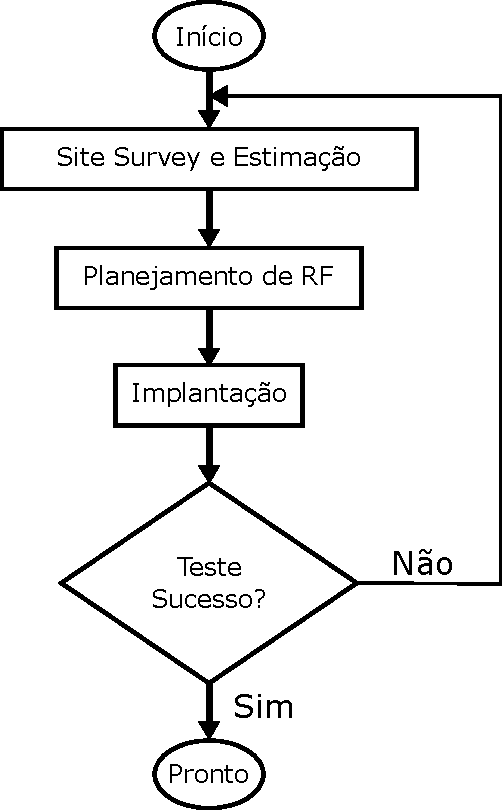
\includegraphics[scale=.7]{figuras/fluxograma_site_survey_01.pdf}
	}{
		\Fonte{Adaptado de \citeonline{kar2018ieee}.}
	}	
\end{figure}

O principal objetivo de um \textit{site survey} é assegurar que o número, localização e configuração dos pontos de acesso forneçam as funcionalidades requeridas e propiciem um desempenho compatível com a demanda exigida ou com o investimento definido no projeto \cite{pinheiro2004site}. Isso possibilita que todas as estações desfrutem de qualidade nas conexões, tendo total acesso aos serviços disponíveis na rede.

O problema encontrado com maior frequência em redes sem fio é a degradação do sinal devido aos múltiplos caminhos de propagação (multipercurso), causado por reflexões das ondas de rádio em objetos. Portanto, as antenas dos pontos de acesso devem estar dispostas longe de superfícies refletoras, a fim de diminuir as perdas causadas por esse fenômeno \cite{kar2018ieee}.

O processo de pesquisa do local pode ser executado manualmente ou usando um software dedicado. A pesquisa manual consiste essencialmente de uma avaliação baseada em \textit{hardware} posteriormente a implantação da rede, enquanto a pesquisa preditiva do local, além da pesquisa em si, inclui o planejamento baseado em simulação computacional \cite{kar2018ieee}.

É possível classificar o \textit{site survey} para redes sem fio em duas categorias dependendo do tipo de ambiente: (\textit{indoor}) ou (\textit{outdoor}).

\textit{Site survey indoor}: consiste em realizar a inspeção buscando interferências, localização e número de pontos de acesso. O equipamento utilizado é basicamente um \textit{notebook} provido de um software dedicado instalado e configurado. Esse tipo de inspeção fornece gráficos de intensidade de sinais (mapa de calor), o que torna o análise da cobertura mais precisa e clara. Em prédios, a inspeção pode ser executada em apenas um andar ou em múltiplos andares \apud[p.~73]{rodrigues2007}{geier2002}.

\textit{Site survey outdoor}: consiste em realizar a inspeção de redes \textit{wireless} em uma escala muito maior que a existente na modalidade \textit{indoor}. Além da localização e posição de pontos de acesso e das antenas de transmissão de grande porte, verifica-se a existência de linha de visada direta ou não com o fonte transmissora \cite{pinheiro2004site}. Essa modalidade de inspeção produz mapas de calor com maior complexidade de análise, devido às dimensões do terreno, da variabilidade do relevo e da grande quantidade de fontes de interferência \apud[p.~73]{rodrigues2007}{geier2002}.

\subsection{Softwares de Site Survey}
\label{subsec:softwares-site-survey}

Implantar uma rede Wi-Fi que cubra uma grande área e com um sinal forte não é uma tarefa fácil. Devido à interferência causada por outras redes Wi-Fi e à presença de grandes obstáculos tais como paredes e mobília, muitas redes Wi-Fi são castigadas por quedas frequentes da conexão, velocidades baixas, e a presença de zonas sem cobertura de sinal (áreas de sombra).

No entanto, é possível otimizar o desempenho de uma rede Wi-Fi com a ajuda de uma ferramenta de \textit{software} específica que gere, por exemplo, um mapa de calor, que consiste em um mapa da cobertura e força do sinal \textit{wireless} baseado na representação real do local de interesse. No mapa de calor é possível identificar, de acordo com a colorização dos setores, onde os nível de potência do sinal é mais forte ou mesmo inexiste, contribuindo para eventuais alterações na infraestrutura da rede.

\subsubsection{NetSpot}
\label{subsubsec:netspot}

Disponível para o sistema operacional MacOS e Windows, NetSpot é a ferramenta de \textit{software} de \textit{site survey} paga projetada para ser utilizada tanto por profissionais quanto por usuários domésticos. Dispõe de uma interface gráfica intuitiva, facilitando sua utilização.

Com o NetSpot é possível criar, na janela \textit{survey}, um mapa de calor a partir do \textit{upload} do arquivo que representa o local real (\autoref{fig:netspot}). Em seguida, basta o deslocamento de um local a outro para a coleta dos dados e aguardar a construção automática do gráfico com a intensidade do sinal de cada ponto. Além disso, o NetSpot possui a capacidade de analisador Wi-Fi, coletando informações detalhadas sobre as redes \textit{wireless} próximas, incluindo o seu nome (SSID, do inglês, \textit{Service Set Identifier}), o tipo de segurança que usam, em qual canal transmitem, e a potência do sinal, entre outras características \cite{Netspot2019}.

\begin{figure}[H]
	\centering
	\Caption{\label{fig:netspot}Tela de \textit{survey} do NetSpot.}	
	\UECEfig{}{
		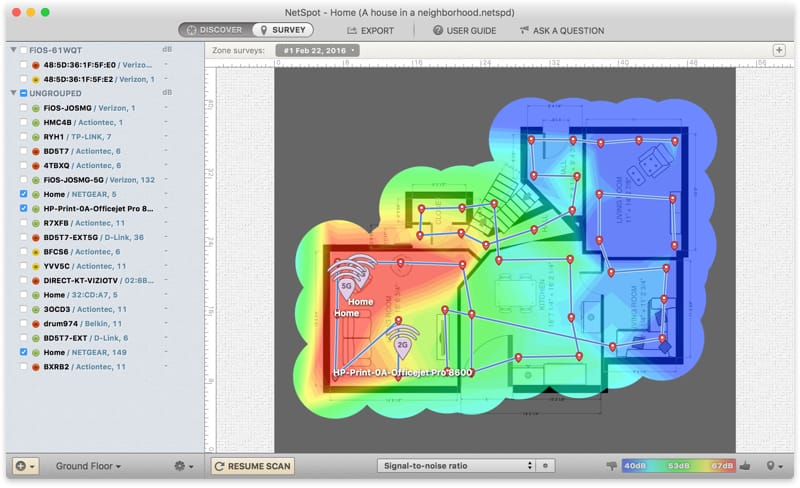
\includegraphics[scale=.48]{figuras/tela_netspot.jpg}
	}{
		\Fonte{\citeonline{Netspot2019}.}
	}
\end{figure}

\subsubsection{Ekahau HeatMapper}
\label{subsubsec:ekahau}

Ekahau HeatMapper é um \textit{software} de inspeção objetivo, com suporte para os padrões 802.11a/b/g/n e uma interface de usuário simples (\autoref{fig:ekahau}). Esta ferramenta, além do mapa de calor, pode descobrir automaticamente todos os pontos de acesso próximos e detectar as suas configurações básicas \cite{Ekahau2019}. O Ekahau HeatMapper pode ser adquirido gratuitamente pelo site do desenvolvedor e funciona em qualquer notebook com Windows ou computador \textit{desktop} com um adaptador Wi-Fi.

\begin{figure}[H]
	\centering
	\Caption{\label{fig:ekahau}Tela de principal do Ekahau HeatMapper.}	
	\UECEfig{}{
		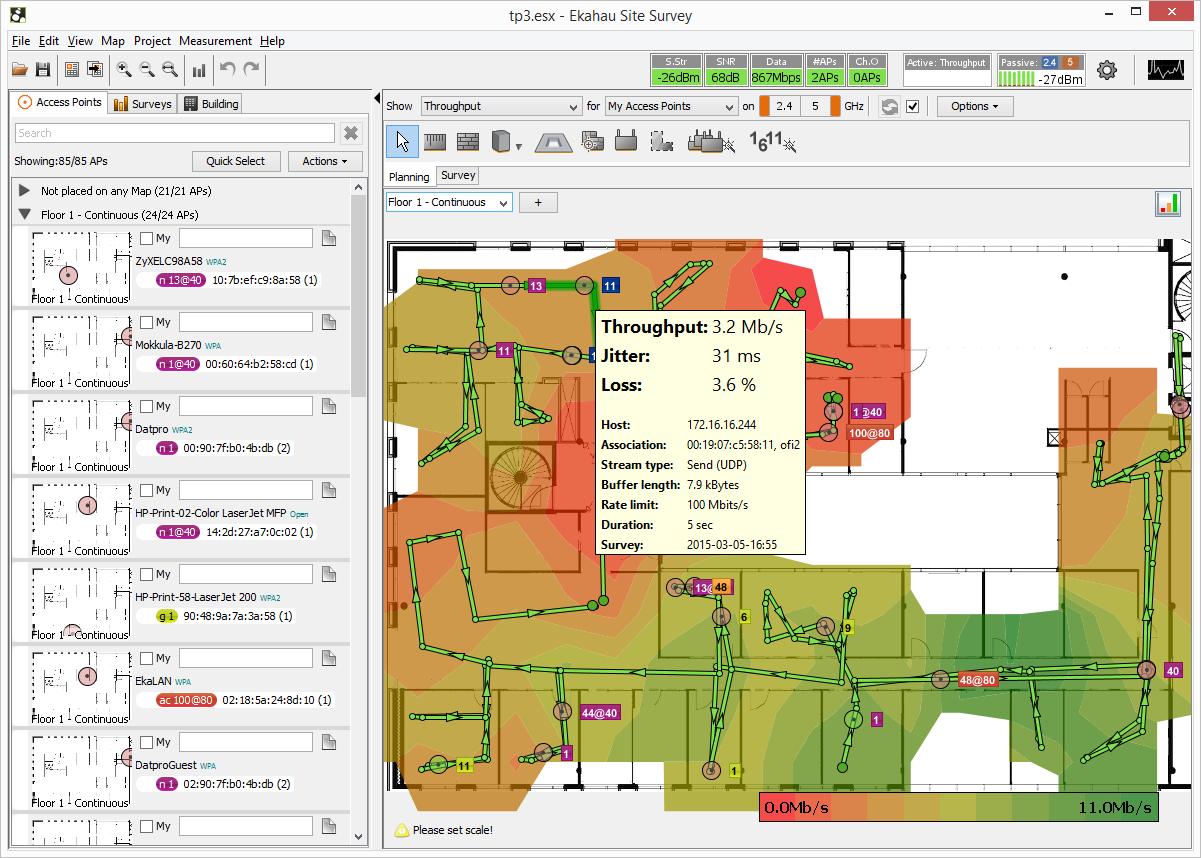
\includegraphics[scale=.38]{figuras/Ekahau-HeatMapper.png}
	}{
		\Fonte{\citeonline{Ekahau2019}.}
	}
\end{figure}

\subsubsection{Acrylic Wi-Fi Heatmaps}
\label{subsubsec:acrylic-wifi-heatmaps}

O Acrylic Wi-Fi Heatmaps consiste de uma ferramenta avançada de análise de rede sem fio para obter uma visão detalhada do cenário \textit{wireless} ao redor. O Acrylic Wi-Fi Heatmaps pode analisar tanto o espectro de frequência de 2.4 GHz quanto o de 5 GHz e gerar mapas de calor detalhados e relatórios em uma variedade de formatos de arquivo comum (Word, CSV, KMZ) \cite{Netspot2019}. 

O gráfico de cobertura  de sinal gerado por esta ferramenta de software (ilustrado na \autoref{fig:acrylic}) pode ser baseado tanto em mapas online, bem como em mapas importados pelo usuário. O Acrylic Wi-Fi Heatmaps torna possível editar os mapas gerados, que é algo que os profissionais podem apreciar. O \textit{software} está disponível gratuitamente para experimentação limitada, tendo a opção de compra com todas as funcionalidades liberadas.

\begin{figure}[H]
	\centering
	\Caption{\label{fig:acrylic}Tela de geração de mapas de calor do Acrylic Wi-Fi Heatmaps.}	
	\UECEfig{}{
		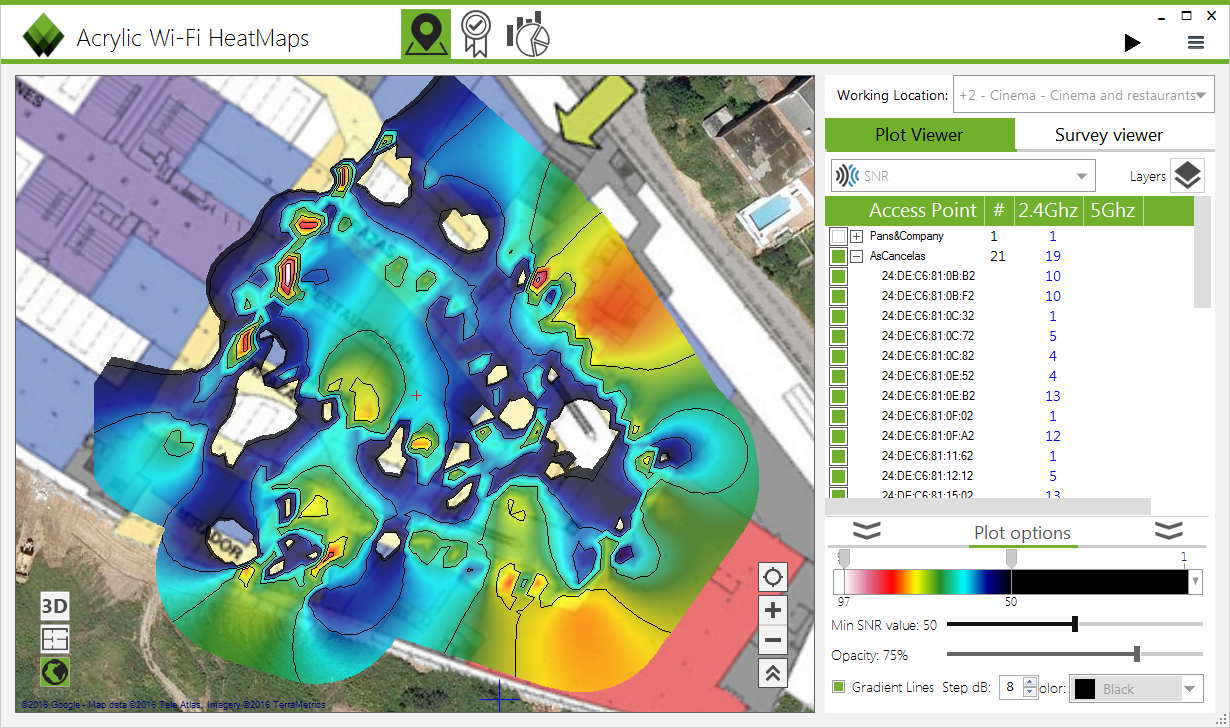
\includegraphics[scale=.28]{figuras/Acrylic-Wi-Fi-Heatmaps.png}
	}{
		\Fonte{\citeonline{Netspot2019}.}
	}
\end{figure}

\subsubsection{VisiWave Site Survey}
\label{subsubsec:visiwave}

O VisiWave Site Survey destina-se especialmente a inspeções de larga escala, como pode ser visto na \autoref{fig:visiwave}, sendo capaz de fornecer três métodos eficazes para a captura de dados: um ponto de cada vez; caminhadas contínuas pela área de pesquisa e posicionamento GPS (do inglês, \textit{Global Positioning System}) para levantamentos ao ar livre. 

É possível criar relatórios personalizados ou reutilizar modelos de relatórios para visualizar sua cobertura ou visualizar interativamente os dados de cobertura no Google Earth\footnote{Google Earth é um programa de computador desenvolvido e distribuído pela empresa estadunidense do Google cuja função é apresentar um modelo tridimensional do globo terrestre, construído a partir de mosaico de imagens de satélite obtidas de diversas fontes.} \cite{Netspot2019}. O VisiWave Site Survey suporta a maioria dos adaptadores de rede Wi-Fi, e não requer nenhum componente de \textit{hardware} especial para funcionar.
\newpage
\begin{figure}[H]
	\centering
	\Caption{\label{fig:visiwave}Tela de geração de mapas de calor do VisiWave Site Survey.}	
	\UECEfig{}{
		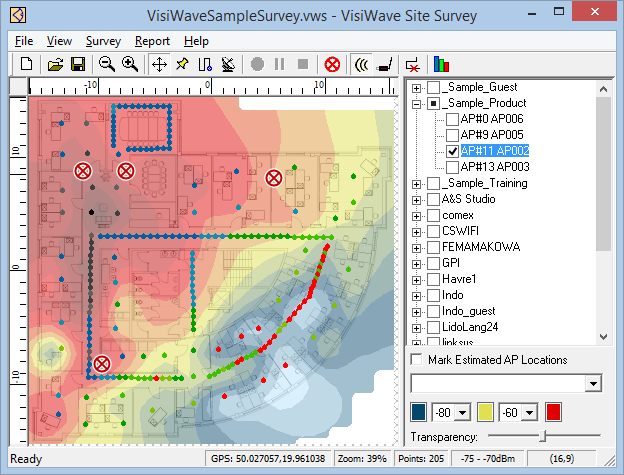
\includegraphics[scale=.64]{figuras/VisiWave-Site-Survey.png}
	}{
		\Fonte{\citeonline{Netspot2019}.}
	}
\end{figure}

\subsubsection{AirMagnet Survey PRO}
\label{subsubsec:airmagnet-pro}

O AirMagnet Survey PRO pode criar um mapa de calor de leitura fácil para sinal/ruído, taxa de transferência de LAN sem fio, taxas de dados, taxas de repetição e as perdas de pacotes da rede, aliado com uma interface gráfica visualmente rica em opções (\autoref{fig:airmagnet-pro}). Este \textit{software} suporta todos os padrões de rede Wi-Fi e possui suporte a um grande número de recursos \cite{Netspot2019}.

\begin{figure}[H]
	\centering
	\Caption{\label{fig:airmagnet-pro}Tela de geração de mapas de calor do AirMagnet Survey PRO.}	
	\UECEfig{}{
		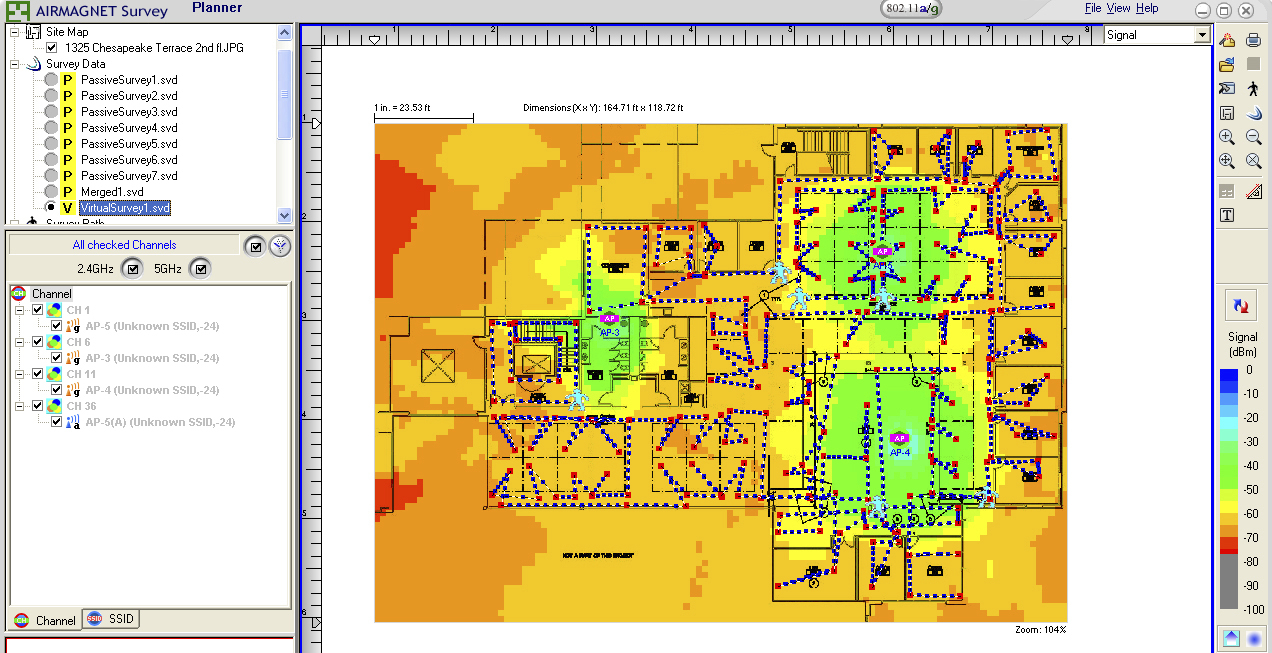
\includegraphics[scale=.38]{figuras/AirMagnet-Survey-PRO.jpg}
	}{
		\Fonte{\citeonline{Netspot2019}.}
	}
\end{figure}

\subsubsection{Xirrus Wi-Fi Inspector}
\label{subsubsec:xirrus-wifi}

O Xirrus Wi-Fi Inspector é um \textit{software} de análise direcionado principalmente para usuários que frequentemente acessam a Internet utilizando computadores portáteis e desejam um método fácil de encontrar redes Wi-Fi, disponível em versão grátis e paga, e com uma interface gráfica amigável e simples (\autoref{fig:xirrus-wifi}). Além de mostrar o SSID, velocidade e o tipo de segurança de cada rede disponível, o programa ainda indica a distância de cada ponto de acesso em relação ao usuário e permite realizar uma série de testes que verificam tanto a velocidade da conexão quanto sua estabilidade.

\begin{figure}[H]
	\centering
	\Caption{\label{fig:xirrus-wifi}Tela principal do Xirrus Wi-Fi Inspector.}	
	\UECEfig{}{
		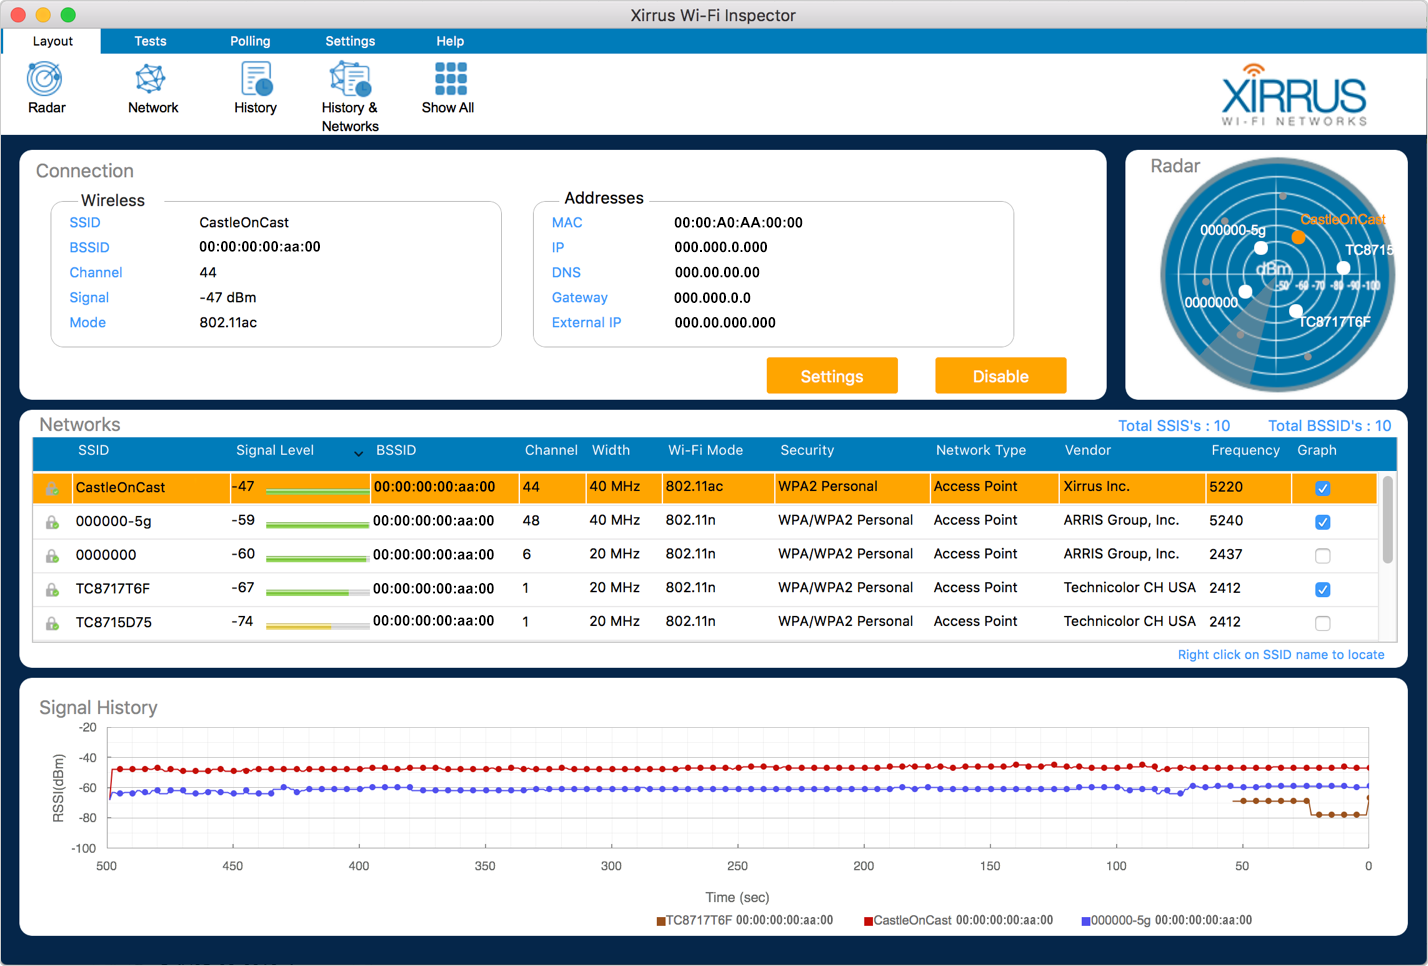
\includegraphics[scale=.3]{figuras/inspector_layout_Riverbed.png}
	}{
		\Fonte{\citeonline{Xirrus}.}
	}
\end{figure}
	\chapter{Metodologia e Resultados}
\label{cap:metodologia-e-resultados}

O trabalho foi desenvolvido de acordo coma as etapas apresentados no fluxograma da \autoref{fig:flux-metodologia}.

Visando uma melhor execução, a metodologia \textit{site survey} foi implementada seguindo as respectivas fases:
\begin{compactitem}
	\item \textbf{Reconhecimento do local:} o Bloco Didático foi inspecionado em busca de características estruturais que possam vir a influenciar na propagação do sinal Wi-Fi.
	
	\item \textbf{Coleta de dados:} com o auxílio de \textit{softwares}, medidas de potência foram capturadas em diversos pontos do prédio e posteriormente marcados na planta baixa do prédio.
	
	\item \textbf{Tratamento dos dados:} depois de coletados, os dados foram tratados a fim de filtrar quais seriam úteis para a proposta do trabalho.
	
	\item \textbf{Geração dos mapas de calor:} representações gráficas da cobertura de rádio do ponto de acesso foram feitas para demonstrar onde o sinal sofria maiores perdas.
\end{compactitem}

\begin{figure}[H]
	\centering
	\Caption{\label{fig:flux-metodologia}Fluxograma da metodologia do trabalho.}	
	\UECEfig{}{
		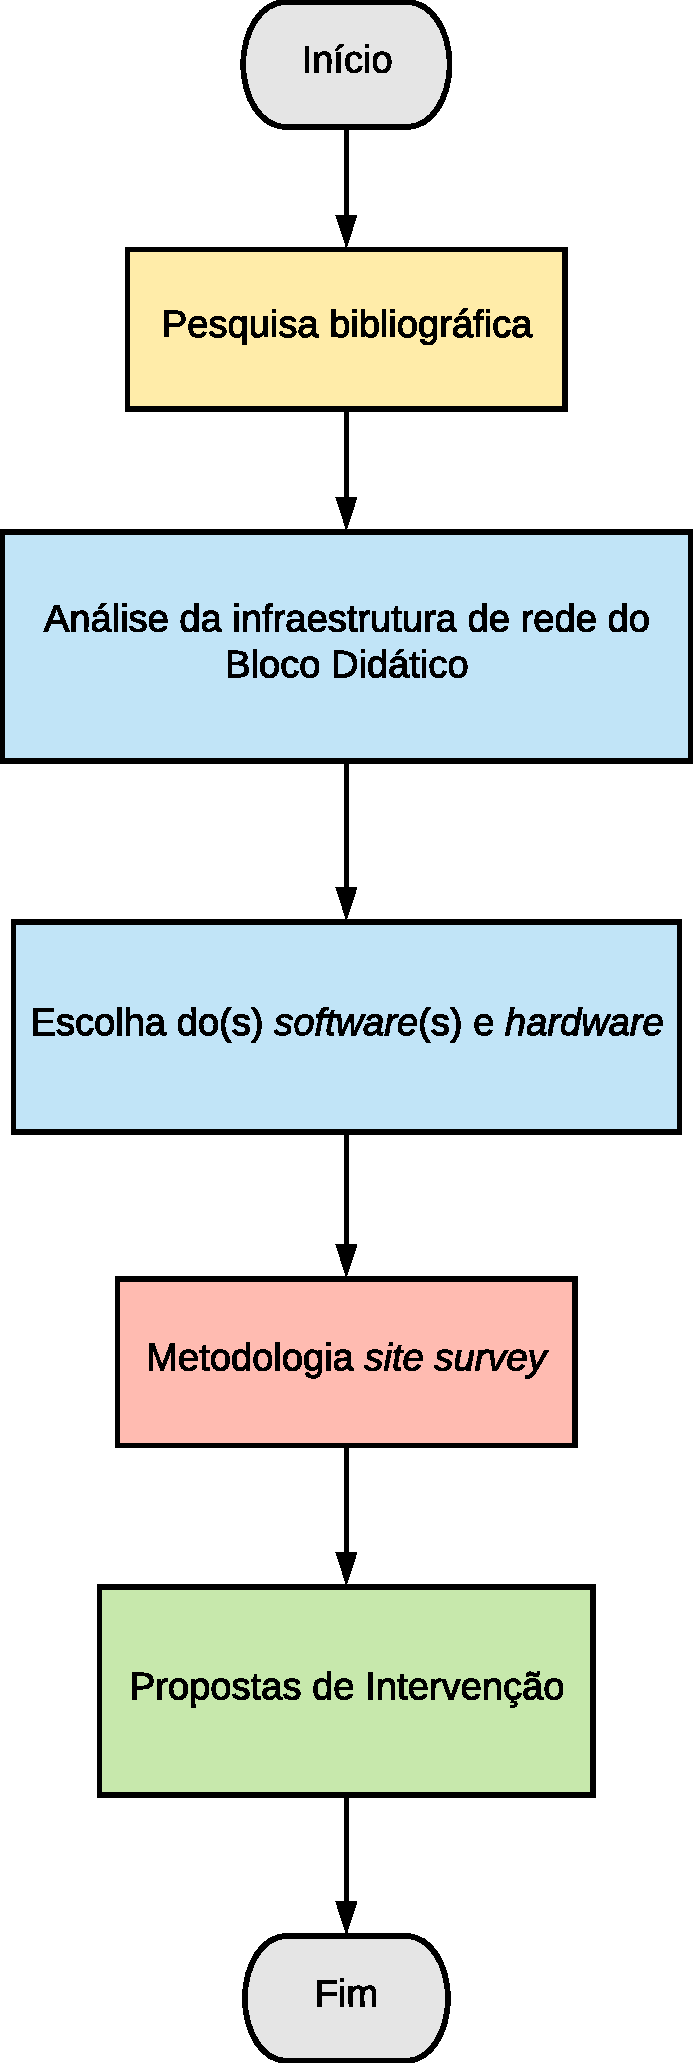
\includegraphics[scale=.36]{figuras/Novo_Fluxograma_Metodologia_TCC.pdf}
	}{
		\Fonte{Autor.}%
	}	
\end{figure}

\section{Estudo de Caso}
\label{sec:estudo-de-caso}

O Instituto Federal de Educação, Ciência e Tecnologia do Ceará conta com 32 \textit{campi} em funcionamento distribuídos por todo o estado. O \textit{campus} de Tauá do IFCE, foi inaugurado em 20 de novembro de 2009. O \textit{campus} abrange principalmente os municípios de Aiuaba, Arneiroz, Quiterianópolis e Parambu, e recebe alunos de várias outras regiões por meio do Sistema de Seleção Unificada (SISU) do Ministério da Educação (MEC) \cite{ifceTaua2019}.

O \textit{campus} Tauá oferta atualmente os cursos técnicos integrados em Redes de Computadores e Agropecuária e os cursos superiores de Tecnologia de Telemática e Licenciatura em Letras com habilitação em Inglês e Português. No semestre letivo 2019.1, o \textit{campus} conta com mais de 400 alunos matriculados \cite{ifceTaua2019}.

A estrutura física do IFCE Tauá pode ser dividida em duas partes principais: a primeira conta com a instalação original do projeto (inaugurada em 2009), onde está inserida a administração, os laboratórios e a biblioteca; a segunda representa o Bloco Didático, inaugurado em 5 de julho de 2016, o qual abriga oito salas de aula, a coordenadoria de cursos e os laboratórios de informática e eletromagnetismo. No total, o Bloco Didático do \textit{campus} Tauá ocupa uma área construída de aproximadamente 2000 $m^{2}$. O presente trabalho foi desenvolvido no Bloco Didático da instituição, já que este concentra as salas de aula, o que resulta em um grande fluxo de pessoas pela área, principalmente de alunos.

O \textit{campus} Tauá conta com diversas atividades de pesquisa, extensão e ensino exercidas por discentes, docentes e técnicos. Assim, a instituição, visando atender a comunidade acadêmica, disponibiliza uma infraestrutura de rede sem fio.

Na \autoref{fig:vista-campus}, tem-se uma visão total da área do \textit{campus}, delimitada pela marcação em vermelho, que é composto pelo bloco inicial do projeto de 2009, destacado em azul, pelo Bloco Didático, em verde, e pela quadra poliesportiva localizada imediatamente acima deste último prédio.

\begin{figure}[H]
	\centering
	\Caption{\label{fig:vista-campus}Visão aérea do IFCE \textit{campus} Tauá.}	
	\UECEfig{}{
		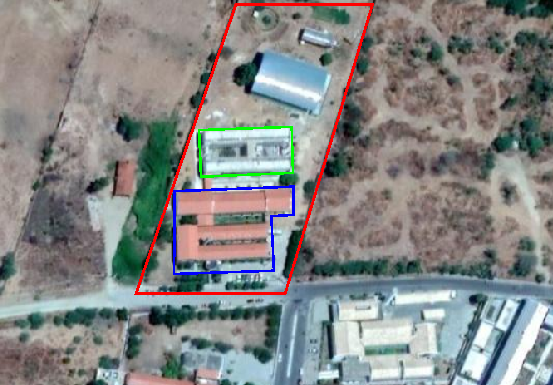
\includegraphics[scale=1]{figuras/ifce-taua-maps.pdf}
	}{
		\Fonte{\citeonline{GoogleMaps}.}
	}	
\end{figure}

%\subsection{Infraestrutura da rede sem fio do IFCE Tauá}
%\label{subsec:infraestrutura-wireless}

A instituição conta com uma infraestrutura de rede sem fio com vários pontos de acesso distribuídos em diversos locais de sua área. No bloco 1 (bloco inicial) encontram-se a maior concentração de pontos de acesso, destinados a suprir as necessidades de conexão à Internet do setor administrativo e de pesquisas desenvolvidas no \textit{campus}. Para todo o espaço do Bloco Didático, há a presença de dois pontos de acesso: um destinado aos estudantes e o outro aos professores, ambos localizados na sala de coordenação situada no primeiro andar, indicados pelos marcadores conforme ilustra a \autoref{fig:local-ap}. Para o térreo, não existe pontos de acesso instalados. Todos os pontos de acesso no \textit{campus} são protegidos com senhas de acesso alfanuméricos.

\begin{figure}[H]
	\centering
	\Caption{\label{fig:local-ap}Localização dos pontos de acesso no 1º andar do Bloco Didático.}	
	\UECEfig{}{
		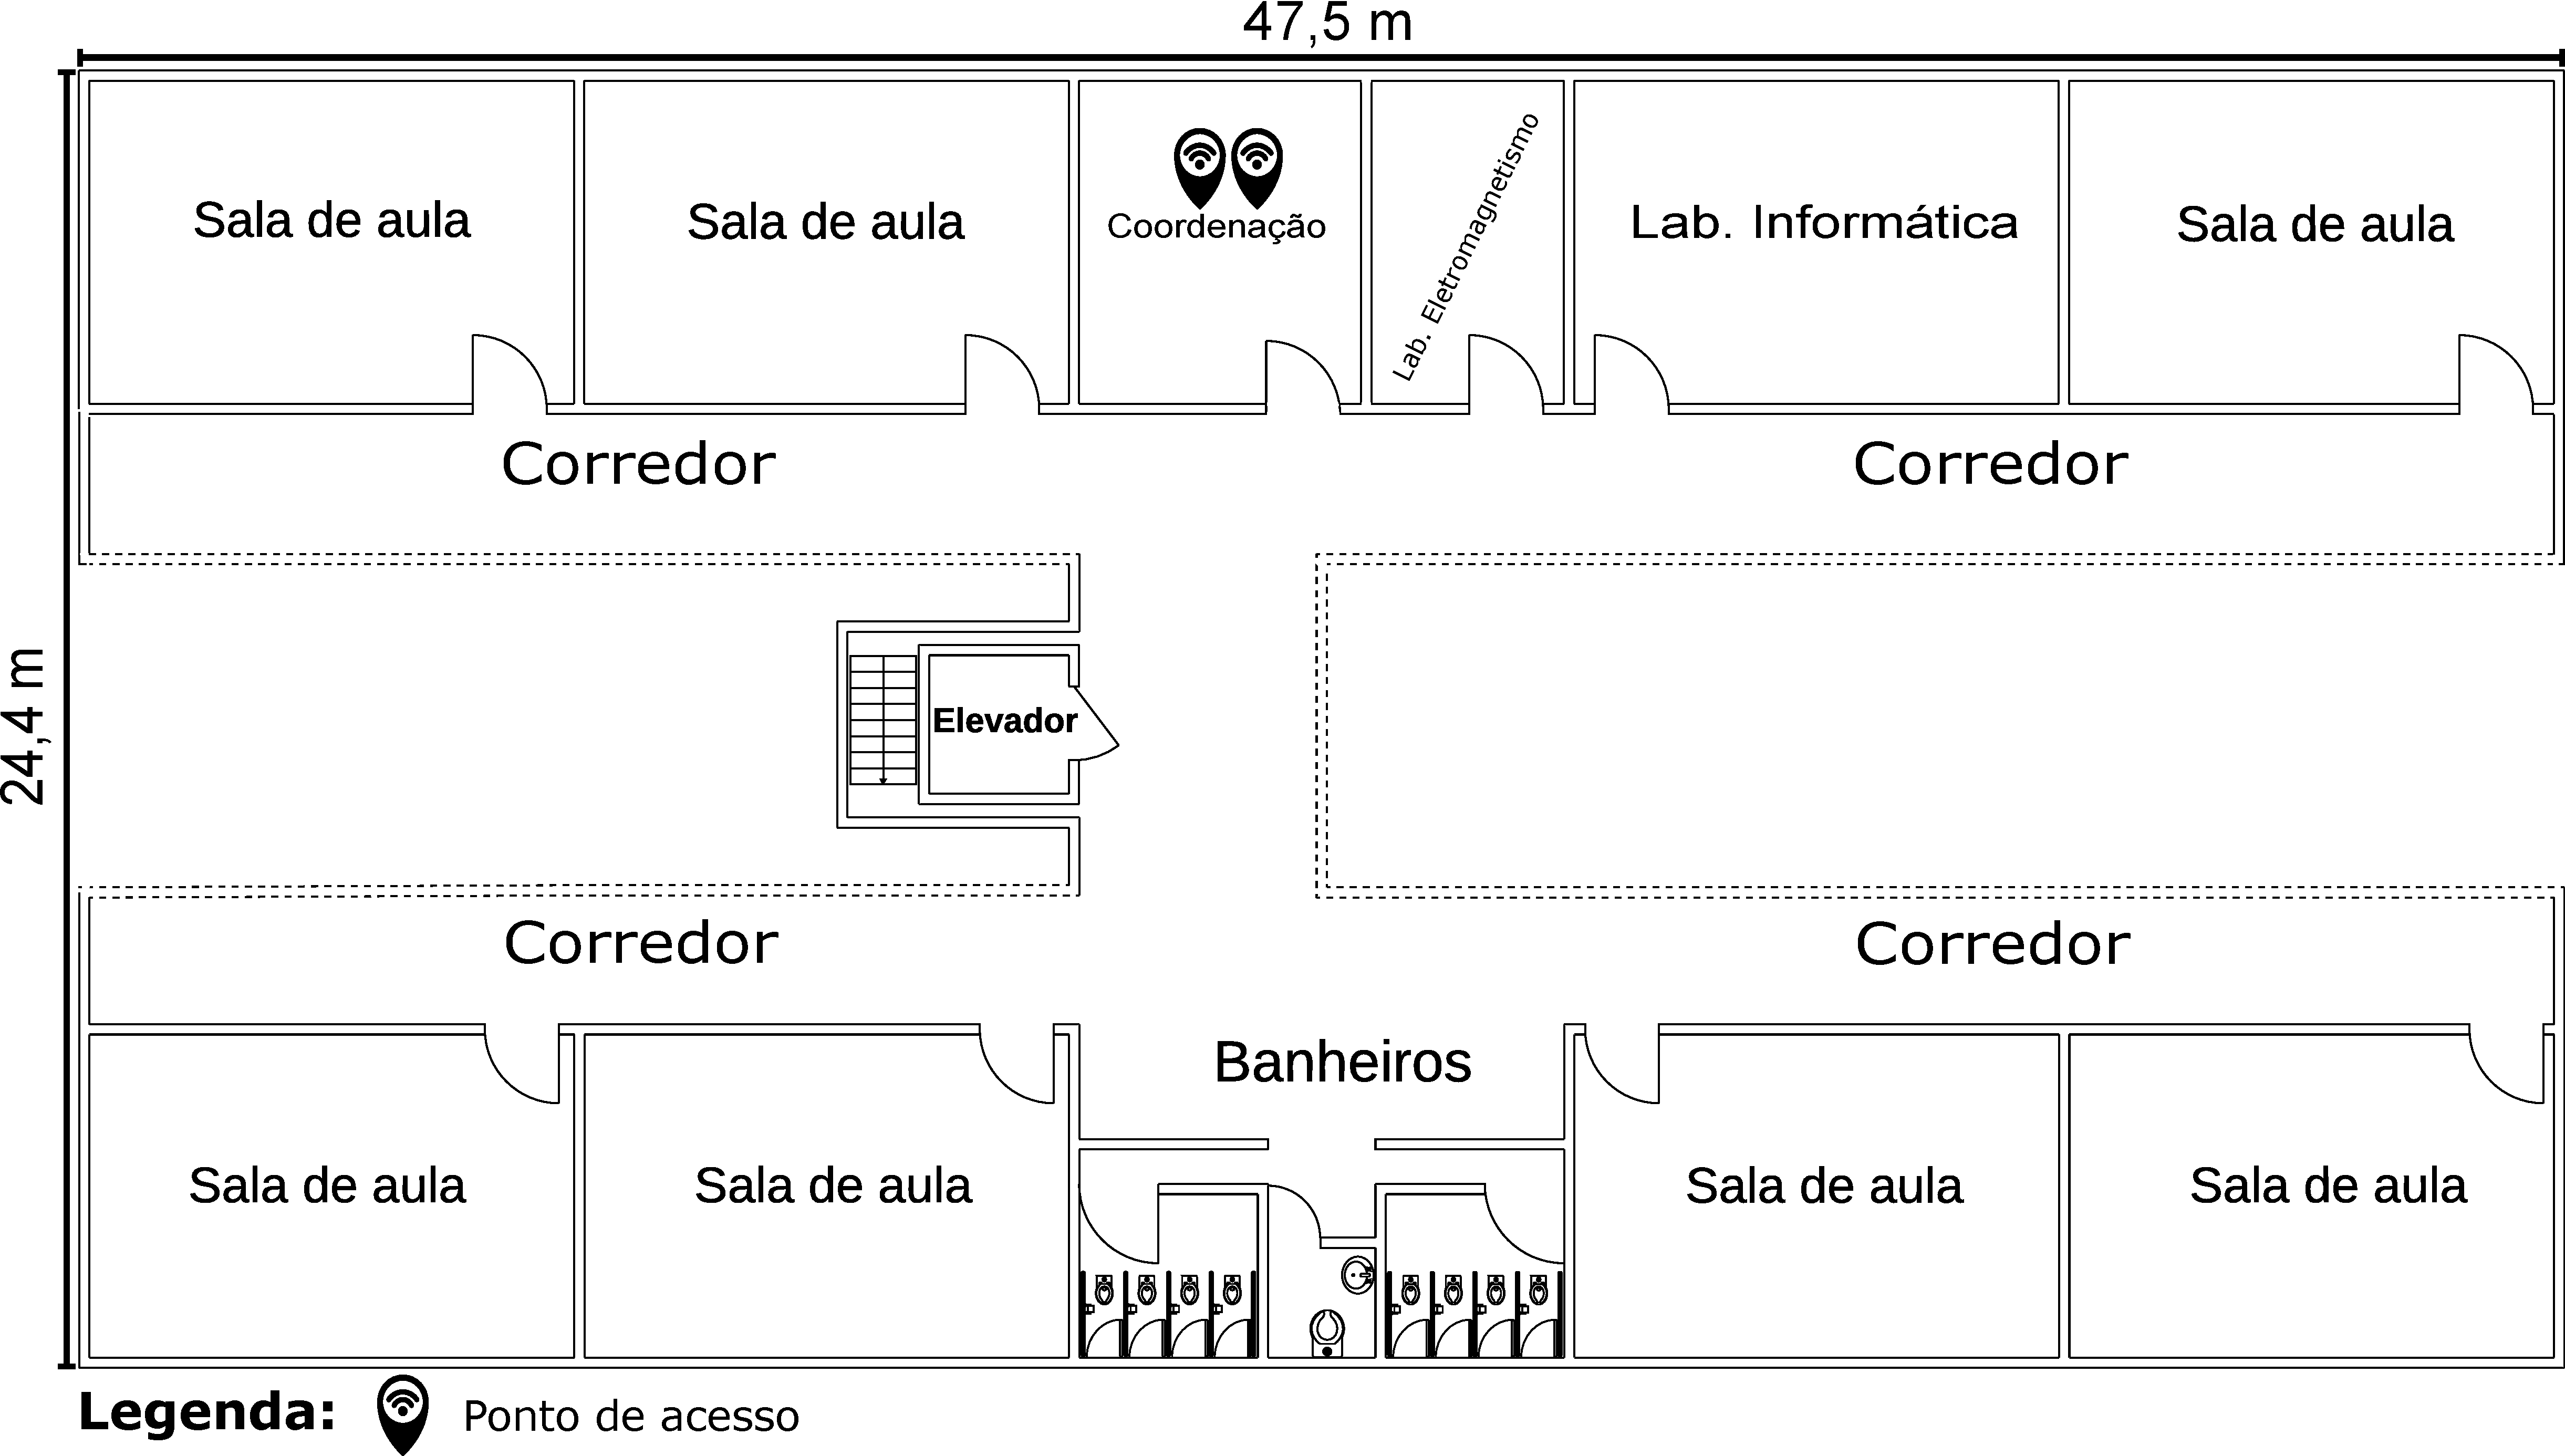
\includegraphics[scale=.185]{figuras/APs_Bloco_Andar_2_Perimetro.pdf}
	}{
		\Fonte{Autor.}
	}	
\end{figure}

A Internet disponibilizada no IFCE Tauá é acessível tanto para aqueles que estudam na instituição ou trabalham, como também para visitantes, desde que tenham a senha de acesso. A rede sem fio é dividida de forma a atender cada setor que compõe a organização institucional do \textit{campus}. Isso quer dizer que para os frequentadores da biblioteca existe uma rede específica para eles; para os professores da mesma forma. No entanto, não há restrições para que cada categoria de usuários utilize sua rede própria, cada usuário é livre para associar-se a qualquer ponto de acesso disponível, desde que tenha autorização para tal.

As configurações que podem ser encontradas nos pontos de acesso variam de equipamentos que operam na frequência de 2.4 GHz chegando até ao modo \textit{dual band}. \textcolor{blue}{Especificamente, os pontos de acesso empregados na conexão sem fio à Internet no Bloco Didático e também em quase todo o restante do \textit{campus} Tauá são do modelo AC1750 Wireless Dual Band Gigabit Router Archer C7 (\autoref{fig:archer-c7}) da marca comercial TP-Link. Este equipamento pode trabalhar, simultaneamente, nas bandas de 2.4 GHz e 5 GHz, suas especificações \textit{wireless} podem ser vistas na \autoref{tab:roteador-tp-link}.}

\begin{figure}[H]
	\centering
	\Caption{\label{fig:archer-c7}AC1750 Wireless Dual Band Gigabit Router Archer C7.}	
	\UECEfig{}{
		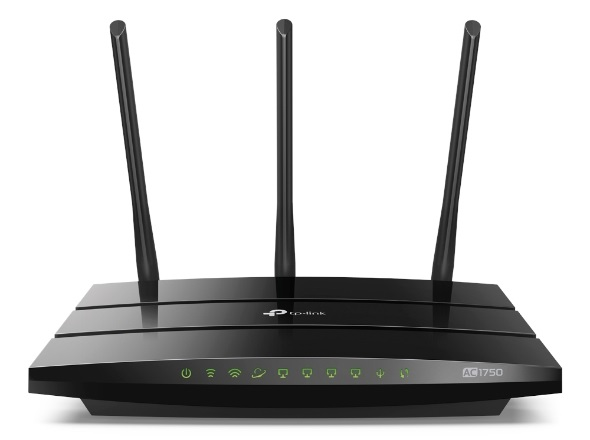
\includegraphics[scale=.38]{figuras/TP-Link_Archer_C7.jpg}
	}{
		\Fonte{\citeonline{archerc72019}.}
	}	
\end{figure}

\begin{table}[H]
	\Caption{\label{tab:roteador-tp-link}Especificações técnicas do ponto de acesso Archer C7.}%
	\IBGEtab{}{%
		\begin{tabular}{lc}
			\toprule
			\multicolumn{1}{c}{Característica do dispositivo} & \multicolumn{1}{c}{Descrição} \\
			\toprule %\midrule
			
			Padrão \textit{Wireless} & \begin{tabular}[c]{@{}l@{}} IEEE 802.11ac/n/a 5 GHz\\ IEEE 802.11b/g/n 2.4 GHz\end{tabular} \\
			
			Frequência de Operação & 5 GHz e 2.4 GHz \\
			
			Taxa de Sinal & 5 GHz: Até 1300 Mbps, 2.4 GHz: Até 450 Mbps \\
			
			Sensibilidade de Recepção & \begin{tabular}[c]{@{}l@{}}5 GHz:\\ 11a 6 Mbps: -96 dBm, 11a 54 Mbps: -79dBm\\ 11ac HT20: -71 dBm, 11ac HT40: -66 dBm, 11ac HT80: -63 dBm\\ 2.4 GHz:\\ 11g 54 Mbps: -77 dBm, 11n HT20: -74 dBm, 11n HT40: -72 dBm\end{tabular} \\
			
			Potência de Transmissão & \begin{tabular}[c]{@{}l@{}}CE: <20 dBm (2.4 GHz), \textless{}23 dBm (5 GHz)\\ 
				FCC: <30 dBm (2.4 GHz e 5 GHz)\end{tabular} \\

			\bottomrule
		\end{tabular}%
	}{%
		\Fonte{\citeonline{archerc72019}.}%
		%\citeonline[p. ~465]{lott2001ieee}; \apudonline[p.~73]{lott2001ieee}{geier2002}
		\Nota{{HT20, HT40 e HT80 correspondem, respectivamente, aos canais de 20 MHz, 40 MHz e 80 MHz.}}
	}%
\end{table}

\section{Materiais utilizados}
\label{materiais-uyilizados}

\subsection{Software}
\label{subsec:softwares-utiliados}

Para que sejam realizados os testes iniciais de \textit{site survey} numa rede sem fio é necessário a utilização de \textit{software(s)} dedicado(s) que permita(m) capturar as informações necessárias que possibilitam avaliar o funcionamento da rede. Neste trabalho foram utilizados dois \textit{softwares}: um para a visualização das redes disponíveis no local alvo (Xirrus Wi-Fi Inspector) e o outro para a geração dos mapas de intensidade de sinal (Ekahau HeatMapper). \textcolor{blue}{A escolha por estes programas se deu pelo fato de serem gratuitos, estáveis, e por não exigirem elevados recursos computacionais.}

Além de ser gratuito, o Xirrus Wi-Fi Inspector apresenta uma interface amigável para a visualização das redes Wi-Fi disponíveis. Além disso, a página principal dele exibe quatros campos diferentes que podem ser expandidos para uma visualização mais detalhada: \textit{Radar}, \textit{History}, \textit{Connection} e \textit{Networks}. Cada um possui algumas funções específicas, mas para a proposta deste trabalho, apenas o campo \textit{Networks} foi explorado, o qual exibe as informações minuciosas das redes detectadas em determinada área (\autoref{fig:software-xirrus}).

\begin{figure}[H]
	\centering
	\Caption{\label{fig:software-xirrus}Tela de \textit{Networks} do Xirrus Wi-Fi Inspector.}	
	\UECEfig{}{
		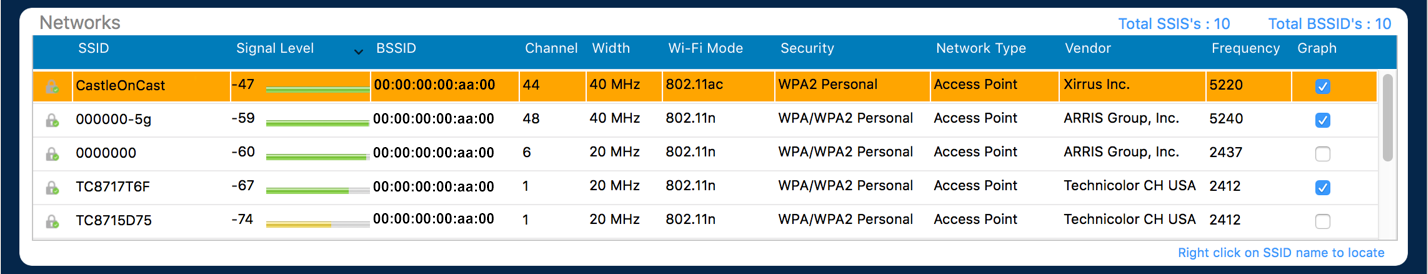
\includegraphics[scale=.41]{figuras/inspector_layout_Riverbed_Networks.png}
	}{
		\Fonte{Autor.}
	}	
\end{figure}

Na janela \textit{Networks} são apresentadas algumas informações dos pontos de acessos descobertos, descritas a seguir:

\begin{compactitem}
	\item \textbf{SSID}: representa o nome da rede sem fio, usado para identificar a mesma, é necessário para associar-se ao ponto de acesso.
	\item \textbf{\textit{Signal Level}:} apresenta a potência do sinal recebido do ponto de acesso em dBm.
	\item \textbf{\textit{Wi-Fi Mode}:} apresenta a versão do padrão 802.11 configurado no ponto de acesso.
	\item \textbf{\textit{Security}:} exibe o protocolo de segurança utilizado pela rede sem fio.
	\item \textbf{\textit{Vendor}:} mostra qual o nome do fabricante do equipamento.
	\item \textbf{BSSID (do inglês, \textit{Basic Service Set Identifier})}: mostra o endereço físico do dispositivo da rede Wi-Fi, que no caso é o endereço MAC (do inglês, \textit{Media Access Control}).
	\item \textbf{\textit{Channel}:} exibe o canal de frequência que o ponto de acesso está utilizando.
	\item \textbf{\textit{Frequency}:} representa a frequência utilizada por um determinado ponto de acesso, podendo ser 2.4 GHz ou 5 GHz.
	\item \textbf{\textit{Network Type}:} exibe o tipo de operação do dispositivo que opera a rede Wi-Fi, seja ponto de acesso ou \textit{ad hoc}.
	\item \textbf{\textit{Graph}:} caixa de seleção para ativar/desativar a representação gráfica do nível de sinal da rede Wi-Fi ao longo do tempo.
\end{compactitem}
	
Já para a criação de mapas de calor dos sinais de radiofrequência, o programa utilizado foi o Ekahau HeatMapper. Com ele é possível descobrir a cobertura de uma rede Wi-Fi padrão 802.11n/b/g a partir da visualização do mapa de calor obtido na coleta de dados em diversos pontos espalhados pelo local.

O programa possibilita ao usuário escolher um arquivo de seu computador que representa a planta baixa do ambiente de interesse, para assim marcar os pontos onde as medidas de potência foram capturadas e posteriormente a coloração. Cada cor exibida pelo \textit{software} significa a intensidade de potência do sinal recebido em certo ponto, variando do verde (sinal forte) até o vermelho (sinal fraco). Além disso, as marcações retilíneas em verde indicam o percurso feito pelo \textit{notebook} durante o mapeamento enquanto os pontos apontam o local de coleta de medidas. %Todos esses detalhes são ilustrados pela \autoref{fig:ekahau}.

%\begin{figure}[H]
%	\centering
%	\Caption{\label{fig:software-ekahau}Geração do mapa de calor no Ekahau HeatMapper.}	
%	\UECEfig{}{
%		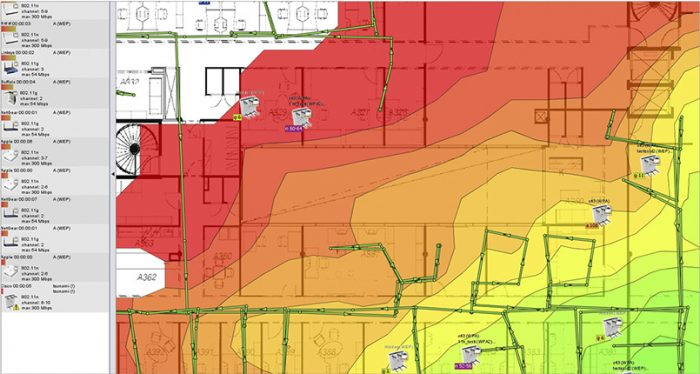
\includegraphics[scale=.5]{figuras/ekahau-heatmapper.jpg}
%	}{
%		\Fonte{\citeonline{Ekahau2019}.}
%	}	
%\end{figure}

\subsection{Hardware}
\label{subsec:equipamento-utilizado}

Para poder dar início nas medições dos níveis de potência foi utilizado o \textit{notebook} Positivo Master N40i (\autoref{fig:notebook}) com os \textit{softwares} Xirrus Wi-Fi Inspector e Ekahau HeatMapper instalados e configurados. As especificações do computador podem ser visualizadas na \autoref{tab:carac-notebook}.

\begin{figure}[H]
	\centering
	\Caption{\label{fig:notebook}Notebook Positivo Master N40i.}	
	\UECEfig{}{
		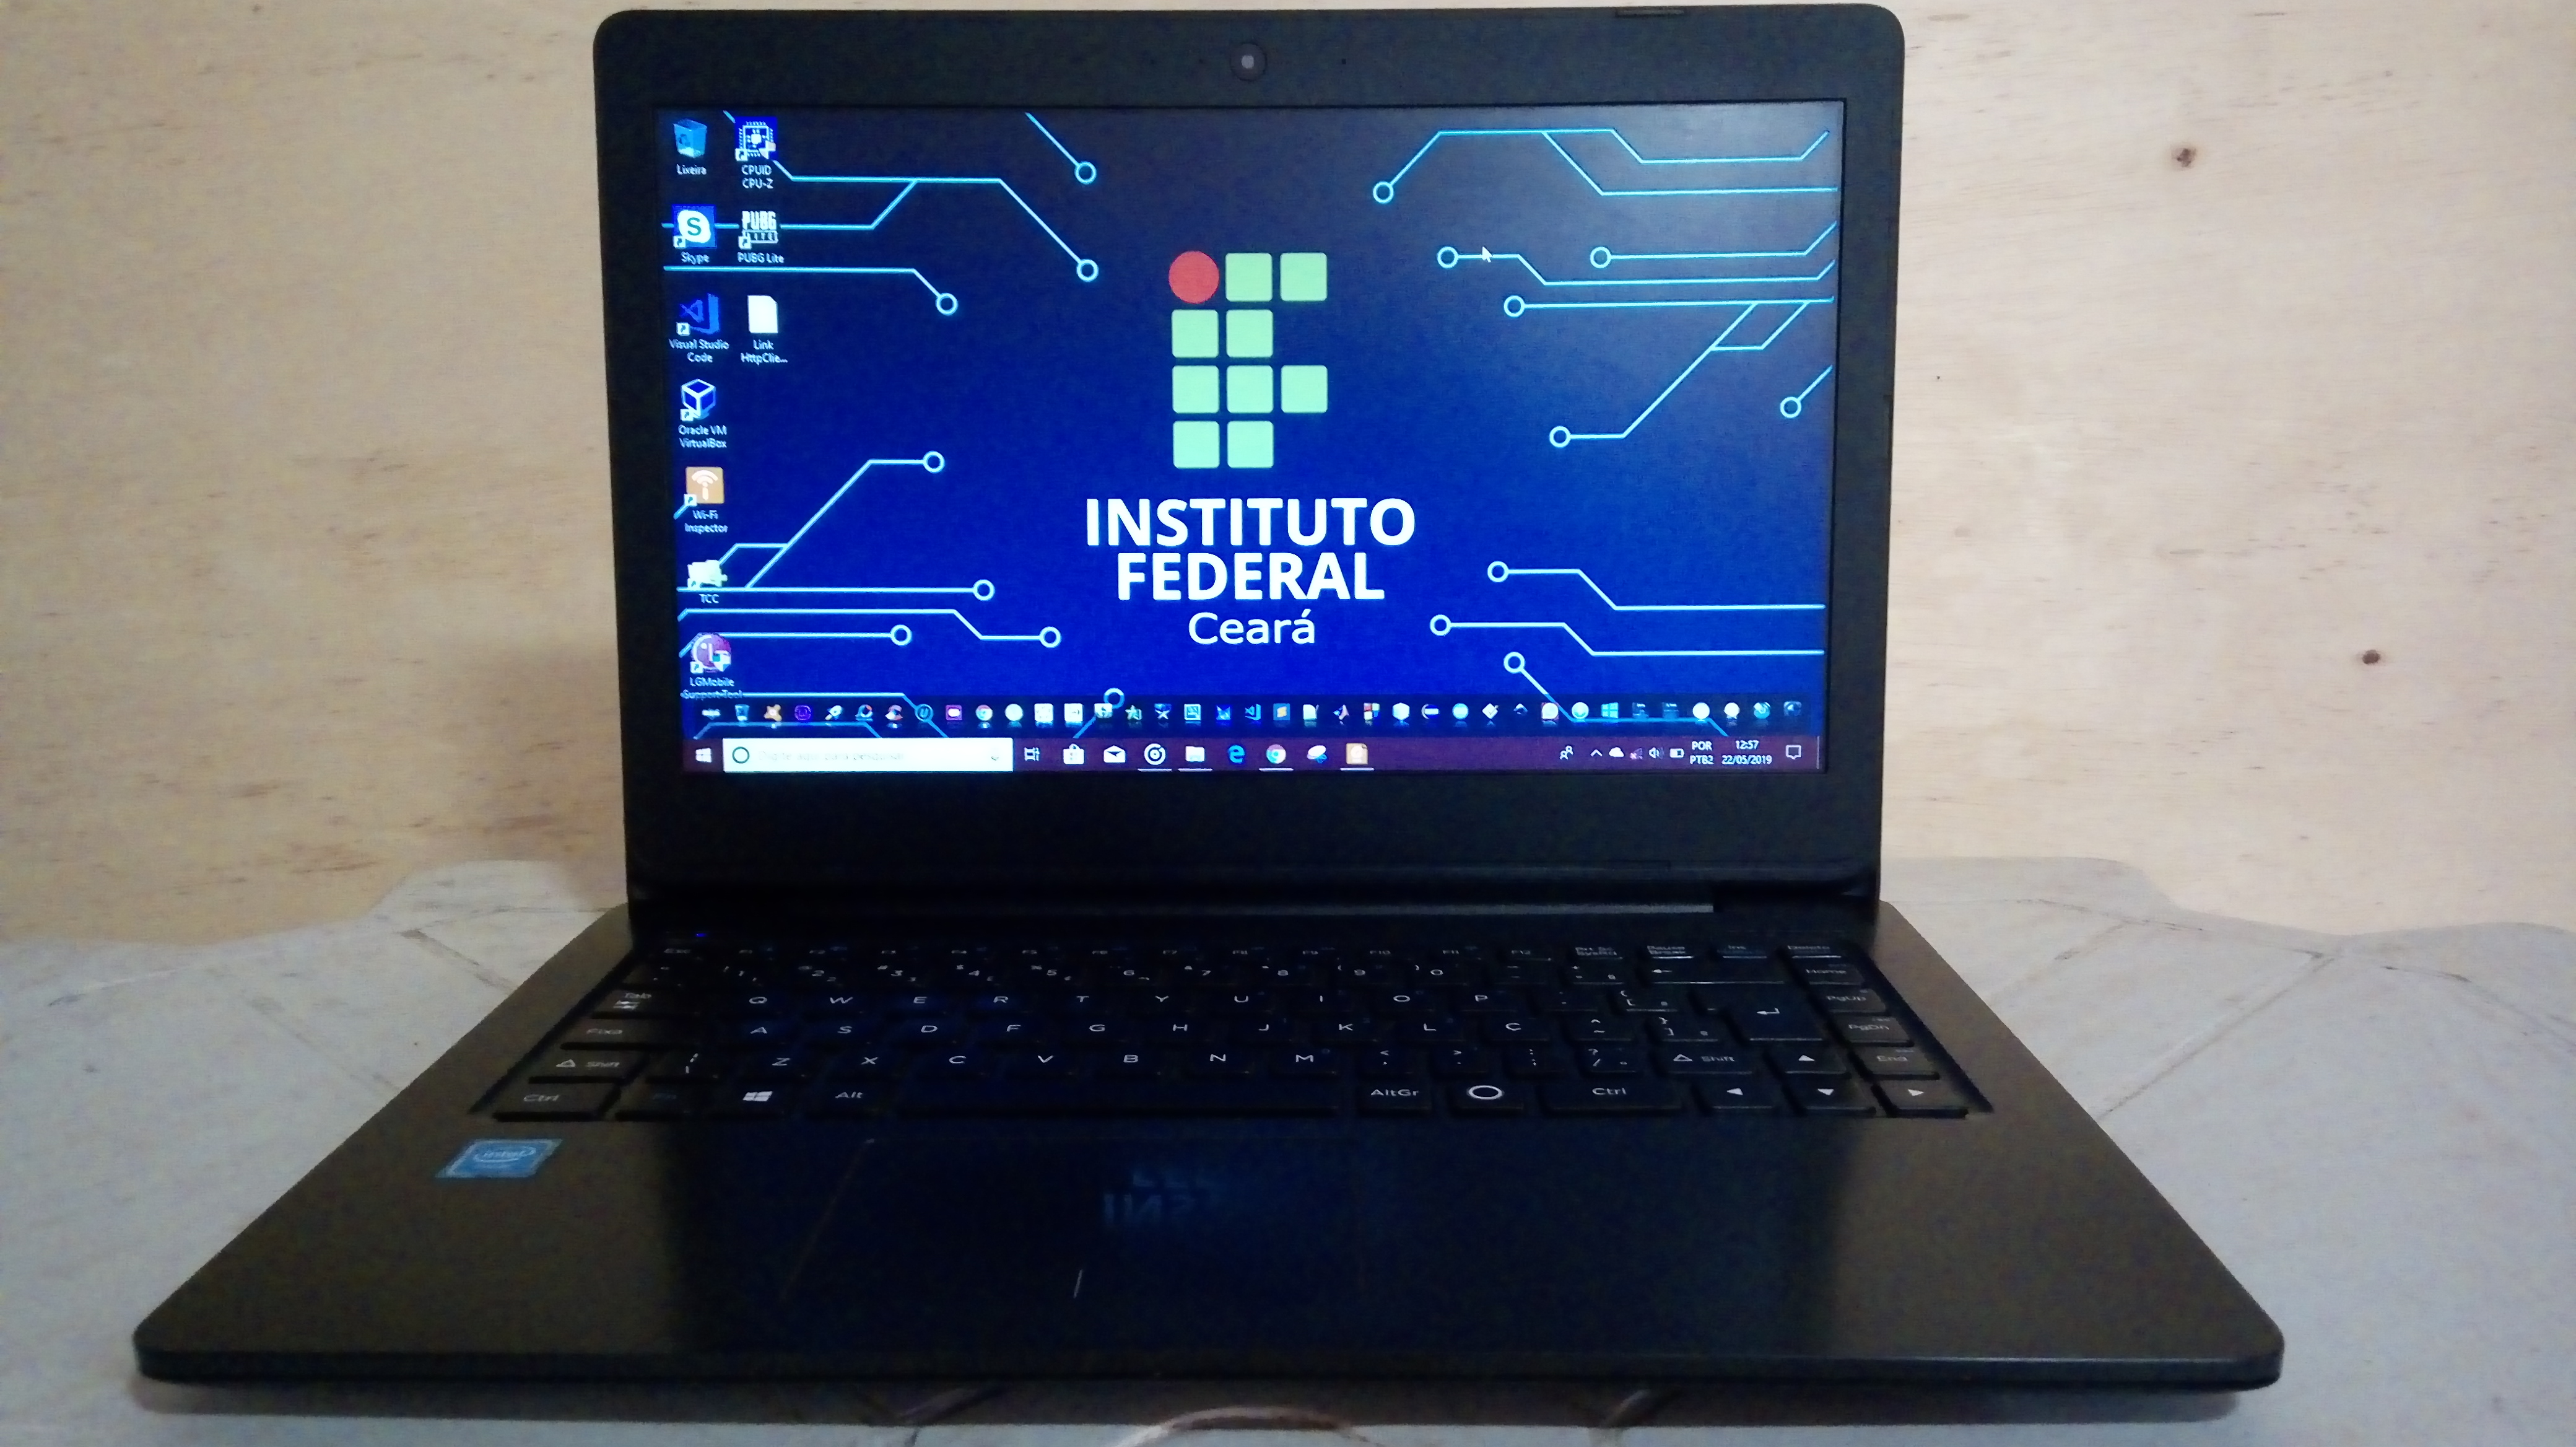
\includegraphics[scale=.1]{figuras/notebook.jpg}
	}{
		\Fonte{Autor.}%
	}	
\end{figure}

\begin{table}[H]
	\Caption{\label{tab:carac-notebook}Especificações do \textit{notebook} utilizado.}%
	\IBGEtab{}{%
		\begin{tabular}{ll}
			\toprule
			\multicolumn{1}{c}{Características do sistema} & \multicolumn{1}{c}{Descrição} \\
			\toprule %\midrule
			Modelo & Positivo Master N40i \\
			
			Sistema Operacional & Windows 10 Pro 64 bits \\
			
			RAM & 4 GB \\
			
			Processador & Intel Celeron N3060 @1.60GHz (2 CPUs) \\
			
			Placa de rede & Intel Dual Band Wireless-AC 3160 \\
			\bottomrule
		\end{tabular}%
	}{%
		\Fonte{Autor.}%
	}%
\end{table}

\section{Execução do site survey}
\label{sec:execucao-site-survey}

O processo de \textit{site survey} desenvolvido no IFCE \textit{campus} Tauá, caracterizado como do tipo \textit{indoor}, foi dividido, para uma melhor execução, em quatro etapas que vão desde o início da coleta dos dados em campo até os resultados obtidos, definidas como se segue:

\begin{compactenum}
	\item Reconhecimento do local;
	\item Coleta dos dados;
	\item Tratamento dos dados;
	\item Geração dos mapas de calor.
\end{compactenum}

\subsection{Reconhecimento do local}
\label{subsec:reconhecimento-do-local}

Nesta primeira etapa do \textit{site survey}, após a instalação dos programas no \textit{notebook}, já citados, foi feita uma vistoria em toda a área correspondente ao Bloco Didático do \textit{campus} com a objetivo de verificar a sua infraestrutura física, identificar possíveis pontos para a medição e a presença ou não de fontes de interferências.

O ambiente analisado abrange uma área do tipo \textit{indoor} por conter salas, e também \textit{outdoor} devido ao espaço livre no prédio, como os que estão no térreo. O elevador, localizado no centro do prédio, como pode ser visto na imagem do topo da \autoref{fig:andar1} tem seu uso restrito à pessoas com necessidades especiais. Envolto ao elevador, a escadaria oferece o acesso aos dois pisos da construção. As Figuras \ref{fig:andar1} e \ref{fig:andar2} mostram alguns dos pontos que foram verificados.

\begin{figure}[H]
	\centering
	\Caption{\label{fig:andar1}Alguns dos locais inspecionados no térreo do Bloco didático.}	
	\UECEfig{}{
		\includegraphics[scale=.18]{figuras/Andar01.png}
	}{
		\Fonte{Autor.}%
	}	
\end{figure}

\begin{figure}[H]
	\centering
	\Caption{\label{fig:andar2}Alguns dos locais inspecionados no 1º andar do Bloco Didático.}	
	\UECEfig{}{
		\includegraphics[scale=.12]{figuras/Andar02.png}
	}{
		\Fonte{Autor.}%
	}	
\end{figure}

\subsection{Coleta dos dados}
\label{subsec:coleta-de-dados}

Nesta etapa foi iniciado o procedimento de medição dos níveis de potência, com a finalidade de obter informações das redes sem fio no \textit{campus} Tauá, sobretudo da cobertura das mesmas. O acesso e a utilização da planta baixa do Bloco Didático favoreceram para que fosse possível identificar a localização dos pontos de acesso e a estrutura física da instituição.

No Ekahau HeatMapper foi carregada a imagem da planta baixa do Bloco Didático. Logo após essa configuração, foi iniciada a demarcação dos pontos de medição por todo o local.

As primeiras medições ocorreram nos ambientes do tipo \textit{indoor} do Bloco Didático, o que inclui salas e laboratórios. Após a coleta dos níveis do sinal da rede de toda a parte interna, foi feita a captura na parte externa, como os corredores e locais sociais frequentados pelos estudantes. Em todo o prédio foram primeiramente analisados o térreo, e posteriormente o primeiro.

Para que todos os valores de medição obtidos na coleta fossem os mais precisos possível, foi feita uma comparação entre o ponto da planta baixa no Ekahau HeatMapper e o local da área real. Com isso, toda vez que um ponto de medida foi gerado, se obteve as potências de todas as redes Wi-Fi que estavam ao alcance do \textit{notebook}.

As medições ocorreram em 18 de maio de 2019 (sábado), pelo fato de que nesta data todos os docentes e discentes estariam ausentes do \textit{campus}. Isso contribuiu para que todas as salas e áreas que o Bloco Didático dispõe fossem visitadas e mapeadas.

A \autoref{fig:pontos-andar2} mostra os 62 pontos marcados no térreo do Bloco Didático. Cada ponto vermelho na figura significa um local que foi medido a potência de sinal da rede Wi-Fi. Já a \autoref{fig:pontos-andar1} apresenta todos os 50 pontos que foram medidos no térreo do mesmo prédio. Para cada ponto de medição, um tempo entre 30 e 60 segundos foi gasto com a finalidade de gerar um valor médio para a potência recebida naquele determinado ponto, pois o sinal sem fio sofre com flutuações rápidas, logo seu valor instantâneo pode não condizer com a realidade do local de medição.

\textcolor{blue}{A quantidade de pontos medidos nos dois andares compreende suficientemente toda a área útil do prédio. A localização de cada ponto procurou quantificar a potência do sinal em todos os locais do prédio com diferentes condições arquitetônicas (no interior das salas, dos banheiros, nos corredores) para assim tornar os resultados os mais completos e precisos possíveis.}

\begin{figure}[H]
	\centering
	\Caption{\label{fig:pontos-andar2}Pontos medidos no 1º andar do Bloco Didático.}	
	\UECEfig{}{
		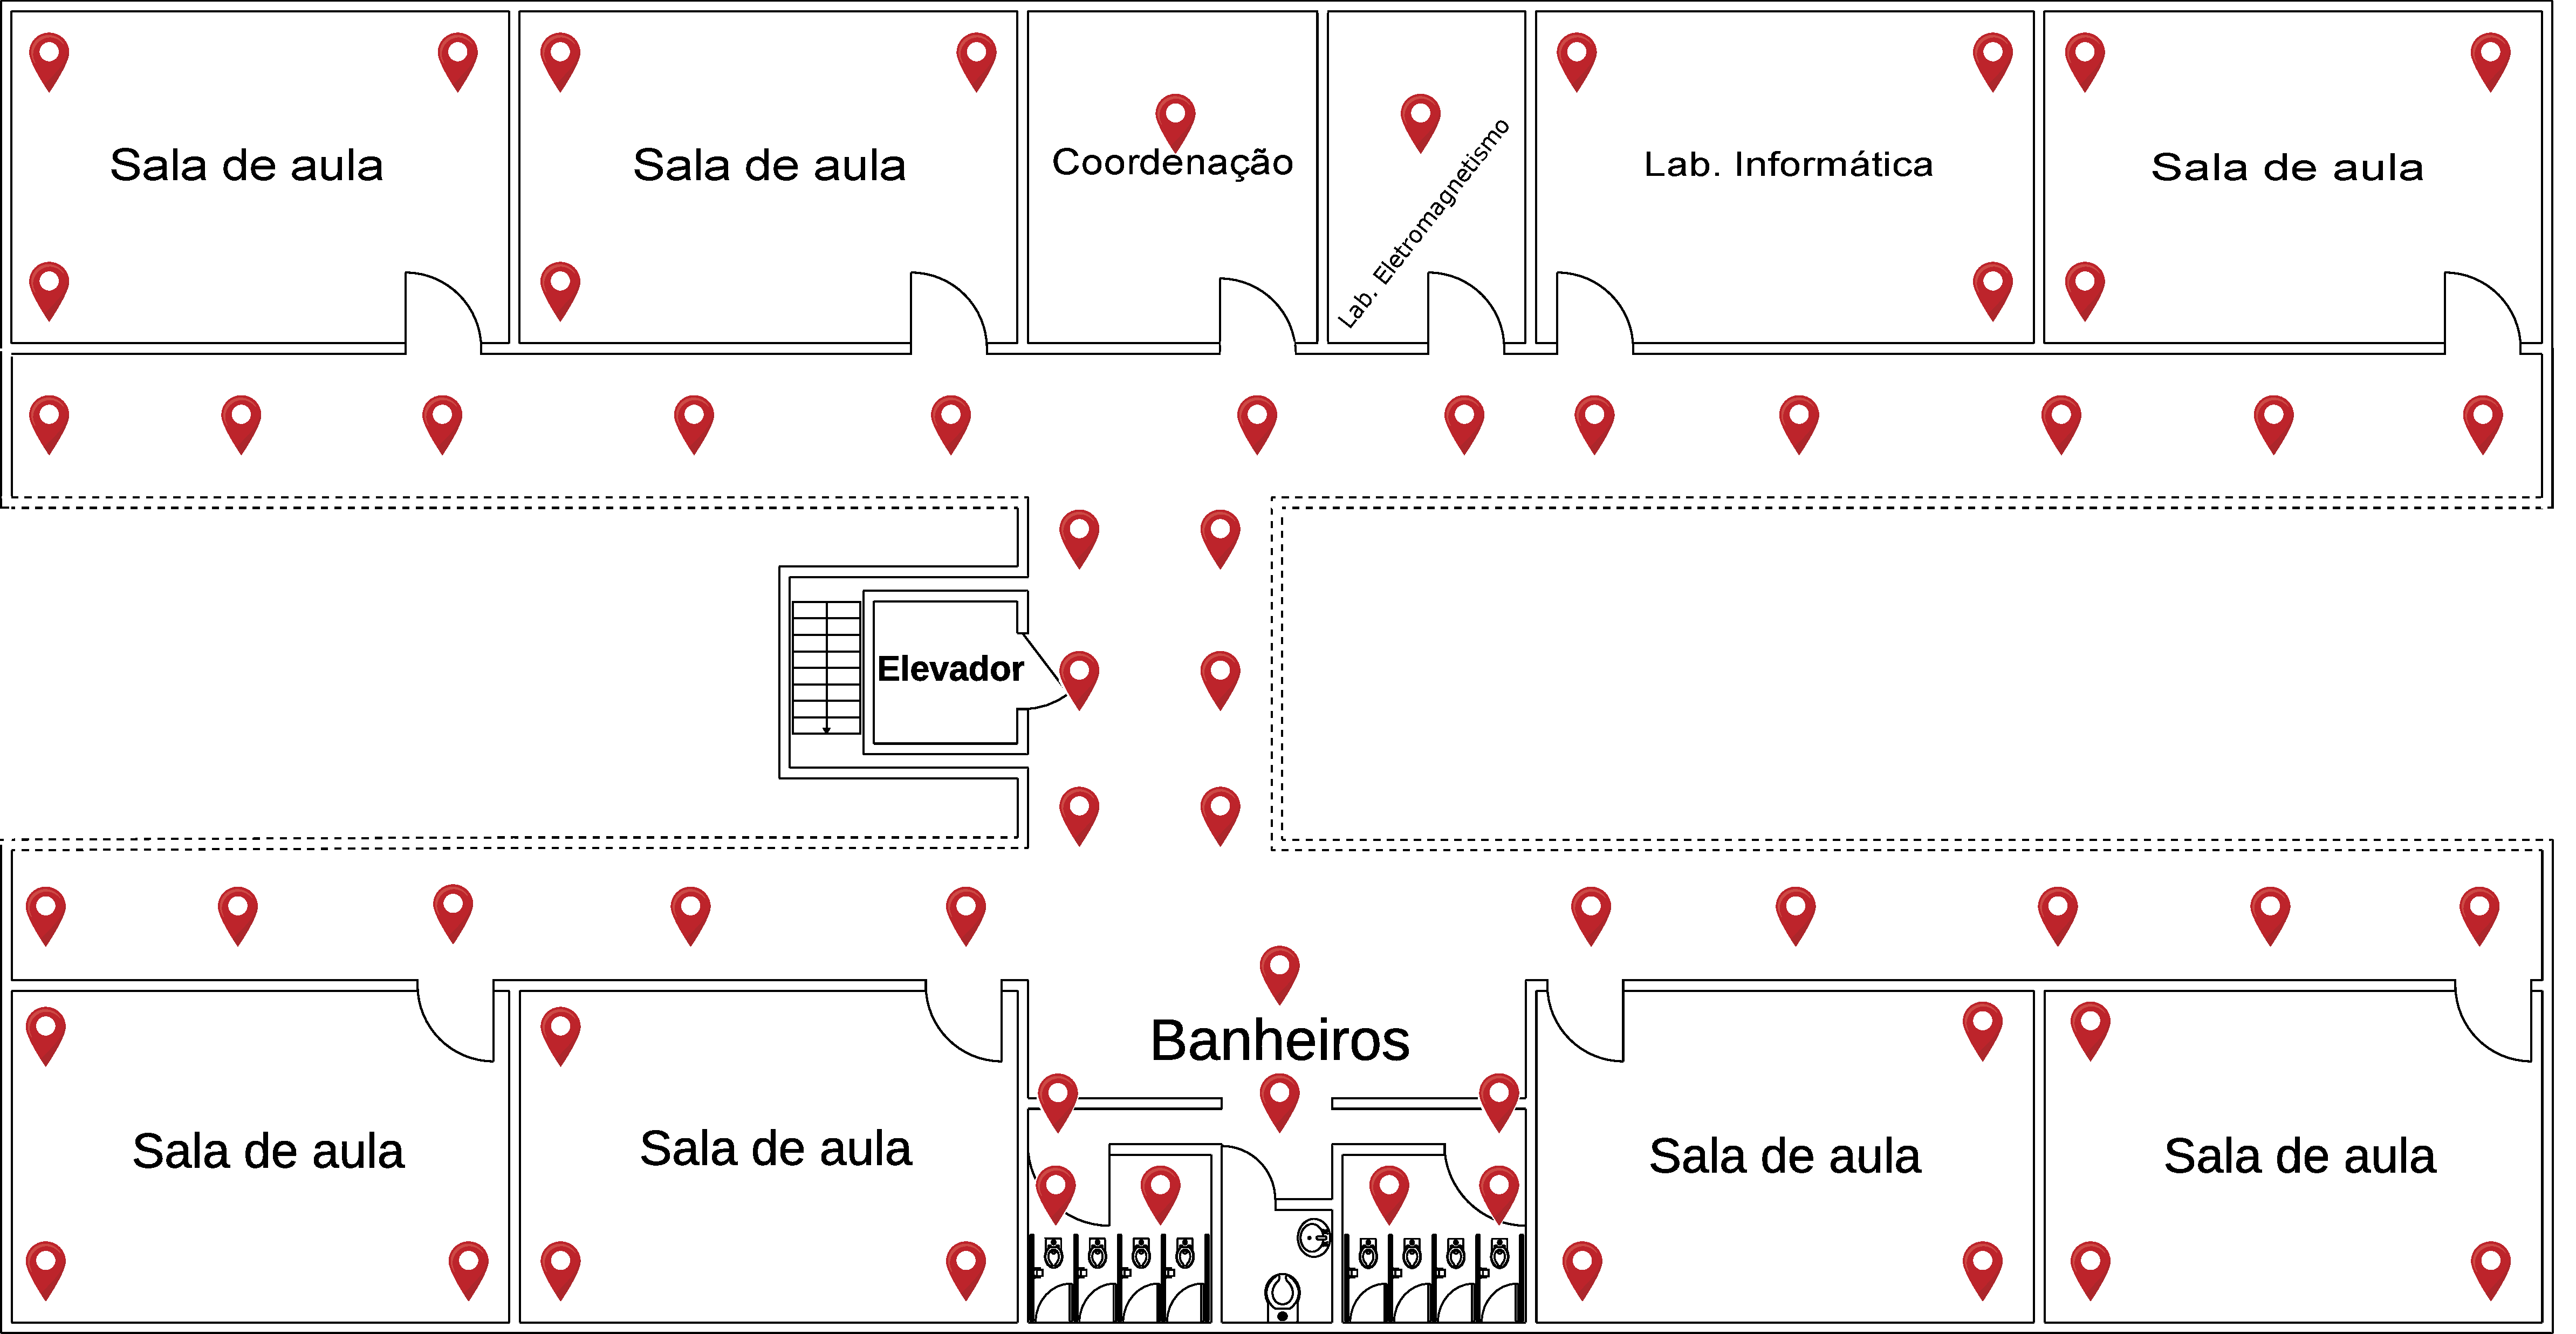
\includegraphics[scale=.2]{figuras/Pontos_Medidos_Andar02.pdf}
	}{
		\Fonte{Autor.}%
	}	
\end{figure}

\begin{figure}[H]
	\centering
	\Caption{\label{fig:pontos-andar1}Pontos medidos no térreo do Bloco Didático.}	
	\UECEfig{}{
		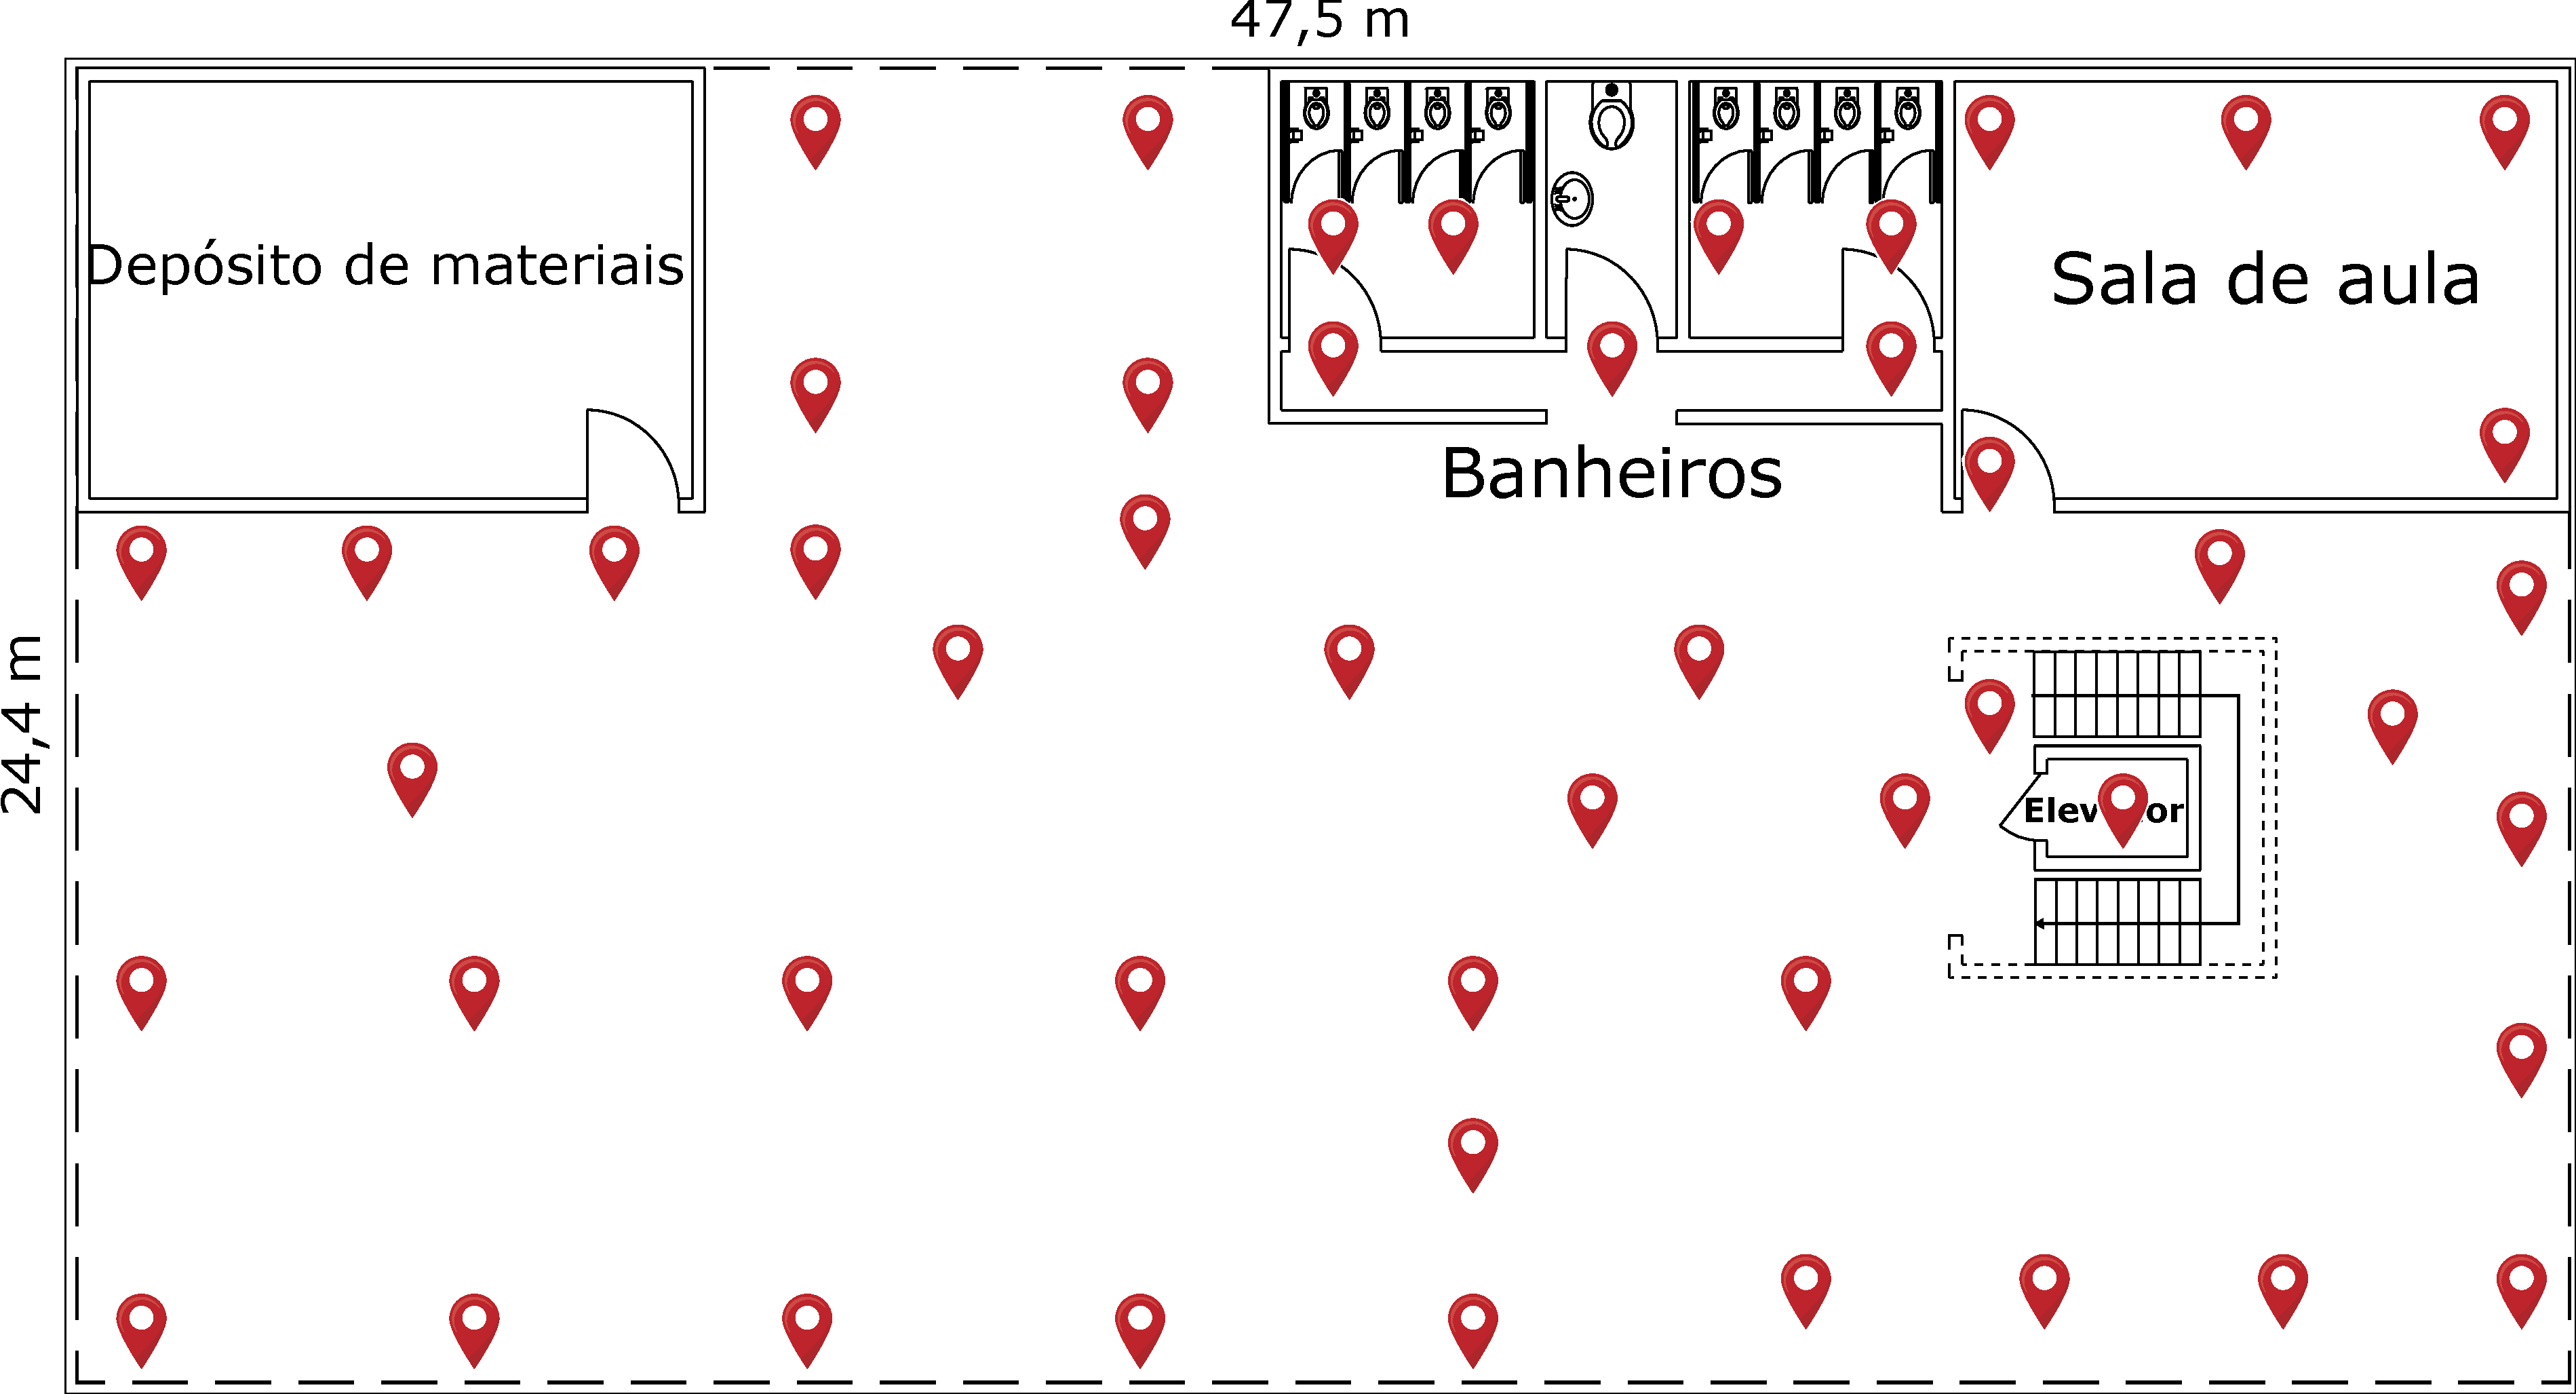
\includegraphics[scale=.255]{figuras/Pontos_Medidos_Terreo.pdf}
	}{
		\Fonte{Autor.}%
	}	
\end{figure}

\subsection{Tratamento dos dados}
\label{subsec:tratamento-dos-dados}

Após a coleta dos dados das redes sem fio detectadas no Bloco Didático, iniciou-se a etapa de tratamento dos mesmos, no qual foram analisados e depois utilizados filtros para definir quais dados das redes capturadas seriam aproveitados. \textcolor{blue}{Com o auxílio do Xirrus Wi-Fi Inspector, foram selecionadas informações que indicassem a frequência de operação e o canal utilizado pelos pontos de acesso com o objetivo de identificar interferências entre redes dentro da mesma área de cobertura.}

A \autoref{fig:networks-didatico} mostra a lista criada no Xirrus Wi-Fi Inspector com as características dos pontos de acessos detectados na varredura no térreo do Bloco Didático. A princípio, ao ser gerada a lista, são exibidos vários parâmetros pertinentes das redes Wi-Fi, tanto os que seriam úteis para o presente trabalho quanto outros não utilizados.

\begin{figure}[H]
	\centering
	\Caption{\label{fig:networks-didatico}Redes Wi-Fi detectadas pelo Xirrus Wi-Fi Inspector.}	
	\UECEfig{}{
		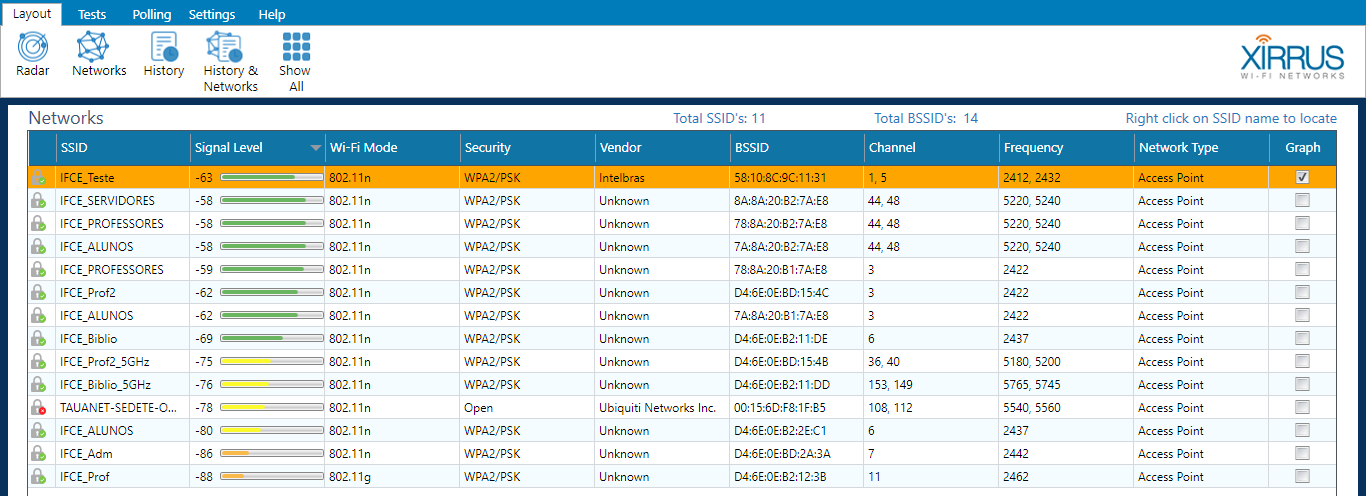
\includegraphics[scale=.43]{figuras/networks_didatic_recorte.png}
	}{
		\Fonte{Autor.}%
	}	
\end{figure}

\subsection{Geração dos mapas de calor}
\label{subsec:mapas-de-calor}

Ao final da etapa de tratamento de dados, a última fase do processo de \textit{site survey} é a geração dos mapas de calor da rede estudada.

Um mapa de calor é uma representação gráfica de dados em que os valores são representados como cores com significados determinados. Em redes sem fio, podem ser utilizados para gerar um mapa da cobertura da intensidade do sinal em toda a área de interesse, o que favorece uma análise mais visual e simplificada do ambiente \textit{wireless}. Nesse sentido, são amplamente recomendados para a demonstração dos resultados obtidos em um \textit{site survey}.

Os mapas de calor no Ekahau HeatMapper são gerados a partir da coloração entre várias cores como verde, amarelo, laranja e vermelho, que são utilizadas para representar as intensidades da potência recebida em um determinado ponto.

A \autoref{fig:escala-sinal} demonstra a barra de potência do Ekahau HeatMapper que pode receber uma variação de cores desde o verde ao vermelho.

\begin{compactitem}
	\item \textbf{Verde:} significa que o sinal recebido é muito forte.
	\item \textbf{Amarelo:} significa que a potência recebida é razoável.
	\item \textbf{Laranja:} significa que a potência obtida é ruim.
	\item \textbf{Vermelho:} significa que a potência do sinal recebido é muito fraco.
\end{compactitem}

\begin{figure}[H]
	\centering
	\Caption{\label{fig:escala-sinal}Escala de potência do sinal.}	
	\UECEfig{}{
		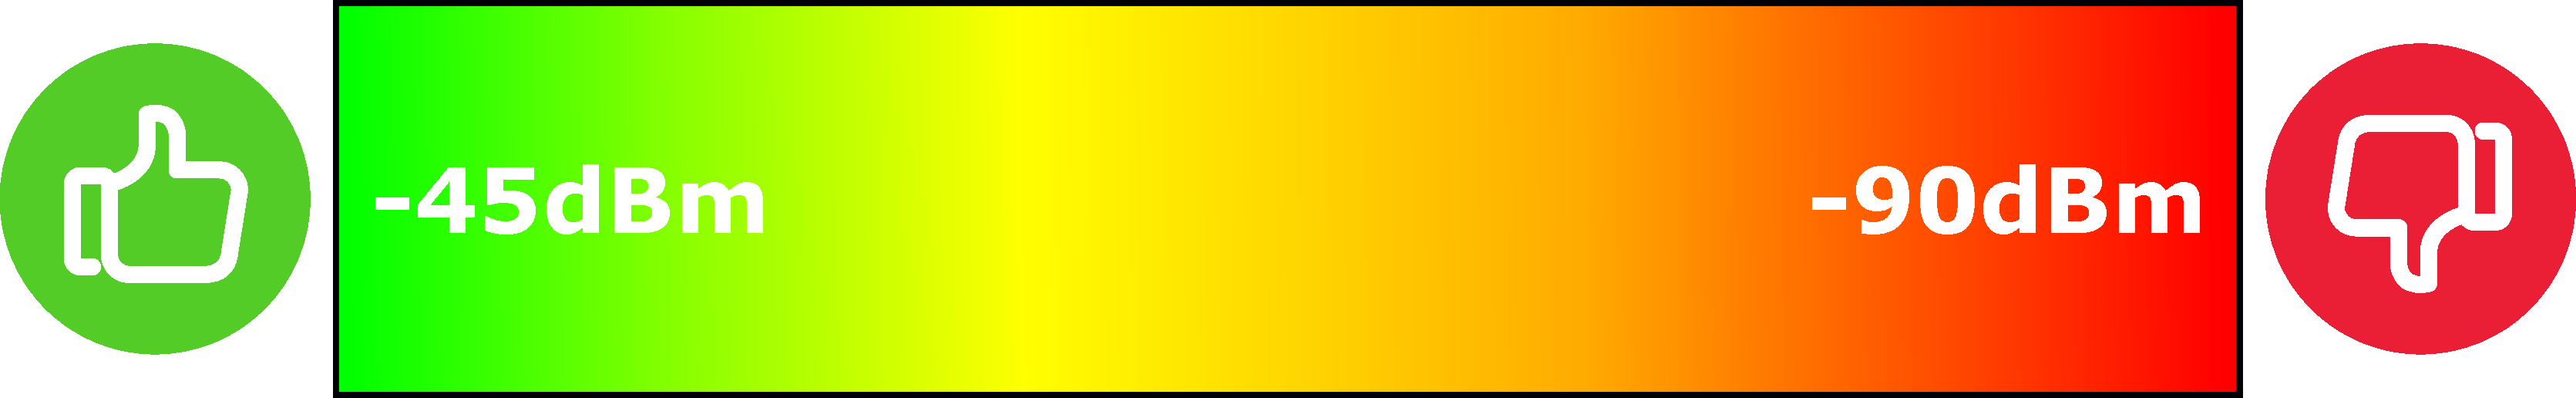
\includegraphics[scale=.185]{figuras/Escala_dBm.pdf}
	}{
		\Fonte{Autor.}%
	}	
\end{figure}

Para que os mapas fossem gerados, foram definidos valores de potência baseados em testes de distância entre um ponto de acesso e o \textit{notebook}, no qual --85dBm (ou menor) representa uma área de sombra, isto é, sem propagação suficiente de sinal, e no mapa aparecerá a tonalidade mais forte de vermelho. Isso significa que toda área do mapa que receber esse nível de sinal será considerada de perda de conectividade. Caso a potência recebida no mapa for de --45dBm (ou maior, caso o receptor seja capaz de detectá-la), isto significa que o local mapeado possui alta conectividade, sendo assim representada pela cor verde.

\section{Resultados do Site Survey}
\label{sec:resultados-site-survey}

Com a ferramenta de \textit{software} Ekahau HeatMapper foram gerados dois mapas de calor, ambas da rede Wi-Fi do Bloco Didático, o que inclui os dois pontos de acesso instalados no local. A seguir são demonstrados os resultados obtidos através da aplicação da metodologia de \textit{site survey} realizado na área já mencionada.

Devido a questões de necessidade e imprevistos, uma nova rede \textit{wireless}, com SSID IFCE\_Teste, foi implantada na sala de coordenação com as mesmas características da rede destinada aos discentes (canal e frequência de operação) para a geração dos mapas de calor. Pelo fato do ponto de acesso atribuído aos docentes (SSID IFCE\_PROFESSORES) estar localizado próximo ao dos estudantes na sala de coordenação, os mapas de calor resultantes de ambas provavelmente seriam equivalentes considerando o espaço físico do local inspecionado, apesar da frequência de operação das redes serem diferentes. Assim,  com o mapeamento de apenas uma das redes sem fio o mesmo resultado se aplicaria a outra com margem de erro desprezível para caso de verificação da propagação de radiofrequência.

A \autoref{fig:heatmapper-andar2} apresenta visualmente o mapa de calor da rede IFCE\_Teste para o térreo do Bloco Didático, e o maior nível de potência que é recebido é representado por verde e o menor nível de potência recebido é definido pela cor vermelha. Cada pequeno ponto verde interligado a outro por um segmento de reta representa o local onde foi efetuada uma medição de sinal.

\textcolor{blue}{Por algum motivo, provavelmente devido a um erro pontual, o programa Ekahau HeatMapper não exibiu a localização de determinados pontos medidos na região que abrange as duas salas de aula e o corredor do canto superior direito na \autoref{fig:heatmapper-andar2}. No entanto, não houve prejuízos significativos ao resultado final do mapeamento do primeiro andar.}

\newpage
\begin{figure}[H]
	\centering
	\Caption{\label{fig:heatmapper-andar2}Mapa de calor da rede IFCE\_Teste para o 1º andar do Bloco Didático.}	
	\UECEfig{}{
		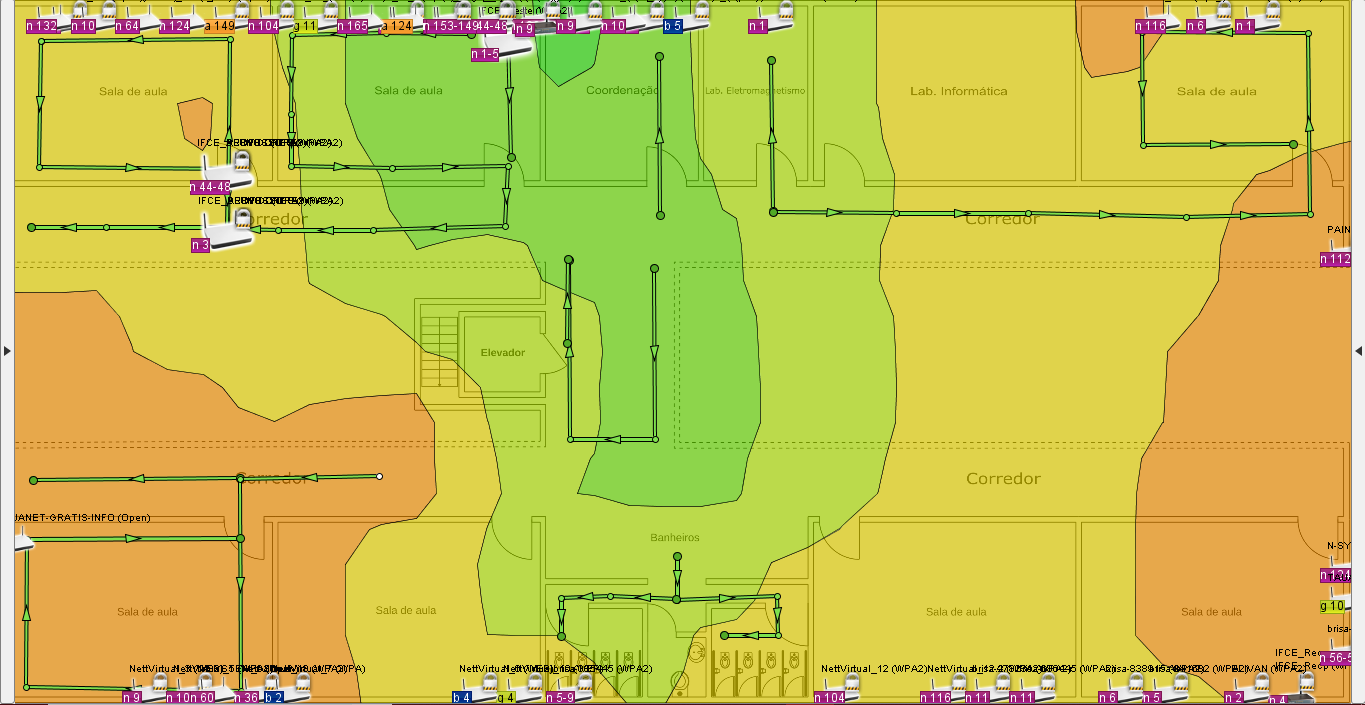
\includegraphics[scale=.65,angle=90]{figuras/heatmapper_2_andar.png}
	}{
		\Fonte{Autor.}%
	}	
\end{figure}

Como se pode observar pela área do mapa de calor da \autoref{fig:heatmapper-andar2}, as regiões que apresentaram maiores níveis de intensidade de sinal de rádio favoráveis para uma conexão foram as áreas localizadas nas imediações do centro da planta baixa, destacadas pelos tons de verde, e também pelas partições adjacentes a sala de coordenação.

Nota-se que os sinais propagados pelo térreo sofrem algumas atenuações como por exemplo nos extremos direito e esquerdo do mapa em que a coloração alaranjada simboliza locais com considerável perda de potência. Levando em consideração, pelo mapa, que as áreas mais afetadas pela perda de conectividade são as salas de aula e os corredores, frequentadas diariamente por estudantes, é indispensável a implantação de novos pontos de acesso para suprir esses locais onde o sinal perde força.

A \autoref{fig:heatmapper-andar1} representa o mapa de propagação de sinal do térreo do Bloco Didático para a rede IFCE\_Teste. A partir do mapa de calor gerado com as devidas colorações, nota-se que a rede mapeada não dispõe de uma área de cobertura que abrange todo o espaço do andar. Como é possível perceber, na maior parte do mapa as áreas apresentam tons de cor mais ``quentes'', o que significa que o ambiente não recebe bons níveis de potência de rádio para o estabelecimento de uma conexão de dados confiável. No depósito não foram realizadas medições pelo fato de o local ser usado simplesmente para armazenamento de materiais.

Logo, para que a rede IFCE\_Teste tenha uma cobertura de sinal por todo o térreo, seria necessário futuramente acrescentar mais equipamentos de acesso que irradiem sinais que alcancem as zonas com deficiência de propagação de rádio.

\begin{figure}[H]
	\centering
	\Caption{\label{fig:heatmapper-andar1}Mapa de calor da rede IFCE\_Teste para o térreo do Bloco Didático.}	
	\UECEfig{}{
		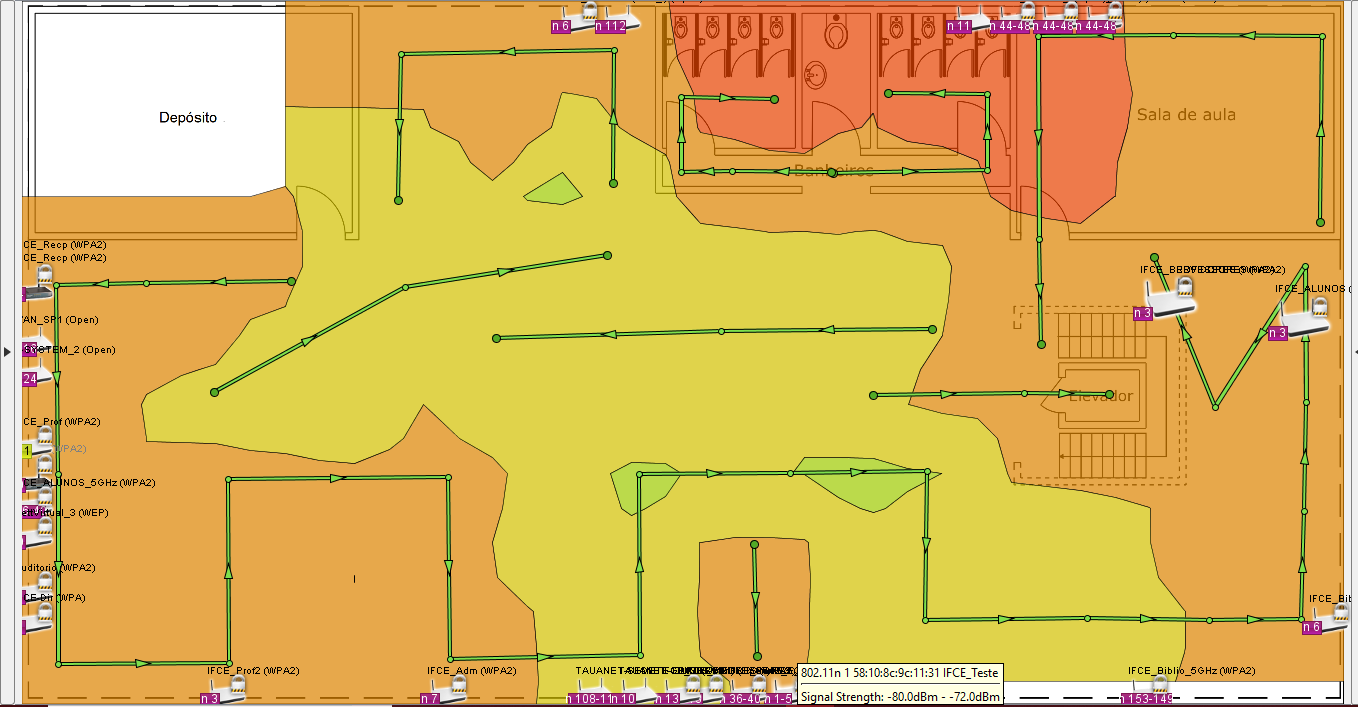
\includegraphics[scale=.64,angle=90]{figuras/heatmapper_Terreo_Editada.png}
	}{
		\Fonte{Autor.}%
	}	
\end{figure}


\section{Discussão dos Resultados}
\label{discussao-dos-resultados}

Os resultados encontrados no presente estudo evidenciam que a metodologia \textit{site survey} contribuiu significamente na avaliação da qualidade do sinal da rede Wi-Fi do Bloco Didático do IFCE Tauá, demonstrando que os dois andares mapeados apresentam níveis de propagação de radiofrequência distintos. Isso se deve ao fato de cada um dos andares possui diferentes estruturas arquitetônicas, o que influencia diretamente no alcance máximo de cada célula instalada.
	
Existem dois pontos de acesso disponíveis exclusivamente para atender o prédio, sendo um destinado aos docentes e o outro aos discentes, ambos instalados no mesmo local (sala de coordenação). Por estarem tão próximos, a cobertura de cada ponto de acesso não é adequadamente distribuída pela área, as duas zonas de serviço se sobrepõem. Porém, não há problemas de interferência entre as redes Wi-Fi, já que a rede com SSID IFCE\_Teste opera na banda de frequência de 2.4 GHz e a rede com SSID IFCE\_PROFESSORES trabalha em 5 GHz, como mostra a captura de tela da \autoref{fig:networks-didatico}. Ainda na \autoref{fig:networks-didatico} percebe-se que a rede IFCE\_PROFESSORES pode sofrer com interferências de outras redes que operam na mesma faixa de frequência e se encontram instaladas no bloco principal do \textit{campus} mas que são detectadas no Bloco Didático.

No mapa de calor gerado para o térreo do Bloco Didático (\autoref{fig:heatmapper-andar2}) observa-se a predominância de tons de verde na região central do piso. Isso quer dizer que nesse local o nível de potência recebido é forte para o estabelecimento de conexões confiáveis com a Internet. A medida que a distância de análise aumenta em relação ao ponto de acesso, as cores mudam para amarelo e laranja informando que nesses pontos a qualidade do sinal Wi-Fi diminuiu consideravelmente. Se forem consideradas as áreas livres de barreiras, como os corredores, a atenuação sofrida pelo \textit{link} de rádio é gradual, causada pela perda de espaço livre durante o percurso. 

As regiões mais extremas do mapa são as que mais perdem sinal em função da distância até o ponto de acesso, principalmente a parte superior, entretanto, no canto inferior direito o formato da zona laranja difere bastante da superior direita. Nesse local a mancha de perda concentra-se quase que unicamente na sala de aula. Analisando a imagem, observa-se que entre o ponto de acesso e a referida zona existe a presença do elevador. Por ser constituído de metal, este obstáculo absorve grande parte da energia da onda de rádio, o que prejudica sua propagação. Além disso, por ser um ambiente \textit{indoor}, é importante ponderar as perdas causadas ao sinal pela penetração da ondas de rádio em paredes: quanto mais barreiras maior a degradação. O material utilizado na construção da parede também pesa contra a propagação eletromagnética.

Em contraste ao segundo piso, o térreo do Bloco Didático possui apenas uma sala de aula, uma sala de depósito de materiais e o elevador, o restante é área aberta de convívio social dos estudantes do \textit{campus}. Por esta última descrição, seria lógico supor que o mapa de calor obtido apresentasse bons níveis de potência de sinal recebido, no entanto, o resultado final foi totalmente oposto. Como pode ser visto na mapa de calor da \autoref{fig:heatmapper-andar1}, a propagação de rádio no térreo situa-se de ruim a péssima por não existir grande concentração de tons de verde no mapa, praticamente só as cores amarelo, laranja e vermelho. Como os pontos de acesso estão confinados no térreo, as ondas de rádio obrigatoriamente atravessam o piso de concreto armado, com espessura bem maior do que as paredes das salas. Isso significa que quando o sinal passa através deste obstáculo ele já chega muito atenuado no piso inferior. No local onde fica os banheiros o sinal é ainda pior devido a existência das paredes, o que torna a conexão com a rede extremamente lenta.

\section{Propostas de Intervenção}
\label{propostas-de-intervencao}

% Sugestão de intervenção na rede sem fio
Diante de todas as discussões feitas, infere-se que intervenções na rede sem fio do Bloco Didático seriam necessárias para que a distribuição da cobertura de sinal seja mais homogênea, o que provavelmente resultaria em um nível de desempenho satisfatório para os clientes.

Tomando como base o mapa de calor do térreo (\autoref{fig:heatmapper-andar2}), a principal recomendação seria acrescentar, no mínimo, outro ponto de acesso e deslocar para fora o que está na sala de coordenação, reposicionado-os próximos aos extremos do prédio. Aconselha-se configurar os pontos de acesso para que operem em 2.4 GHz, já que ondas de rádio nessa frequência podem passar através de paredes, pisos e tetos. Portanto, elas podem chegar em locais desejáveis. Assim, áreas antes sem cobertura de sinal poderão ter maiores chances de receberem níveis mais elevados de potência em relação a rede existente. Para evitar interferência destrutiva, os equipamentos devem ser configurados em canais diferentes, de preferência 1, 6 ou 11. O possível novo posicionamento dos pontos de acesso para a abordagem sugerida pode ser visto na \autoref{fig:proposta1}.

\begin{figure}[H]
	\centering
	\Caption{\label{fig:proposta1}Proposta de posicionamento dos pontos de acesso para o 1º andar do Bloco Didático.}	
	\UECEfig{}{
		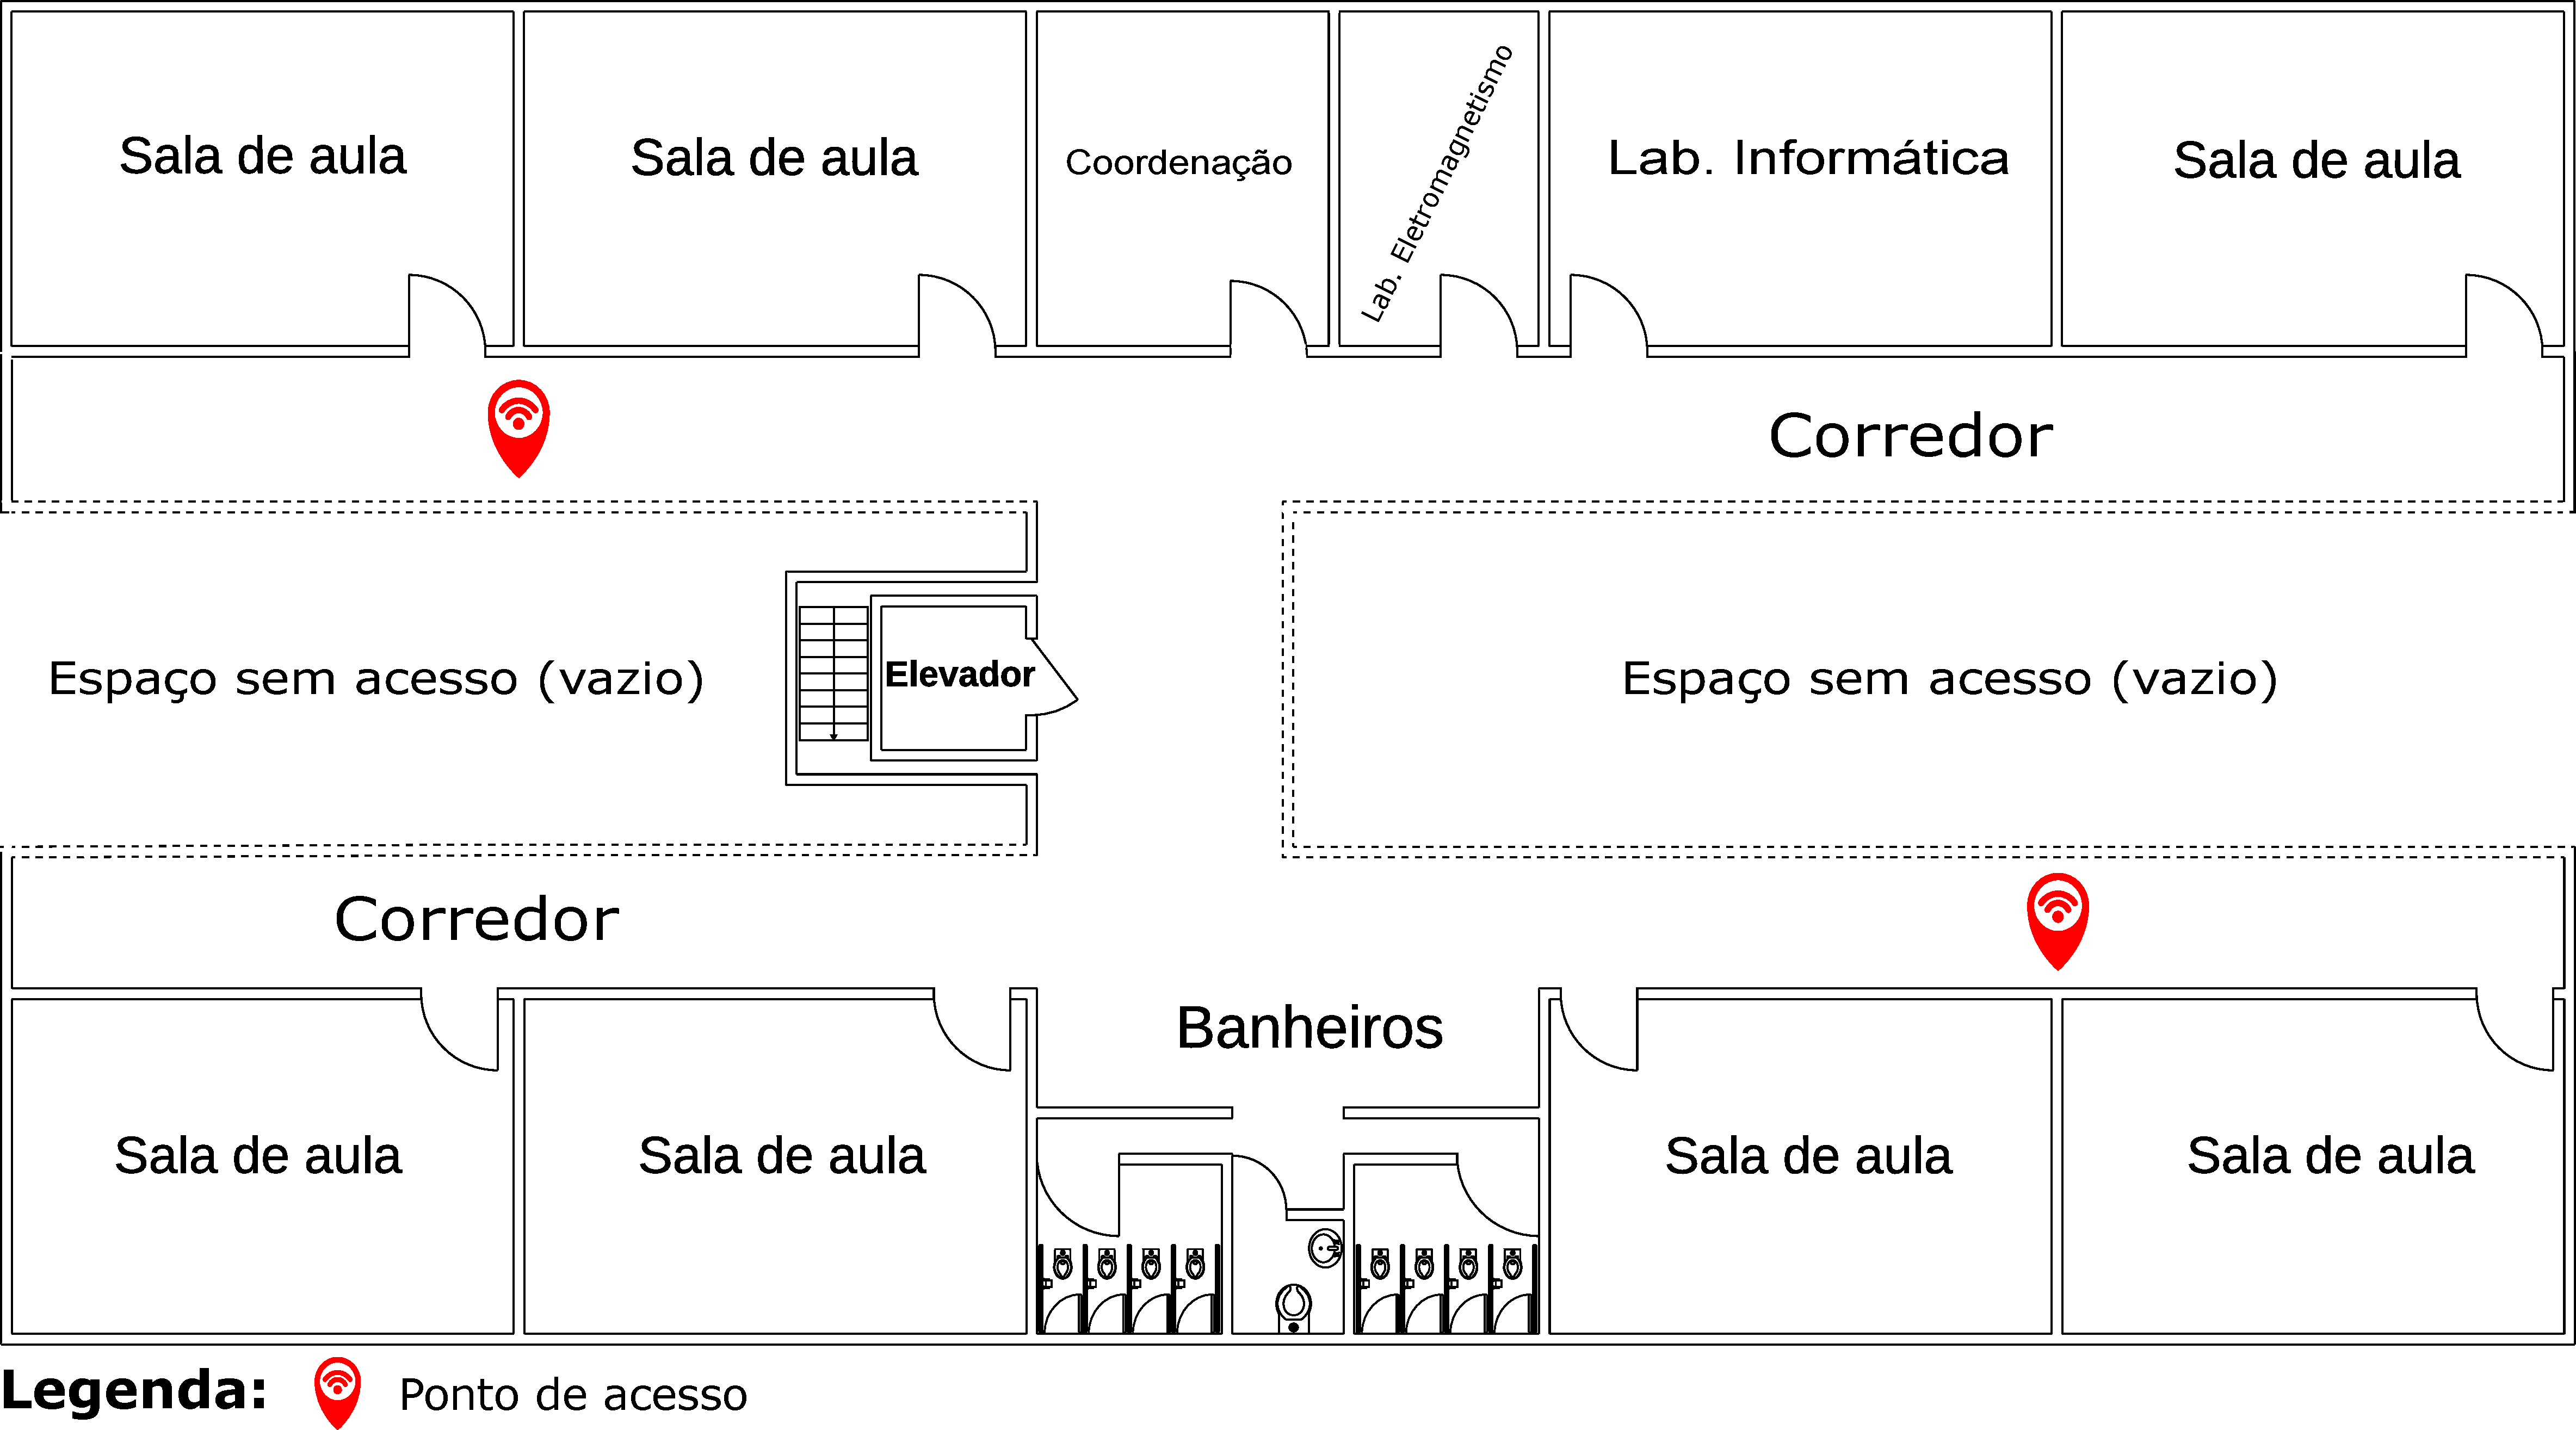
\includegraphics[scale=.18]{figuras/APs_Bloco_Andar_2_Proposta_Intervencao.pdf}
	}{
		\Fonte{Autor.}%
	}	
\end{figure}

Por não conter nenhum ponto de acesso, o térreo precisaria também de, no mínimo, dois equipamentos para prover condições satisfatórias de conexão de dados, como ilustra visualmente a  \autoref{fig:proposta2}. Ainda poderia ser utilizados pontos de acesso na frequência de 5 GHz, pois assim evitaria-se interferências com a rede do térreo, além de oferecer alta taxa de transmissão de dados em comparação com a ofertada pela banda de 2.4 GHz.

\begin{figure}[H]
	\centering
	\Caption{\label{fig:proposta2}Proposta de posicionamento dos pontos de acesso para o térreo andar do Bloco Didático.}	
	\UECEfig{}{
		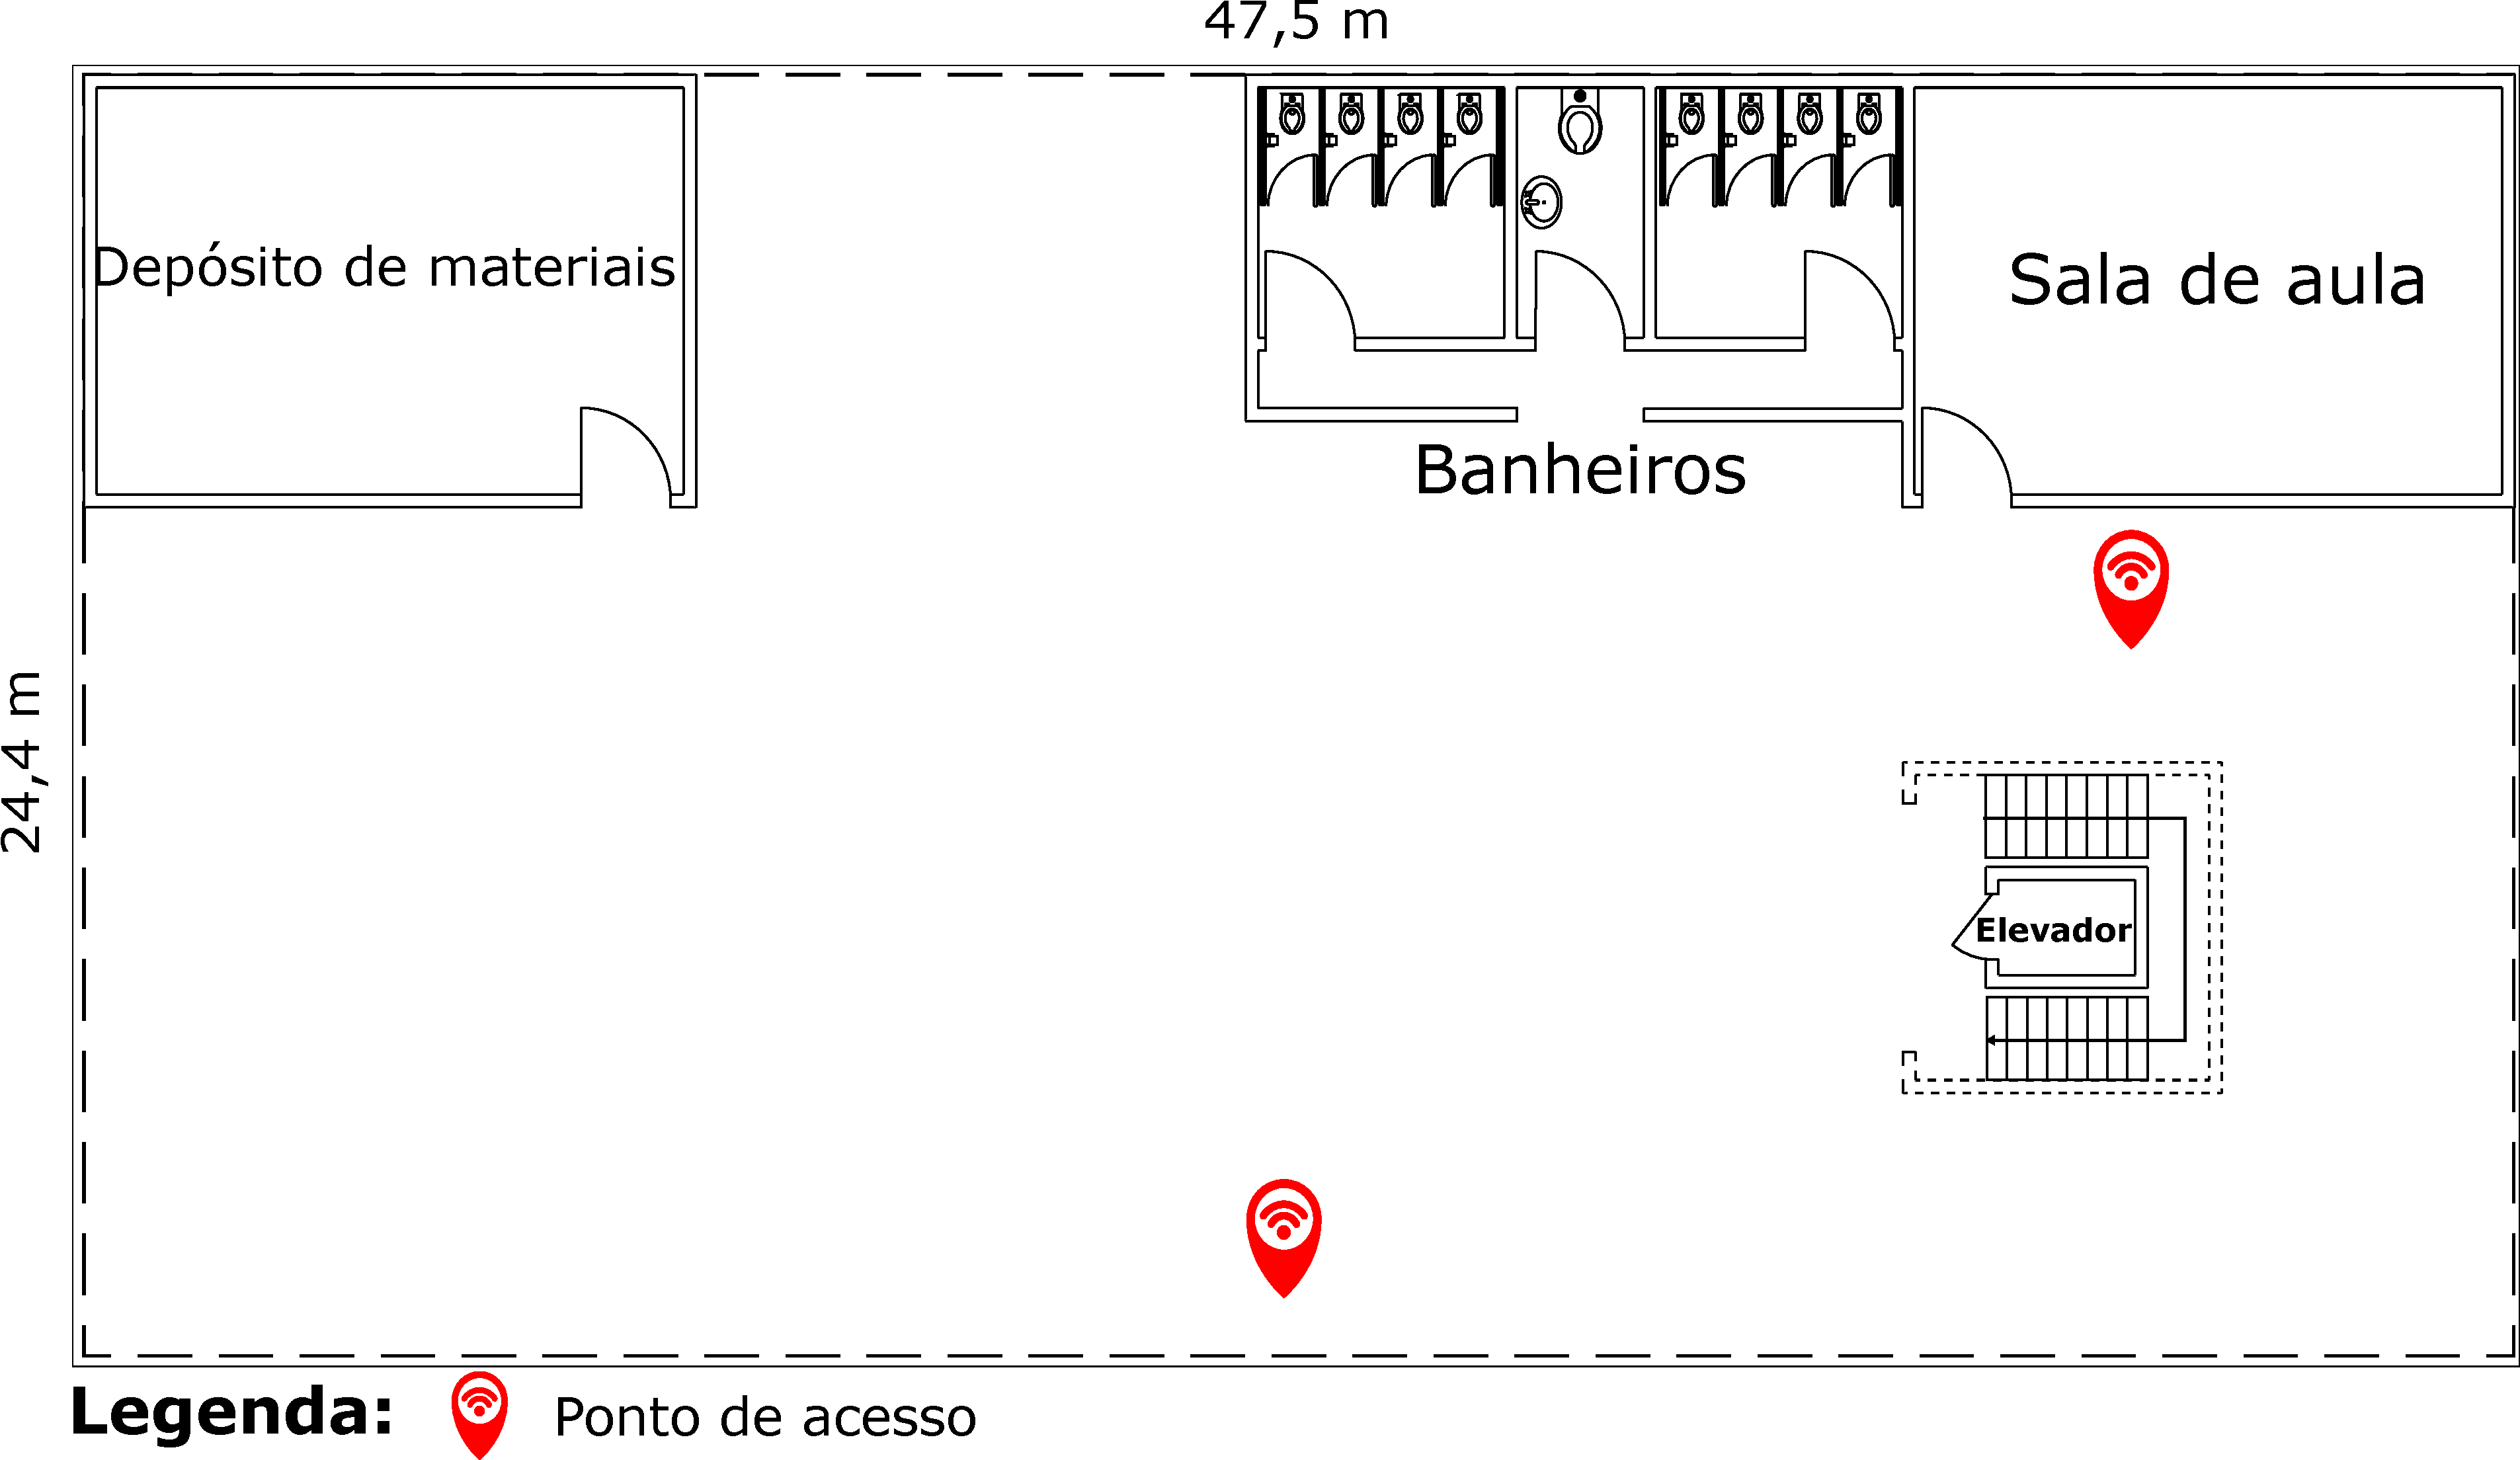
\includegraphics[scale=.22]{figuras/prop-inter-terreo.pdf}
	}{
		\Fonte{Autor.}%
	}	
\end{figure}

A justificativa para as duas propostas descritas acima fundamenta-se na utilização de pontos de acesso com antenas omnidirecionais, ou seja, que irradiam radiofrequência em todas as direções a partir do ponto de origem, distribuindo o sinal por uma área maior, ao mesmo tempo que eleva o nível de potência recebido em pontos antes castigados com a baixa conectividade. Outro motivo é que cada andar possui condições estruturais diferentes um do outro. Isso contribui diretamente no posicionamento dos pontos de acesso a fim de proporcionar as melhores condições de propagação do sinal pelo prédio.
	\chapter{Considerações Finais e Trabalhos Futuros}
\label{cap:conclusoes-e-trabalhos-futuros}

A popularidade massiva das redes sem fio tem feito com que o custo dos equipamentos caia contínua e rapidamente, enquanto a tecnologia empregada nos mesmos aumenta de forma acelerada. A propriedade do usuário ser móvel impulsionou a disseminação dos dispositivos móveis, possibilitando-os de se conectarem à Internet em qualquer local com cobertura disponível. Assim, permitir às pessoas o acesso fácil e barato à informação através da Internet é, acima de tudo, beneficiá-las diretamente com a democratização do conhecimento.

O desenvolvimento do presente estudo possibilitou a aplicação da metodologia \textit{site survey}, a qual pode contribuir para o aumento de desempenho da rede Wi-Fi do Bloco Didático do IFCE \textit{campus} Tauá. Além disso, também permitiu uma pesquisa de campo para obter dados mais consistentes sobre como ocorre a propagação de radiofrequência por todo o local de interesse.
A partir da pesquisa feita, a escolha do \textit{site survey} para a proposta do trabalho se deu graças ao seu alto grau de flexibilidade de execução tanto em redes cabeadas como em redes \textit{wireless}, voltada para a identificação de problemas. Observou-se que esta técnica pode ser empregada na avaliação de redes já em funcionamento e também no planejamento de um novo sistema, seja para pequenos projetos ou mesmo para projetos de maiores proporções.

O principal objetivo do trabalho foi alcançado, que foi utilizar as técnicas de \textit{site survey} na rede sem fio existente no Bloco Didático, pelo qual após a conclusão das etapas na rede \textit{wireless} IFCE\_Teste foi possível explorar as informações coletadas sobre o desempenho da rede Wi-Fi por toda a área. Com as informações processadas, gerou-se os mapas de calor que possibilitaram com que se identificasse as regiões com maior e menor qualidade de sinal recebido.

De acordo com os mapas de calor obtidos, constatou-se que, dos dois andares mapeados, o primeiro apresenta uma propagação de sinal pobre em relação ao segundo, onde a intensidade de potência é mais satisfatória, principalmente na área central e nas salas imediatamente próximas a coordenação.
Em relação a ferramenta de \textit{software} utilizada, o Ekahau HeatMapper teve um funcionamento livre de falhas graves, mesmo quando deixou de mostrar alguns pontos no mapa de calor do térreo do Bloco Didático. Mesmo sendo um programa gratuito, atendeu aos requisitos exigidos para a execução das atividades do \textit{site survey}.

Todos os resultados apresentados e discutidos neste trabalho, adquiridas por meio de um \textit{site survey}, demonstram que, devido a natureza complexa e aleatória da propagação de ondas de rádio, é importante definir métodos para avaliação/planejamento de redes sem fio que proporcionem resultados confiáveis com os quais possam ser utilizados para que se tenha uma melhor performance em redes do tipo Wi-Fi.

\section{Trabalhos Futuros}
\label{sec:trabalhos-futuros}

Como proposta de trabalhos posteriores, a metodologia \textit{site survey} pode ser implementada buscando novas linhas de pesquisa e estudo em projetos que envolvam redes sem fio, tais como:

\begin{compactitem}
	\item Realizar um novo \textit{site survey} no Bloco Didático para que mais parâmetros possam ser analisados, como tráfego de dados, interferências e a opinião dos usuários a respeito de aspectos da rede.
	
	%\item \textcolor{blue}{Aplicar o \textit{site survey} para a avaliação da nova rede sem fio implantada no Bloco Didático e comparar os resultados com os obtidos por este trabalho.}
	
	\item Expandir a aplicação do \textit{site survey} para todo o IFCE \textit{campus} Tauá, o que inclui o estacionamento (ambiente \textit{outdoor}) e o bloco principal (ambiente \textit{indoor}) para uma investigação mais completa.
\end{compactitem}



		
	% Elementos pós-textuais
	
	% Caso utilze o TeXstudio, a bibliográfia será inserida automaticamente :).
	\bibliography{elementos-pos-textuais/referencias}
	
	
%	\imprimirglossario	
%	\imprimirapendices
%		% Adicione aqui os apendices do seu trabalho
%		\apendice{Lorem Ipsum}
\label{ap:lorem-ipsum}

\lipsum[1]
%		\apendice{Modelo de Capa}
\label{ap:modelo-de-capa}

\lipsum[1]

%		\apendice{Termo de Fiel Depositário}
\label{ap:termo-de-fiel-depositario}

\noindent \textbf{Pesquisa:} ANÁLISE DA MORTALIDADE INFANTIL COM MALFORMAÇÕES CONGÊNITAS.

\noindent Pelo presente instrumento que atende às exigências legais, a Sra. Maria Consuelo Martins Saraiva, ``fiel depositário'' com o cargo de Secretária Municipal de Saúde de Iracema, após ter tomado conhecimento do protocolo de pesquisa intitulado: ANÁLISE DA MORTALIDADE INFANTIL COM MALFORMAÇÕES CONGÊNITAS. Analisando a repercussão desse estudo no contexto da saúde pública e epidemiologia, autoriza Karla Maria da Silva Lima, enfermeira, aluna do Curso de Mestrado Acadêmico em Enfermagem da Universidade Estadual do Ceará (UECE), sob orientação do Prof. Dr. José Maria de Castro, da UECE, ter acesso aos bancos de dados do Sistema de Informação sobre Nascidos Vivos e do Sistema de Informação sobre Mortalidade da Secretaria Municipal de Saúde de Iracema, objeto deste estudo, e que se encontram sob sua total responsabilidade. Fica claro que o Fiel Depositário pode a qualquer momento retirar sua AUTORIZAÇÃO e ciente de que todas as informações prestadas tornar-se-ão confidenciais e guardadas por força de sigilo profissional, assegurando que os dados obtidos da pesquisa serão somente utilizados para estudo.	
%	\imprimiranexos
%		% Adicione aqui os anexos do seu trabalho
%		\anexo{Exemplo de Anexo}
\label{an:exemplo-de-anexo}

\lipsum[13]		
%		\anexo{Dinâmica das classes sociais}
\label{an:dinamica-das-classes-sociais}

\lipsum[14]
\index{AAA}
%	\imprimirindice
\end{document}